% Options for packages loaded elsewhere
\PassOptionsToPackage{unicode}{hyperref}
\PassOptionsToPackage{hyphens}{url}
%
\documentclass[
]{article}
\usepackage{amsmath,amssymb}
\usepackage{lmodern}
\usepackage{setspace}
\usepackage{iftex}
\ifPDFTeX
  \usepackage[T1]{fontenc}
  \usepackage[utf8]{inputenc}
  \usepackage{textcomp} % provide euro and other symbols
\else % if luatex or xetex
  \usepackage{unicode-math}
  \defaultfontfeatures{Scale=MatchLowercase}
  \defaultfontfeatures[\rmfamily]{Ligatures=TeX,Scale=1}
\fi
% Use upquote if available, for straight quotes in verbatim environments
\IfFileExists{upquote.sty}{\usepackage{upquote}}{}
\IfFileExists{microtype.sty}{% use microtype if available
  \usepackage[]{microtype}
  \UseMicrotypeSet[protrusion]{basicmath} % disable protrusion for tt fonts
}{}
\usepackage{xcolor}
\IfFileExists{xurl.sty}{\usepackage{xurl}}{} % add URL line breaks if available
\IfFileExists{bookmark.sty}{\usepackage{bookmark}}{\usepackage{hyperref}}
\hypersetup{
  pdftitle={Manuscript: Detecting differences in Size Spectra},
  pdfauthor={Justin Pomeranz1,; James R. Junker2,3; Vojsava Gjoni4; Jeff S. Wesner4},
  hidelinks,
  pdfcreator={LaTeX via pandoc}}
\urlstyle{same} % disable monospaced font for URLs
\usepackage[margin=1in]{geometry}
\usepackage{color}
\usepackage{fancyvrb}
\newcommand{\VerbBar}{|}
\newcommand{\VERB}{\Verb[commandchars=\\\{\}]}
\DefineVerbatimEnvironment{Highlighting}{Verbatim}{commandchars=\\\{\}}
% Add ',fontsize=\small' for more characters per line
\usepackage{framed}
\definecolor{shadecolor}{RGB}{248,248,248}
\newenvironment{Shaded}{\begin{snugshade}}{\end{snugshade}}
\newcommand{\AlertTok}[1]{\textcolor[rgb]{0.94,0.16,0.16}{#1}}
\newcommand{\AnnotationTok}[1]{\textcolor[rgb]{0.56,0.35,0.01}{\textbf{\textit{#1}}}}
\newcommand{\AttributeTok}[1]{\textcolor[rgb]{0.77,0.63,0.00}{#1}}
\newcommand{\BaseNTok}[1]{\textcolor[rgb]{0.00,0.00,0.81}{#1}}
\newcommand{\BuiltInTok}[1]{#1}
\newcommand{\CharTok}[1]{\textcolor[rgb]{0.31,0.60,0.02}{#1}}
\newcommand{\CommentTok}[1]{\textcolor[rgb]{0.56,0.35,0.01}{\textit{#1}}}
\newcommand{\CommentVarTok}[1]{\textcolor[rgb]{0.56,0.35,0.01}{\textbf{\textit{#1}}}}
\newcommand{\ConstantTok}[1]{\textcolor[rgb]{0.00,0.00,0.00}{#1}}
\newcommand{\ControlFlowTok}[1]{\textcolor[rgb]{0.13,0.29,0.53}{\textbf{#1}}}
\newcommand{\DataTypeTok}[1]{\textcolor[rgb]{0.13,0.29,0.53}{#1}}
\newcommand{\DecValTok}[1]{\textcolor[rgb]{0.00,0.00,0.81}{#1}}
\newcommand{\DocumentationTok}[1]{\textcolor[rgb]{0.56,0.35,0.01}{\textbf{\textit{#1}}}}
\newcommand{\ErrorTok}[1]{\textcolor[rgb]{0.64,0.00,0.00}{\textbf{#1}}}
\newcommand{\ExtensionTok}[1]{#1}
\newcommand{\FloatTok}[1]{\textcolor[rgb]{0.00,0.00,0.81}{#1}}
\newcommand{\FunctionTok}[1]{\textcolor[rgb]{0.00,0.00,0.00}{#1}}
\newcommand{\ImportTok}[1]{#1}
\newcommand{\InformationTok}[1]{\textcolor[rgb]{0.56,0.35,0.01}{\textbf{\textit{#1}}}}
\newcommand{\KeywordTok}[1]{\textcolor[rgb]{0.13,0.29,0.53}{\textbf{#1}}}
\newcommand{\NormalTok}[1]{#1}
\newcommand{\OperatorTok}[1]{\textcolor[rgb]{0.81,0.36,0.00}{\textbf{#1}}}
\newcommand{\OtherTok}[1]{\textcolor[rgb]{0.56,0.35,0.01}{#1}}
\newcommand{\PreprocessorTok}[1]{\textcolor[rgb]{0.56,0.35,0.01}{\textit{#1}}}
\newcommand{\RegionMarkerTok}[1]{#1}
\newcommand{\SpecialCharTok}[1]{\textcolor[rgb]{0.00,0.00,0.00}{#1}}
\newcommand{\SpecialStringTok}[1]{\textcolor[rgb]{0.31,0.60,0.02}{#1}}
\newcommand{\StringTok}[1]{\textcolor[rgb]{0.31,0.60,0.02}{#1}}
\newcommand{\VariableTok}[1]{\textcolor[rgb]{0.00,0.00,0.00}{#1}}
\newcommand{\VerbatimStringTok}[1]{\textcolor[rgb]{0.31,0.60,0.02}{#1}}
\newcommand{\WarningTok}[1]{\textcolor[rgb]{0.56,0.35,0.01}{\textbf{\textit{#1}}}}
\usepackage{graphicx}
\makeatletter
\def\maxwidth{\ifdim\Gin@nat@width>\linewidth\linewidth\else\Gin@nat@width\fi}
\def\maxheight{\ifdim\Gin@nat@height>\textheight\textheight\else\Gin@nat@height\fi}
\makeatother
% Scale images if necessary, so that they will not overflow the page
% margins by default, and it is still possible to overwrite the defaults
% using explicit options in \includegraphics[width, height, ...]{}
\setkeys{Gin}{width=\maxwidth,height=\maxheight,keepaspectratio}
% Set default figure placement to htbp
\makeatletter
\def\fps@figure{htbp}
\makeatother
\setlength{\emergencystretch}{3em} % prevent overfull lines
\providecommand{\tightlist}{%
  \setlength{\itemsep}{0pt}\setlength{\parskip}{0pt}}
\setcounter{secnumdepth}{-\maxdimen} % remove section numbering
\newlength{\cslhangindent}
\setlength{\cslhangindent}{1.5em}
\newlength{\csllabelwidth}
\setlength{\csllabelwidth}{3em}
\newlength{\cslentryspacingunit} % times entry-spacing
\setlength{\cslentryspacingunit}{\parskip}
\newenvironment{CSLReferences}[2] % #1 hanging-ident, #2 entry spacing
 {% don't indent paragraphs
  \setlength{\parindent}{0pt}
  % turn on hanging indent if param 1 is 1
  \ifodd #1
  \let\oldpar\par
  \def\par{\hangindent=\cslhangindent\oldpar}
  \fi
  % set entry spacing
  \setlength{\parskip}{#2\cslentryspacingunit}
 }%
 {}
\usepackage{calc}
\newcommand{\CSLBlock}[1]{#1\hfill\break}
\newcommand{\CSLLeftMargin}[1]{\parbox[t]{\csllabelwidth}{#1}}
\newcommand{\CSLRightInline}[1]{\parbox[t]{\linewidth - \csllabelwidth}{#1}\break}
\newcommand{\CSLIndent}[1]{\hspace{\cslhangindent}#1}
\usepackage{lineno}
\usepackage{amsmath}
\usepackage{indentfirst}
\linenumbers
\newcommand{\beginsupplement}{ \setcounter{table}{0} \renewcommand{\thetable}{S\arabic{table}} \setcounter{figure}{0} \renewcommand{\thefigure}{S\arabic{figure}}}
\ifLuaTeX
  \usepackage{selnolig}  % disable illegal ligatures
\fi

\title{Manuscript: Detecting differences in Size Spectra}
\author{Justin Pomeranz\textsuperscript{1,*} \and James R.
Junker\textsuperscript{2,3} \and Vojsava
Gjoni\textsuperscript{4} \and Jeff S. Wesner\textsuperscript{4}}
\date{24 September, 2022}

\begin{document}
\maketitle

{
\setcounter{tocdepth}{2}
\tableofcontents
}
\setstretch{1}
\textsuperscript{1} Colorado Mesa University, Grand Junction, CO, USA\\
\textsuperscript{2} Great Lakes Research Center, Michigan Technological
University, Houghton, MI USA\\
\textsuperscript{3} Louisiana Universities Marine Consortium, Chauvin,
LA USA\\
\textsuperscript{4} Dept. of Biology, University of South Dakota,
Vermillion, SD, USA

\textsuperscript{*} Correspondence:
\href{mailto:jfpomeranz@gmail.com}{Justin Pomeranz
\textless{}\href{mailto:jfpomeranz@gmail.com}{\nolinkurl{jfpomeranz@gmail.com}}\textgreater{}}

\textbf{NOTE} I'm still working on integrating with Zotero and importing
all the necessary references (thanks Jim for the help and
instructions!). Don't worry about the \textbf{??} references in the
rendered version for now.

\textbf{Savina} I'm particularly keen to get your feedback on this. I
think you mentioned including some other references and discussion in
Jeff's Bayesian model paper. If you think they fit in here please let me
know or feel free to include them. Likewise, please include any other
comments you have, or if you have any insight into how the
interpretation of results from different methods would vary.

\hypertarget{abstract}{%
\section{Abstract}\label{abstract}}

\begin{enumerate}
\def\labelenumi{\arabic{enumi}.}
\tightlist
\item
  Size spectra represent a fundamental attribute of community
  organization and are increasingly being used in assessments of fresh
  waters.
\item
  Many methods have been proposed for constructing size spectra
  relationships, but recent work has shown that varied methods return
  biased estimates of relationship parameters, and different methods in
  fact are not estimating the same parameter. Despite this variability
  in estimates, it is unclear if the relative change across
  environmental gradients is consistent across methodologies. Here, we
  simulate data sets across an hypothetical environmental gradient and
  estimate the size spectra parameter (slope or exponent, depending on
  method) at each site, and, importantly, estimate the relationship of
  parameters across the hypothetical gradient. We also use two
  previously published body size datasets across an anthropogenic stress
  gradient and an environmental temperature gradient and assess how the
  conclusions of these studies would vary based on methods used.
\item
  We find that maximum likelihood methods always perform as well or
  better than common binning methods. Additionally, the variance in
  estimates using MLE methods is markedly reduced when compared to
  binning methods.
\item
  The uncertainty and variation in estimates when using binning methods
  is often greater than or equal to the variation previously published
  in experimental and observational studies, bringing into question the
  effect size of previously published results. However, re-analysis of
  two previously published datasets does not markedly alter the
  conclusions reached. Further study is needed to identify how and when
  these estimates may be biased, and when the general pattern of results
  can be considered to be ``true''.
\end{enumerate}

\hypertarget{introduction}{%
\section{Introduction}\label{introduction}}

Body size distributions are a fundamental characteristic of communities.
The remarkable consistency of these relationships across spatiotemporal
scales and habitat types has led them to be recommended as a
``universal'' indicator of ecological status (Petchey and Belgrano
2010)(Petchey and Belgrano 2010). Size metrics have commonly been used
in marine systems, and are increasingly being applied to assess the
condition of freshwater ecosystems (Martinez et al.~2016, Pomeranz
2018)(Pomeranz et al. 2019, \textbf{martinez2016?}).

Individual size distributions (ISD, also referred to as abundance size
spectra) are commonly used. Generally, there is a negative relationship
between body size (M) and abundance (N). Theoretical and empirical data
support this relationship being described as a simple power law with
exponent \(\lambda\) in the form of \(N \sim M^{\lambda}\). Commonly,
\(N\) is the count of body sizes grouped into bins, and \(\lambda\) is
estimated from OLS regressions of log transformed data of \(N\) and the
mid point of the body size bin \(M_{bin}\):
\(\log(N_{count}) = \lambda \log(M_{bin})\). Myriad binning methods have
been proposed, including linear and logarithmic bin widths. Likewise,
methods can rely on the absolute count in the bins as well as
normalization techniques where the count is divided by the bin width
(especially common with logarithmic binning). Alternatively, \(\lambda\)
can be estimated directly using maximum likelihood techniques.

Previous work has shown that the estimates of \(\lambda\) differ between
MLE and OLS techniques. OLS methods are particularly sensitive to
decisions made in the binning process. Simulation studies have shown
that MLE offers consistently more accurate estimates of \(\lambda\)
(White et al.~2007, Edwards et al.~2017)(White et al. 2007, Edwards et
al. 2017), and reanalysis of empirical datasets also indicates that the
conclusions are dependent on the methodology used (White et al.~2007,
Edwards et al.~2020)(White et al. 2007, Edwards et al. 2020). However,
recent empirical analysis of stream macroinvertebrate communities across
the NAtional Ecological Observatory Network (NEON, USA) showed that
while the estimates of \(\lambda\) varied, the relative change across
the environmental gradient was consistent regardless of method used
(Pomeranz et al.~2022)(Pomeranz et al. 2022). While there is a growing
consensus that MLE methods offer more reliable estimates of \(\lambda\),
and binning methods result in biased estimates, it remains unclear if
these biases are consistent and systematic or stochastic, and whether or
not the relative change in ISD parameters is consistent across space and
time. In other words, if the data within a study are all treated the
same, does a relative change of OLS slope parameters of 0.1 coincide
with a relative change of MLE estimates of 0.1? In order to answer this
question, we simulate body size observations from bounded power law
distributions with varied \(\lambda\) exponents across a hypothetical
environmental gradient and compare the results obtained using three
different methodologies common in the literature. In addition, we
re-analyze two previously published datasets of stream community body
sizes across a stress and environmental gradient. We find that the MLE
method more accurately estimates the site-specific \(\lambda\) exponents
as well as the relative change in exponents across the hypothetical
gradient, as well as having smaller variation. The logarthmic binning
methods generally perform well, but have larger confidence intervals
around the estimates. However, the overall conclusions of previously
published empirical data sets are not dependent on the method used.

\hypertarget{methods}{%
\section{Methods}\label{methods}}

\hypertarget{data-simulation}{%
\subsection{Data Simulation}\label{data-simulation}}

In order to investigate the performance of commonly used methods, we
simulate body size observations from a bounded power law distribution
using the inverse method, as described in Edwards et al.~(2017)(2017).
Let \(M\) be a random variable of body sizes described by the
probability density function:

\[f(M) = CM^\lambda, M_{min} \le M \le M_{max} \]

\(M_{min} = 0.0026\) and \(M_{max} = 1.2 *10^3\). These values are based
on empirical body sizes of stream benthic communities reported in
Pomeranz et al.~(2020)(Pomeranz et al. 2022). Our results are not
dependent on the range of body sizes, and we show the results of other
body size ranges in the supplemental information.

For the main analysis, presented here, we sampled \(n = 1000\) body
sizes from distributions described by five different \(\lambda\)'s:
(-1.5, -1.75, -2.00, -2.25, -2.5), such that our model for \(\lambda\)
is:

\[\lambda = Norm(\alpha -0.5X, \sigma)\]

Each value of \(\lambda\) was assumed to come from a community across a
hypothetical environmental gradient \(X\). Values of \(X\) for each
community are uniformly distributed from -1 to 1. We repeated the data
simulation 1000 times (reps). The main results presented here were not
dependent on the range of \emph{x}-values or the number of sites
(supplemental information).

\hypertarget{sample-size-n}{%
\subsubsection{\texorpdfstring{Sample size,
\(n\)}{Sample size, n}}\label{sample-size-n}}

The number of observations in our simulations may bias the results.
Therefore, we repeated the simulations described above, but varied the
sample size \(n\). We tested values of
\(n = 200, 500, 1000, 5000, 10 000\).

\hypertarget{no-relationship}{%
\subsubsection{``No'' relationship}\label{no-relationship}}

It is possible that our sampling or simulation framework could bias the
results obtained. In order to assess whether or not our simulations are
robust to this, we performed independent random samples from a bounded
power law for five communities across a hypothetical gradient as
described above, but we set \(\lambda = -2\) for all five communities.
Hence, we are simulating a scenario where the size spectra relationship
is invariant to our hypothetical environmental gradient, and we should
expect the estimated relationship coefficient \(\beta_1 = 0\).

\hypertarget{finer-resolution-of-lambda-values}{%
\subsection{\texorpdfstring{Finer resolution of \(\lambda\)
values}{Finer resolution of \textbackslash lambda values}}\label{finer-resolution-of-lambda-values}}

For the main analysis, we were interested in determining whether or not
the methods were able to detect relatively coarse changes to size
spectra parameters, specifically, a change of 0.5 units across each
value of \(X\), or an absolute change in \(\lambda\) values of 1.0
units. However, many seminal works on variation in size spectra
relationships in freshwater are on a much finer scale (on the order 0f
0.1 to 0.25 units). Therefore, we performed simulations as described
above, but varied \(\lambda\) from -1.9 to -2.1 across the hypothetical
environmental gradient. This equates to a know relationship coefficient
of \(\beta_1 = 0.1\) across the hypothetical gradient, and an absolute
change of 0.2 units.

\hypertarget{estimation-of-size-spectra-parameter-lambda}{%
\subsection{\texorpdfstring{Estimation of Size spectra parameter
\(\lambda\)}{Estimation of Size spectra parameter \textbackslash lambda}}\label{estimation-of-size-spectra-parameter-lambda}}

For each sample of \(M\) and each of the 1000 replicates, we estimated
the exponent \(\lambda\) using MLE methods modified from the the
\texttt{sizeSpectra} package (Edwards et al.~2020). In addition, we use
two common binning methods to estimate the OLS slope parameter in
log-log space. For the first binning method, we created 6 equal
logarithmic bins covering the range of body sizes. The count in each bin
was normalized by dividing by the bin width. This method has been used
by (refs here, I think a lot of Woodward's group uses this\ldots)
Throughout the manuscript, the normalized equal logarithmic binning
method will be referred to as ELBn. The second method was similar to
ELBn, but bins of Log\textsubscript{2} widths are used. The count in
each bin is normalized in the same way. This method has been used by
(Pomeranz et al. 2019, McGarvey et al. 2019) and is referred to as the
Normalized Abundance Spectrum (NAS). Previous work has investigated the
biases in \(\lambda\) estimates when using different methods (Edwards et
al.~(2017)(2017), Edwards et al.~2020(2020), White et al.~2008(2007)).
The focus of the present work is to investigate biases when estimating
the relationship or relative change in parameters across an
environmental gradient. Hence, we do not discuss the \(\lambda\)
estimates in the main text, but the results are presented in the
Supplemental Information (\textbf{NOTE} I'm thinking about dropping this
from SI. Might be too much info, and it's already been published on by
Edwards. Does this add anything to the story??).

\hypertarget{estimation-of-relationship-across-gradient-beta_1}{%
\subsection{\texorpdfstring{Estimation of relationship across gradient,
\(\beta_1\)}{Estimation of relationship across gradient, \textbackslash beta\_1}}\label{estimation-of-relationship-across-gradient-beta_1}}

For each simulation replicate, we estimated how the size spectra
parameters varied across the hypothetical gradient. Simple OLS
regression were conducted in the form
\(\lambda_{estimate} ~ \beta_0 + \beta_1 * X\). The distribution of the
relationship coefficient, \(\beta_1\), were plotted compared to the
known relationship.

\hypertarget{empirical-data}{%
\subsection{Empirical Data}\label{empirical-data}}

We re-analyze two data sets of benthic macroinvertebrate communities
from stream habitats across two different gradients. In the first,
quantitative macroinvertebrate samples were collected from streams
across an acid mine drainage (AMD) stress gradient. Details of the
sample collection and processing can be found in (Pomeranz et al. 2019).
Briefly, all individuals from each sample were identified to the lowest
practical taxonomic unit and body lengths were measured using image
processing software from photos taken with a camera mounted to a
dissecting microscope. Body mass was estimated using taxon-specific
published length weight regressions.

The second data set was from the wadeable stream sites of the National
Ecological Observatory Network (National Ecological Observatory Network
(NEON) 2022). NEON stream sites are located across a wide temperature
gradient in the United States, from Puerto Rico to Alaska. Quantitative
macroinvertebrate samples were collected using the most appropriate
method based on the local habitat. All individuals were identified and
had their body lengths measured, and body mass was estimated using
published length weight regressions. This data has been analyzed
previously using size spectra methods as described in (Pomeranz et al.
2022). Detailed methods of the sampling collection and data processing
methods can be found on the NEON website
({[}\url{https://www.neonscience.org/data-collection/macroinvertebrates}{]},
or macroinvertebrate DPI pubs). Coefficient estimates (\(\pm\) 1
standard deviation) are compared across methods. This allows us to
determine whether or not the main results would differ depending on the
method used.

\hypertarget{data-availabity}{%
\subsection{Data Availabity}\label{data-availabity}}

The data used in this manuscript is already publicly available (Pomeranz
et al.~2019 data dryad DOI \textbf{here}, NEON data citation
\textbf{here}. R Scripts to reproduce the full simulation and analysis
are available at:
({[}\url{https://github.com/Jpomz/detecting-spectra-differences}{]}).

\hypertarget{results}{%
\section{Results}\label{results}}

\hypertarget{relationship-across-the-hypothetical-environmental-gradient}{%
\subsection{Relationship across the hypothetical environmental
gradient}\label{relationship-across-the-hypothetical-environmental-gradient}}

\begin{figure}
\centering
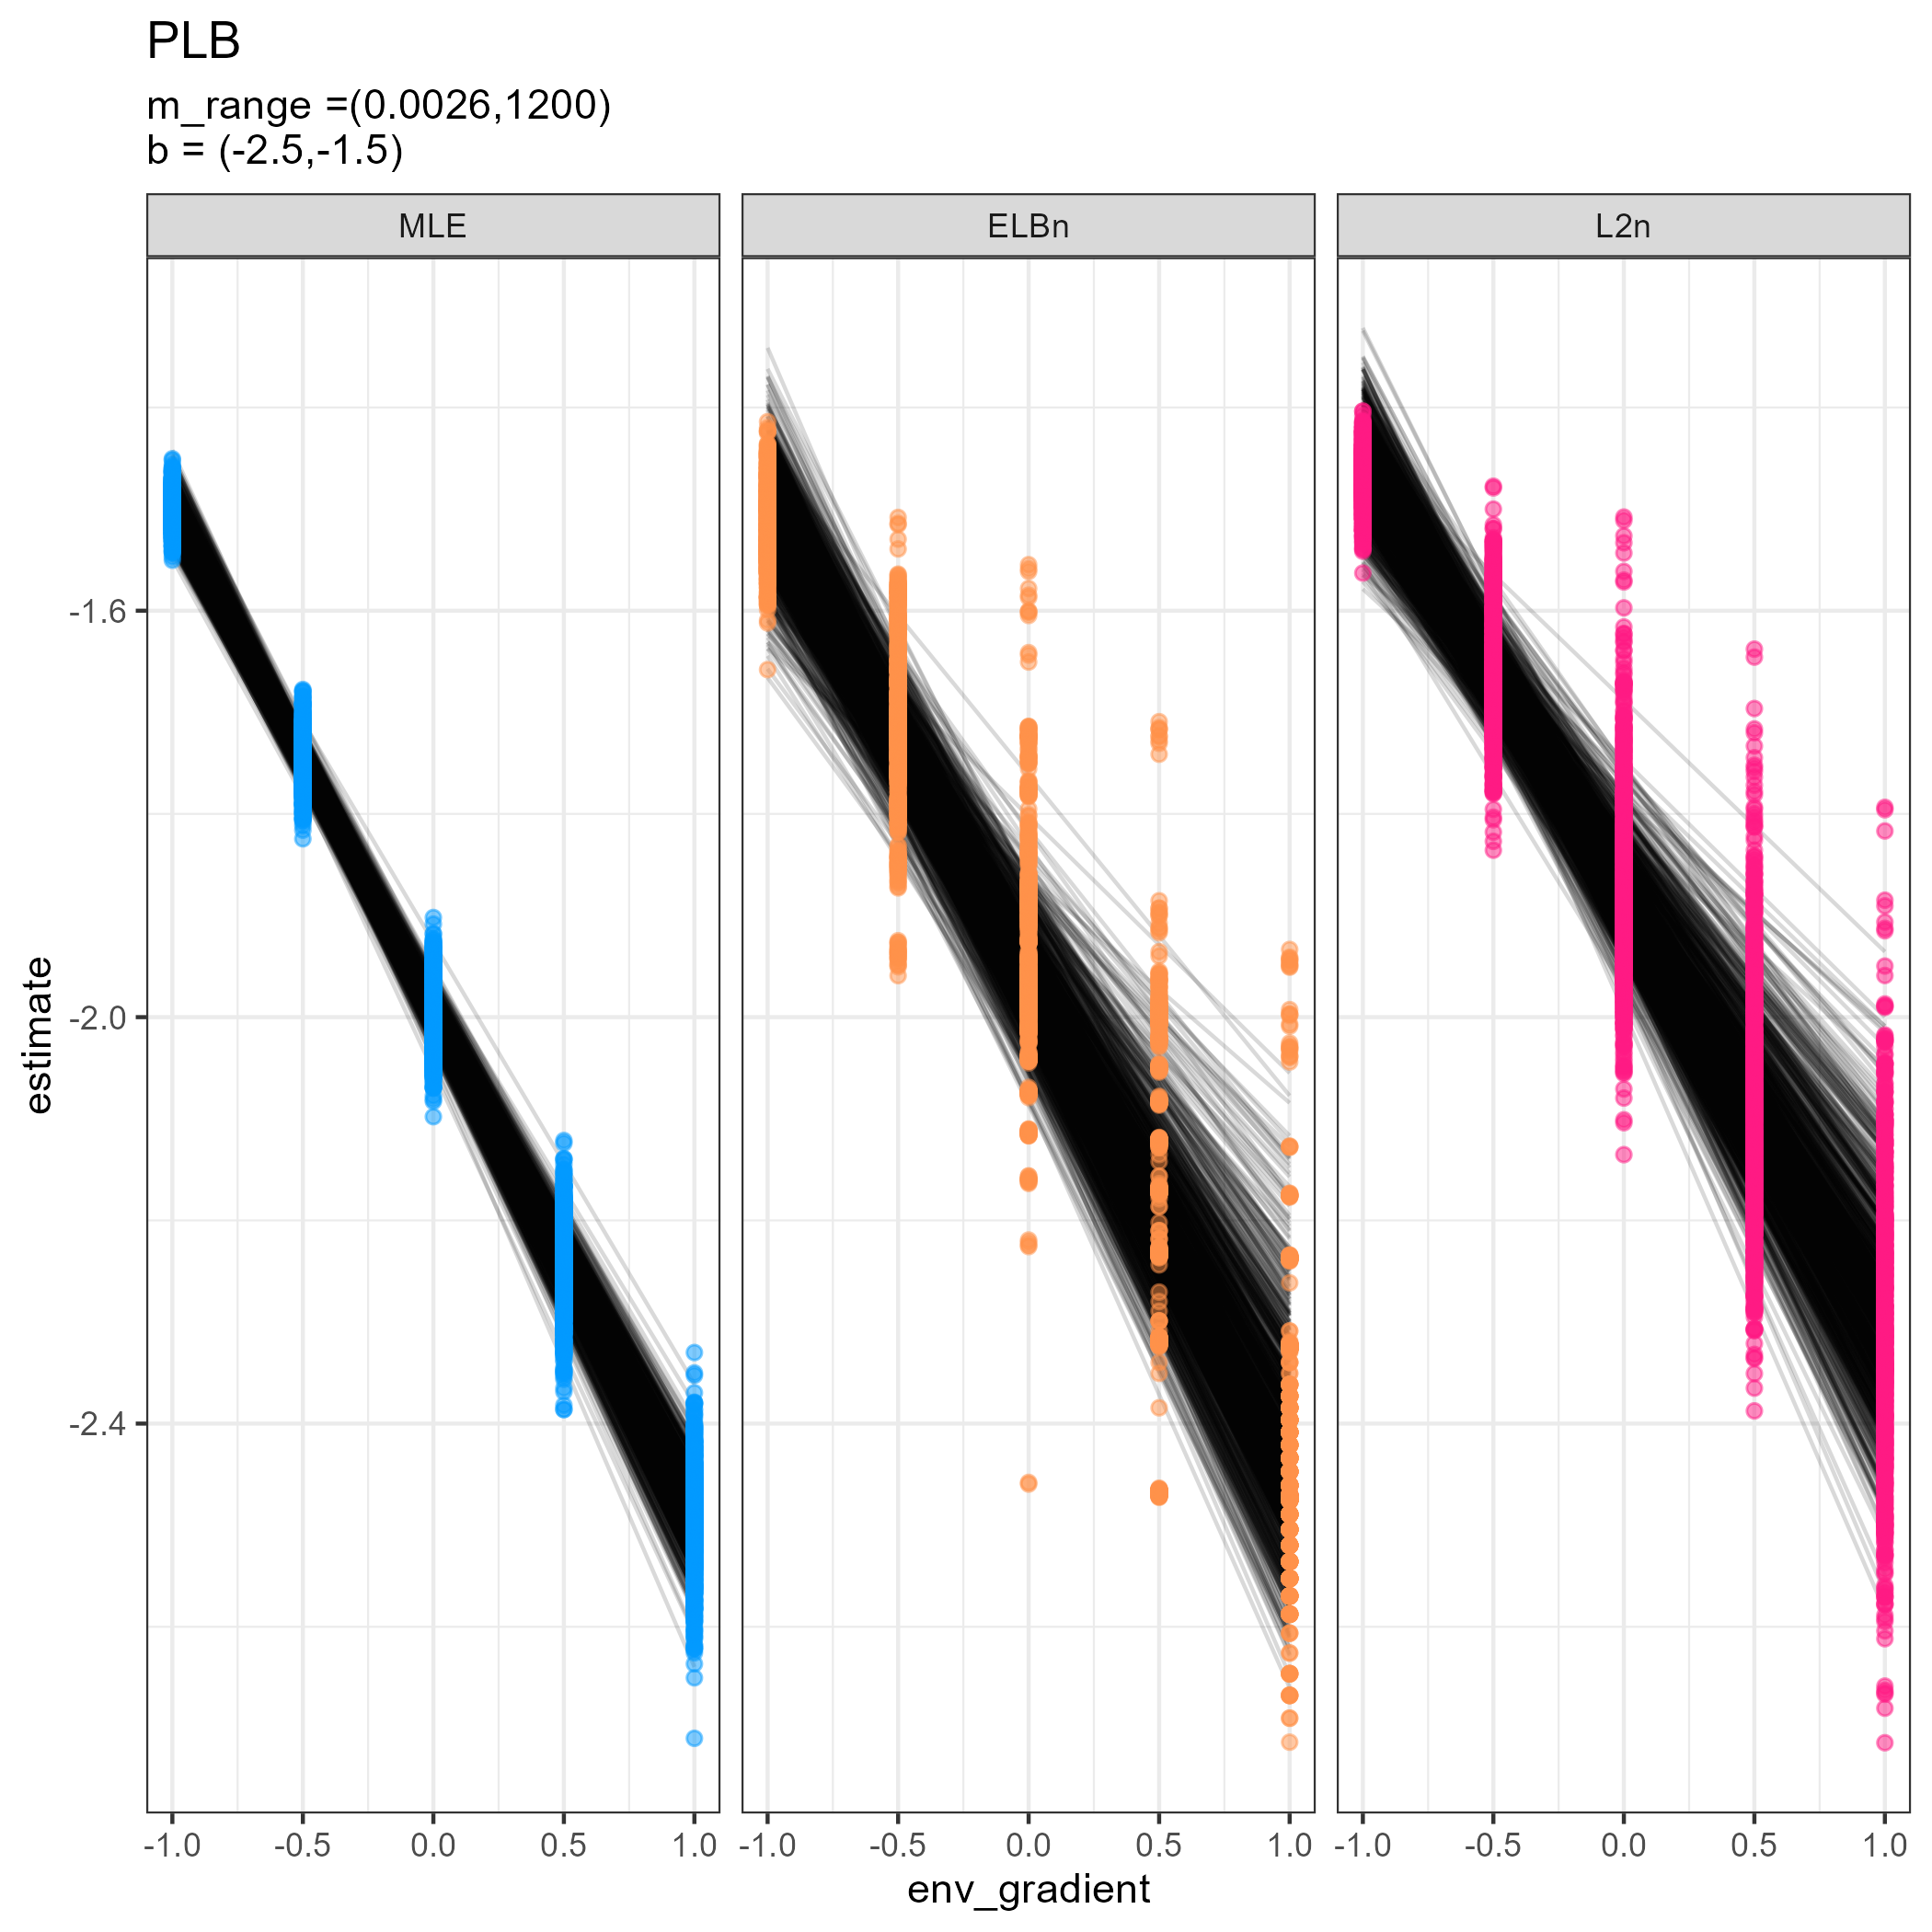
\includegraphics{figures/PLB_sim_main.png}
\caption{Relationship estimates across the hypothetical gradient for
each replicate. Each panel is a different method for estimating the size
spectra parameter.}
\end{figure}

\begin{figure}
\centering
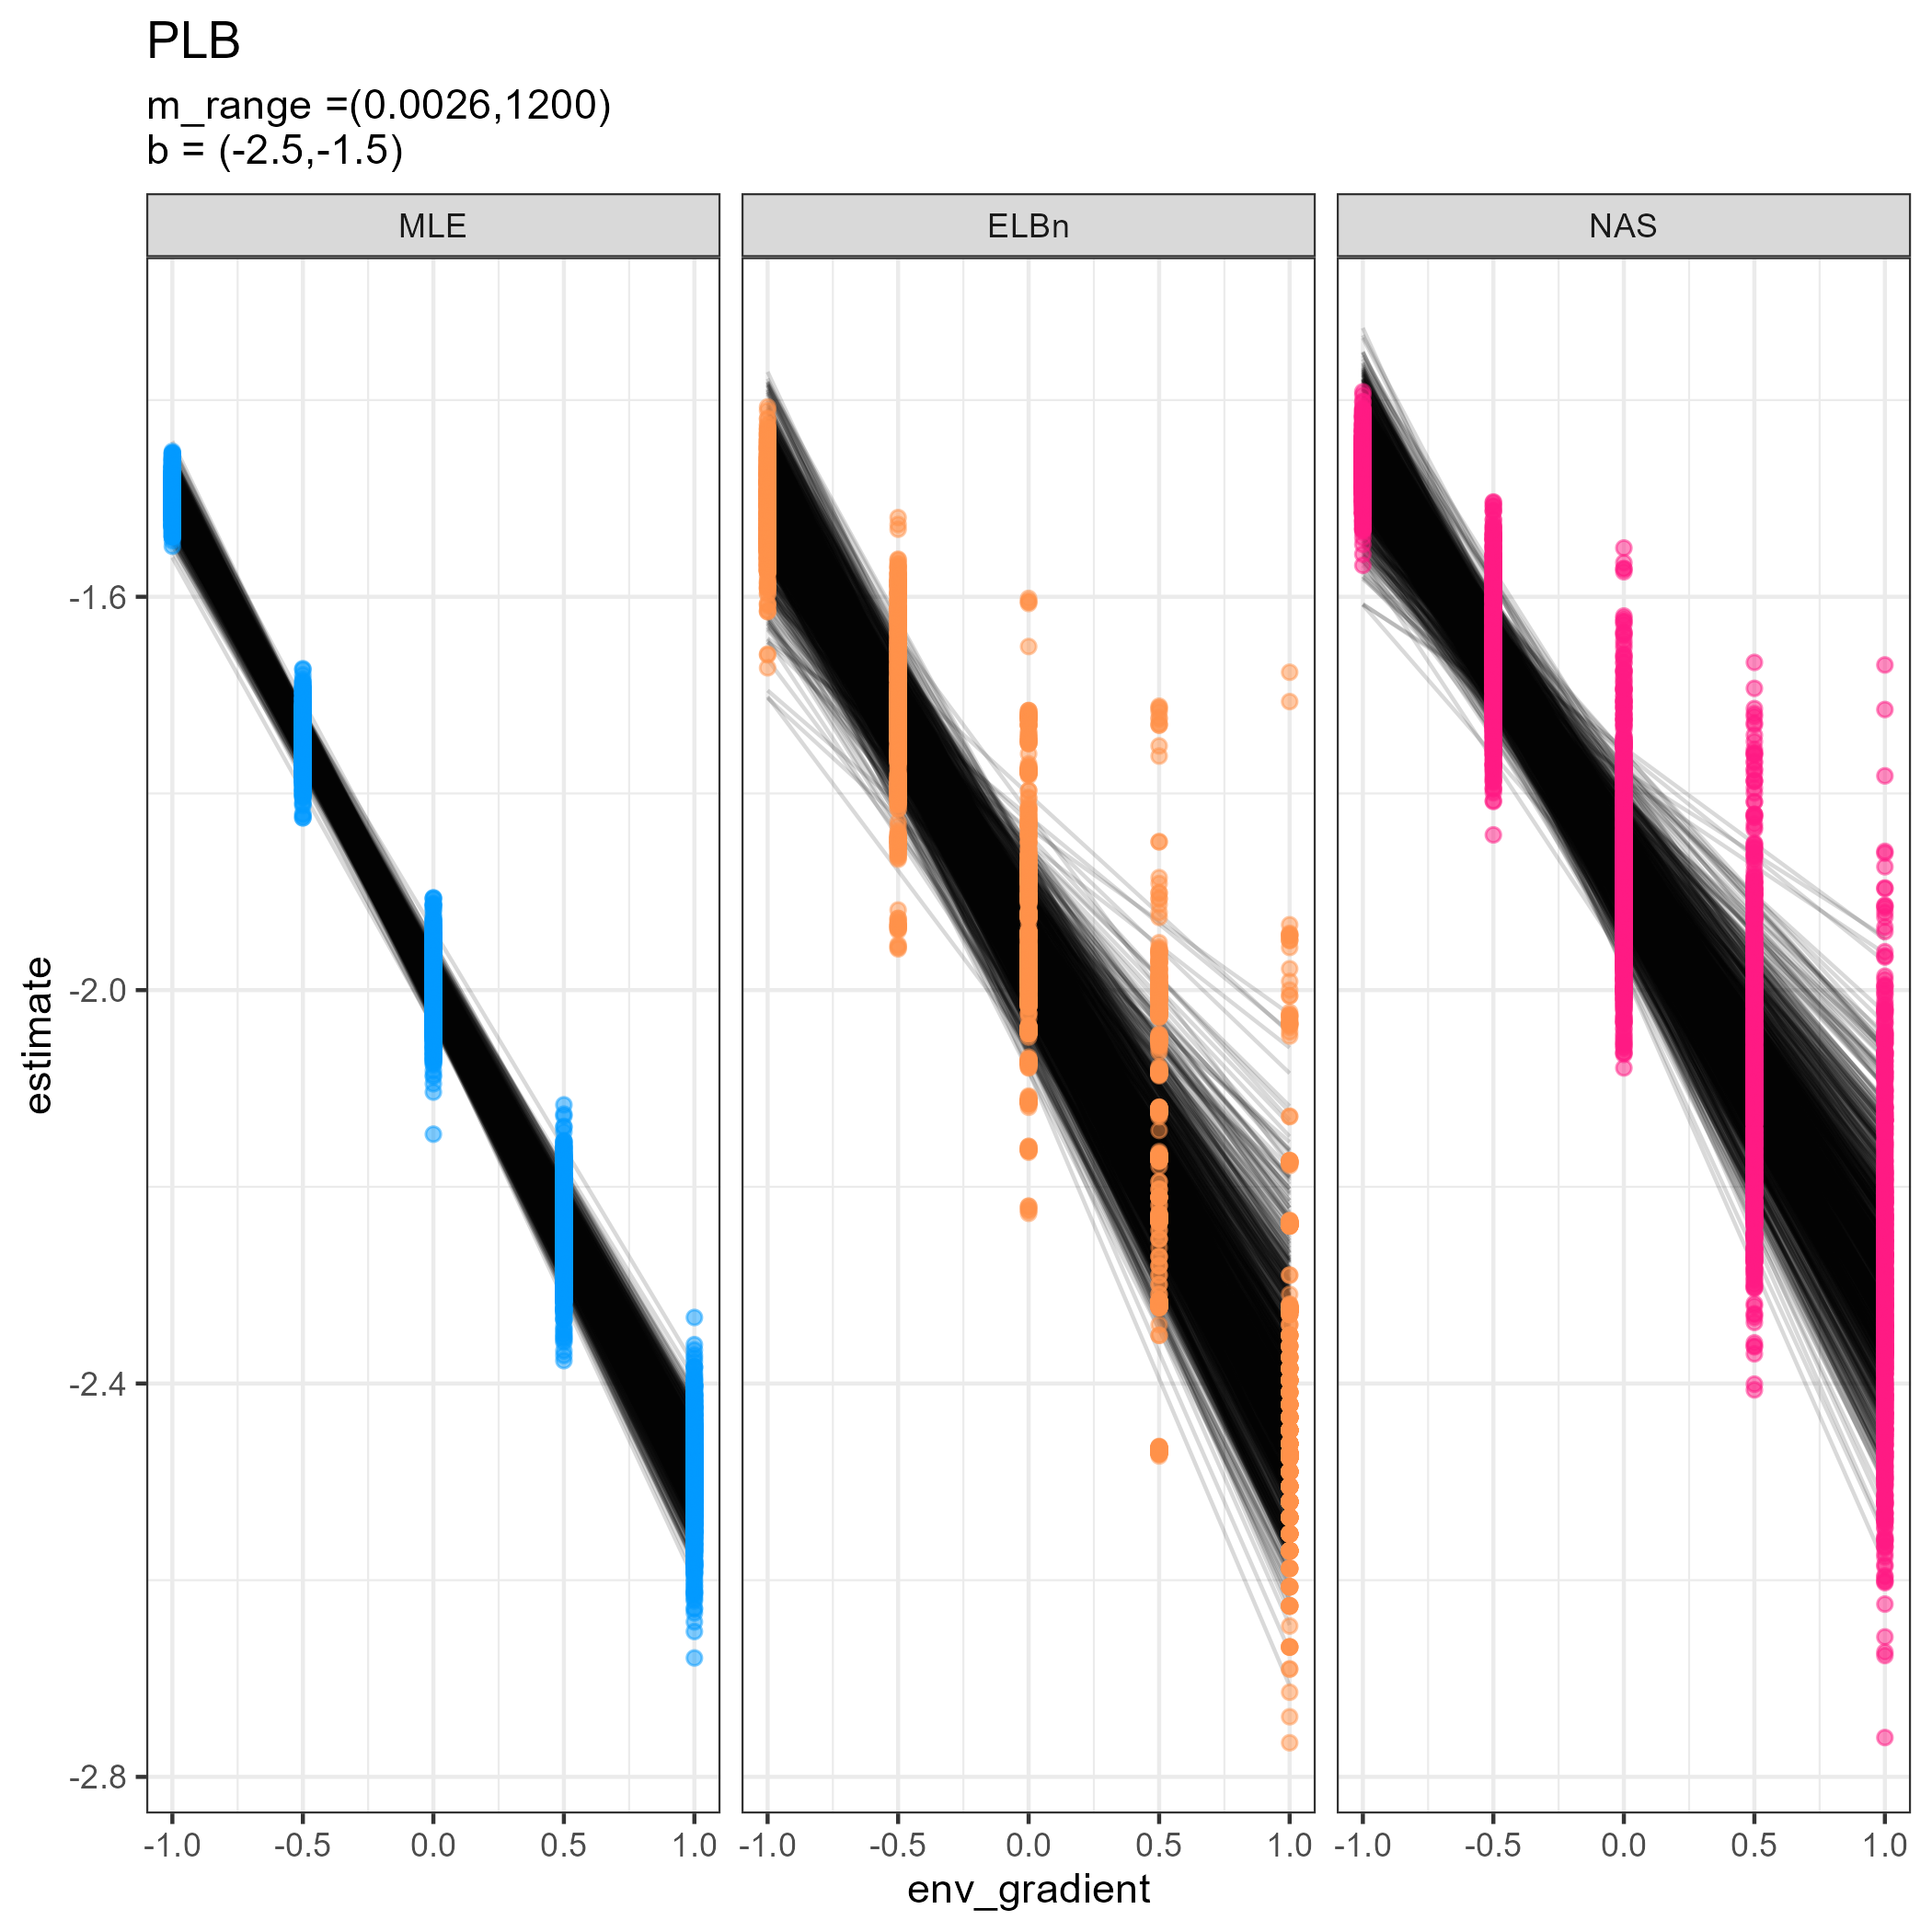
\includegraphics{figures/PLB_main_v2.png}
\caption{alternate plot version; I think I like this one better. What
are your thoughts on which you prefer??}
\end{figure}

The distribution of \(\beta_1\) estimates from MLE method were the most
accurate and precise, and the NAS method was the least accurate and
precise (Table \emph{xx}). The median estimates for all methods were
closer to the known relationship. All of the methods produced estimate
distributions with long right tails, but this pattern was greater in the
ELBn and NAS methods (e.g., SD for ELBn and NAS methods were 2-3x
larger, Figure \emph{xx} Halfeye plots).This result was consistent
across simulation parameters, including sample size, number of sites,
and \(\lambda\) values.

\newpage

\begin{figure}
\centering
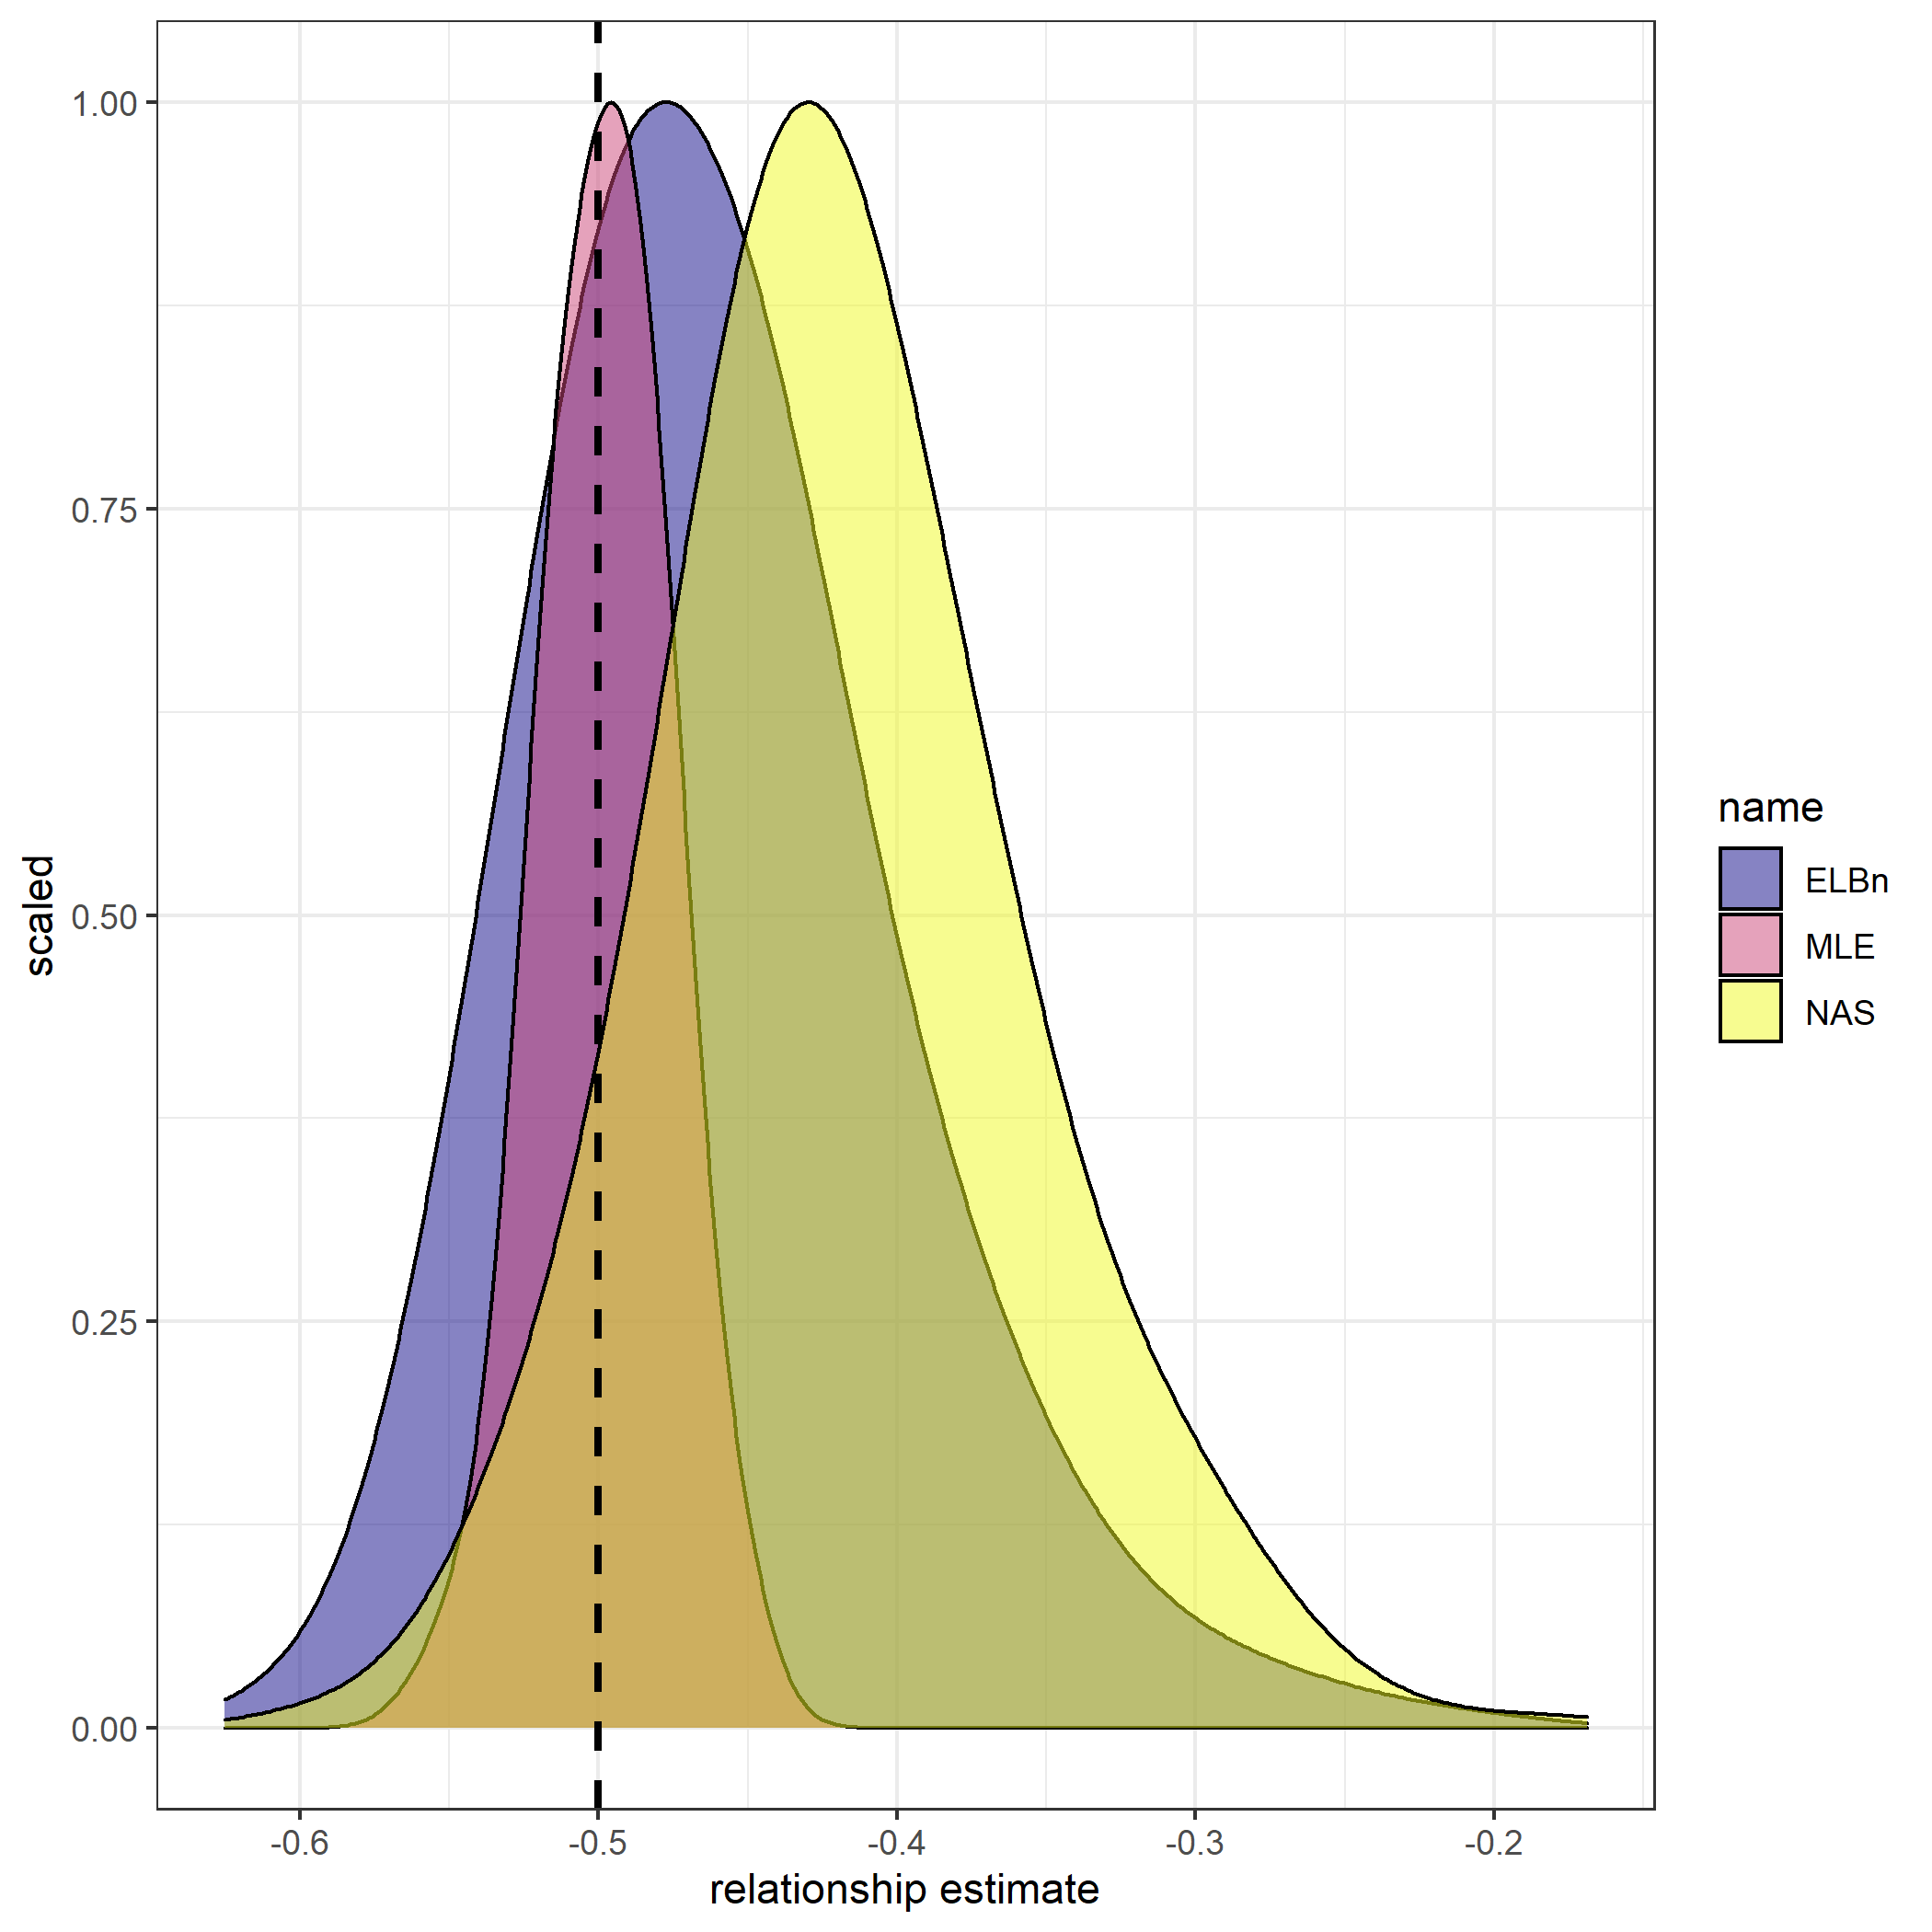
\includegraphics{figures/PLB_sim_relationship_density.png}
\caption{Halfeye plots for the estimated relationship coefficient
estimates across 1000 replicates and three different methods. The point
below each distribution plot is the median estimate, the thick and thin
bars represent the 66th and 95th percentile, respectively. Vertical line
is the known relationship. The median estimate for the MLE method was
closest to the known relationship, and had the narrowest distribution
across replicates.}
\end{figure}

\newpage

\begin{verbatim}
##   Model   mean    p50    p25   p975
## 1   MLE -0.495 -0.494 -0.499 -0.483
## 2  ELBn -0.460 -0.489 -0.524 -0.291
## 3   NAS -0.419 -0.442 -0.458 -0.302
\end{verbatim}

\begin{figure}
\centering
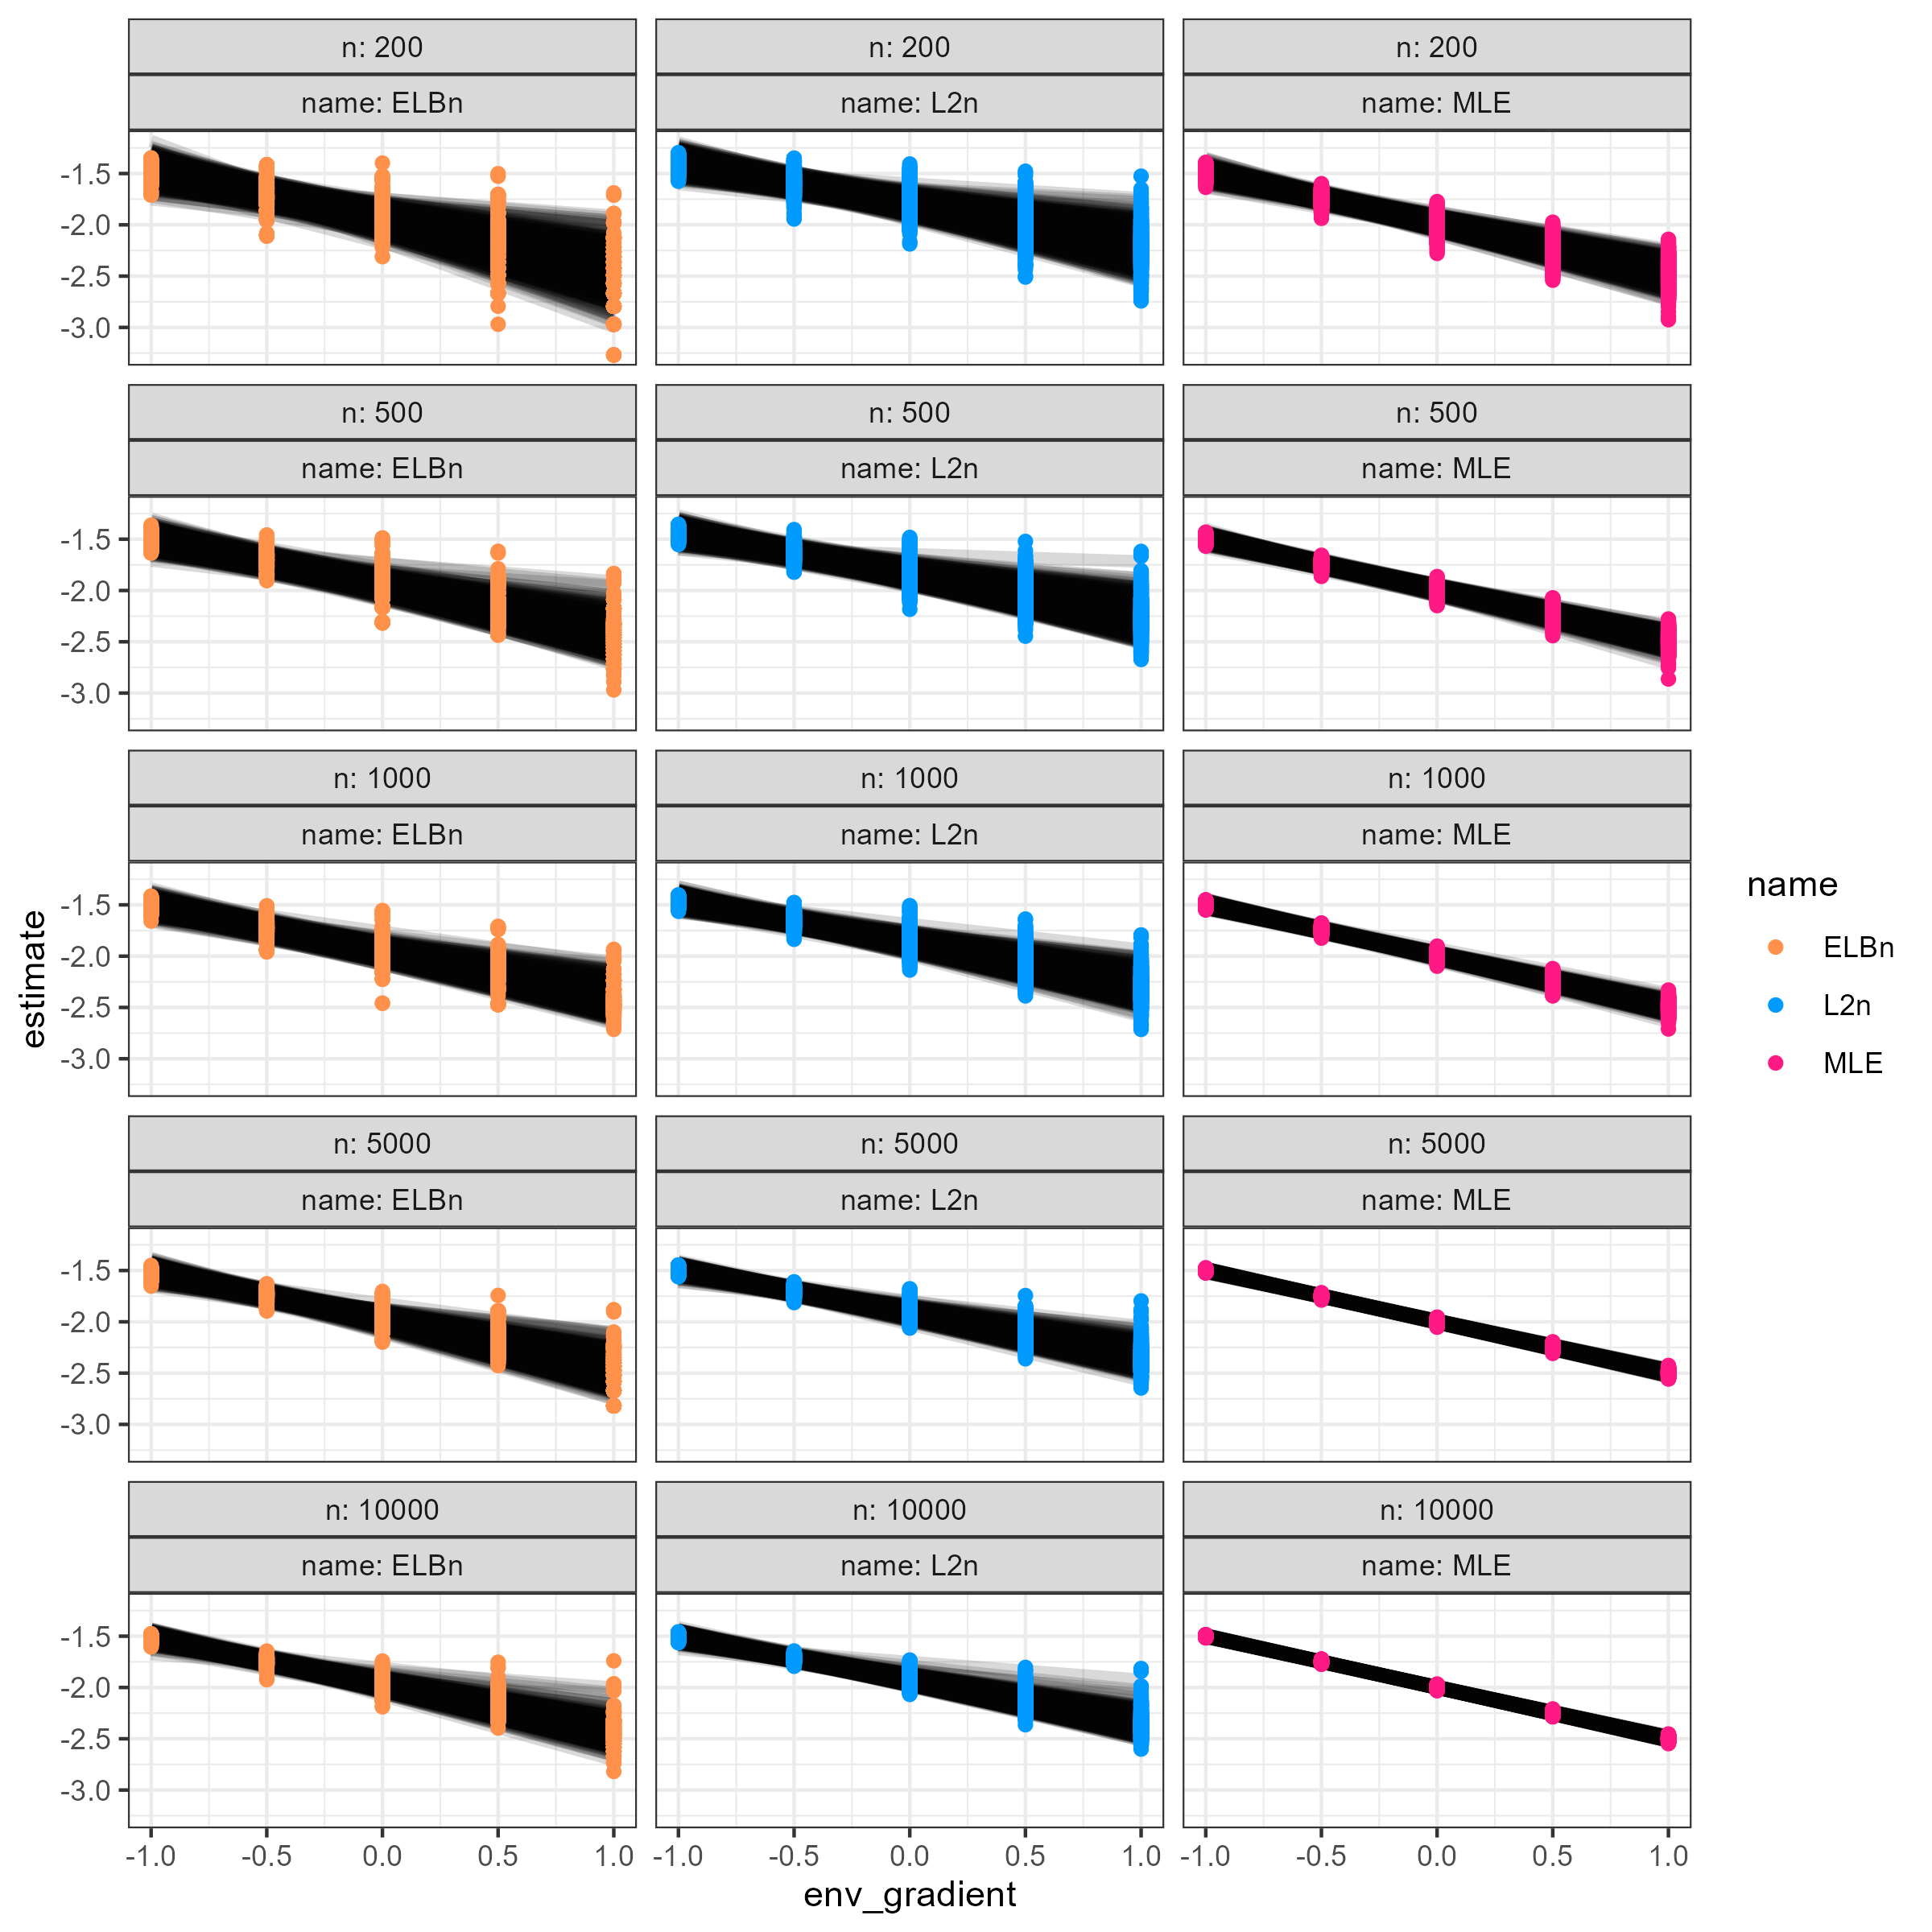
\includegraphics{figures/n_vary_main.png}
\caption{Individual regression estimates across the hypothetical
gradient based on sample size (rows) and methodology used (columns).
(match this figure to ``new'' style if we like that better)}
\end{figure}

\newpage

\hypertarget{no-relationship-1}{%
\subsection{No relationship}\label{no-relationship-1}}

All of the methods performed similarly when there was no relationship
across the hypothetical gradient. The mean \(\beta_1\) estimates for all
three methods ranged from -0.0005 to 0.0002. Although the distributions
were closely centered on 0, the distribution of coefficient estimates
was much wider for the two binning methods; the 95th percentile of the
MLE distributions is narrower than the 66th percentiles for the NAS and
ELBn methods.

\begin{figure}
\centering
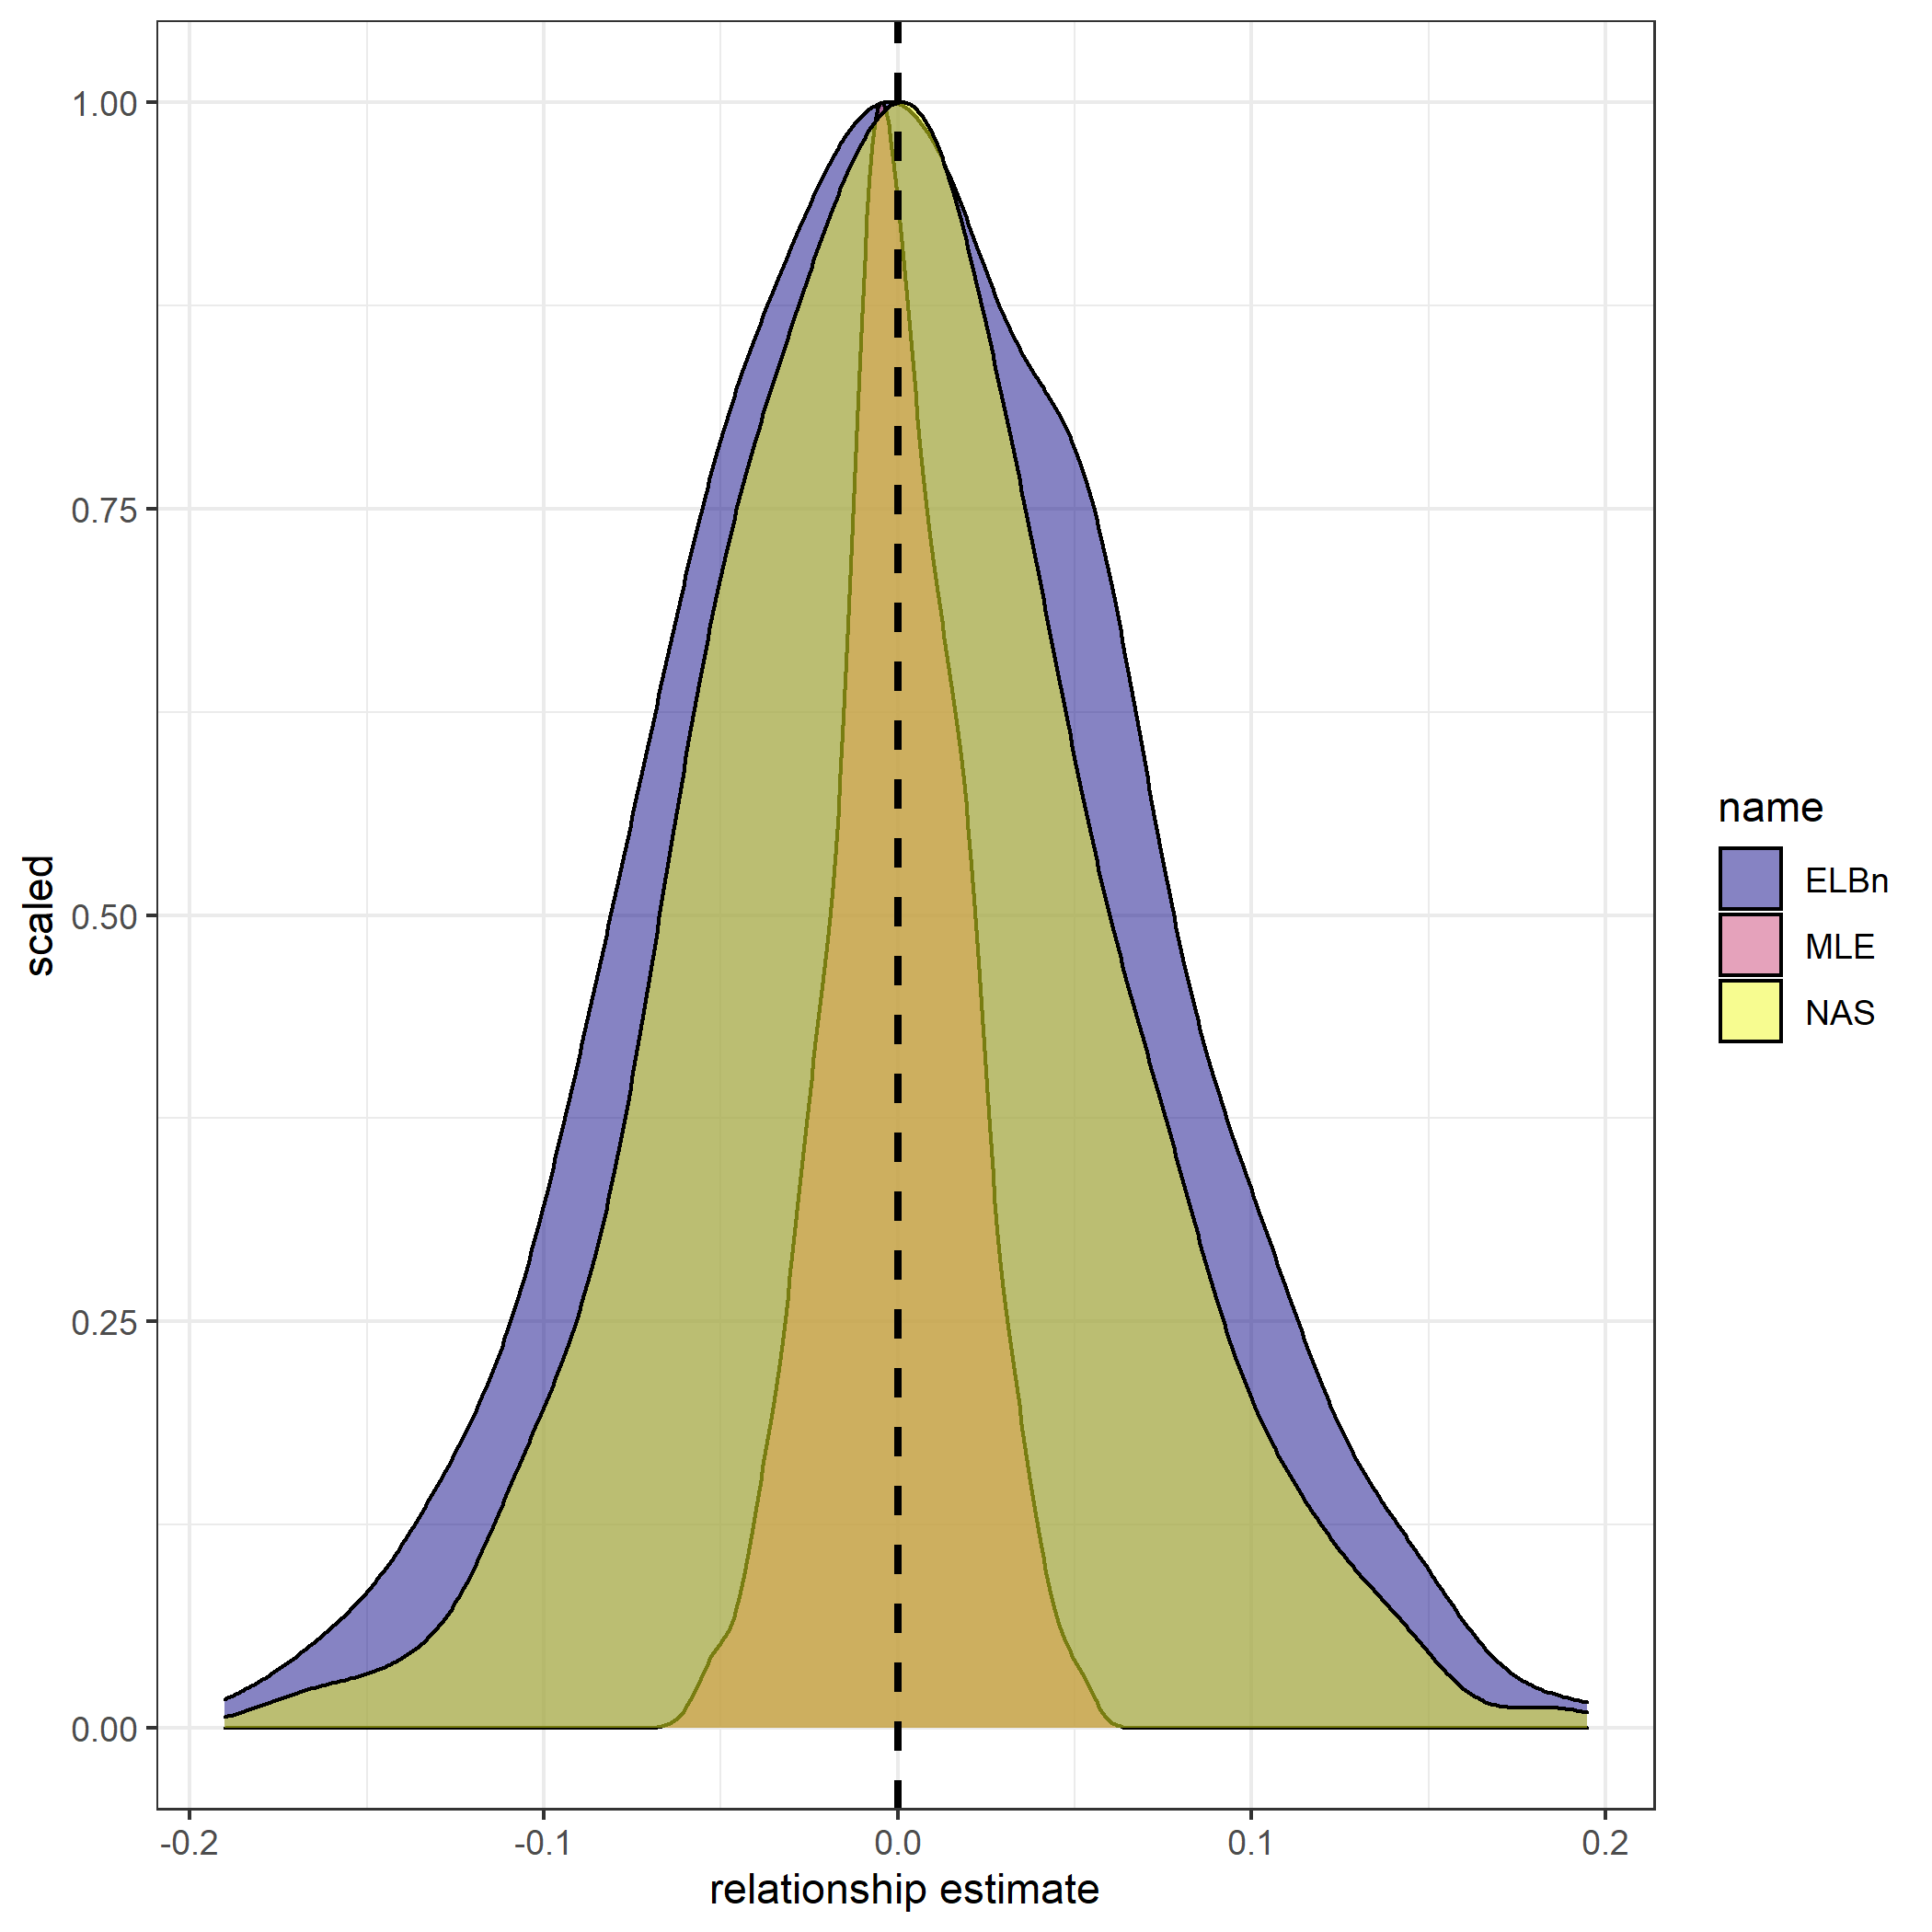
\includegraphics{figures/PLB_static_b_relationship_density.png}
\caption{Individual regression estimates when no relationship exists
across the hypothetical environmental gradient. The methods are
separated by rows. The median for all methocs is approximately zero, but
the distribution for the MLE method is narrower than the two binning
methods.}
\end{figure}

\begin{verbatim}
##   Model   mean    p50    p25  p975
## 1   MLE -0.001 -0.001 -0.012 0.038
## 2   NAS  0.000 -0.001 -0.039 0.119
## 3  ELBn  0.000 -0.001 -0.046 0.134
\end{verbatim}

\hypertarget{small-variation-in-lambda}{%
\subsection{Small variation in lambda}\label{small-variation-in-lambda}}

The performance of all methods to detect small variation in the
\(\lambda\) parameter (between -1.9 to -2.1) across the environmental
gradient was also investigated. The median \(\beta_1\) coefficient
estimates for the MLE method was -0.1, which exactly matched the value
for the hypothetical relationship, while the other two methods both had
median estimates of -0.09. The upper 97.5 percentile of the distribution
was below 0 for the MLE method, meaning that most of the estimates had
the correct sign. In contrast, the upper 97.5 percentile for both the
NAS and ELBn methods were greater than 0 at 0.027 and 0.052,
respectively. (Figure 4).

\begin{figure}
\centering
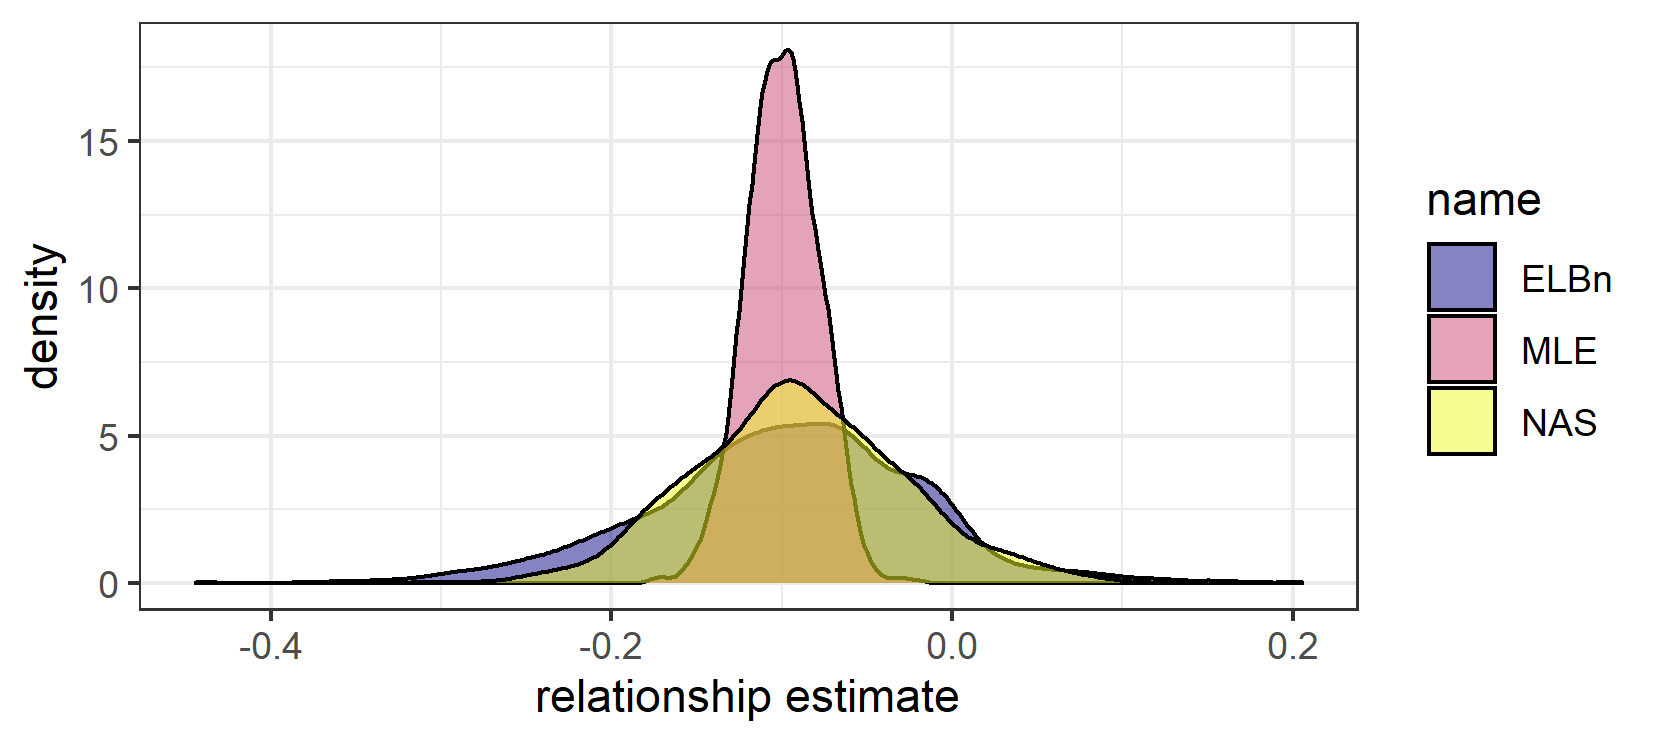
\includegraphics{figures/PLB_sim_small_relationship_density.png}
\caption{Distribution of the estimated relationship for each method.
Here, \(\lambda\) varied from -1.9 to -2.1, with a known relationaship
of -0.1 across the gradient indicated by the dashed vertical line. The
distribution of relationship estimates was approximately centered at the
known relationship for all methods, with a narrower distribution
observed for the MLE estimates.}
\end{figure}

\begin{verbatim}
##   Model   mean    p50    p25   p975
## 1   MLE -0.100 -0.101 -0.112 -0.062
## 2  ELBn -0.091 -0.095 -0.134  0.052
## 3   NAS -0.088 -0.091 -0.126  0.027
\end{verbatim}

\hypertarget{empirical-data-1}{%
\subsection{Empirical data}\label{empirical-data-1}}

For both empirical data sets, the direction and magnitude of change
(i.e.~\(\beta_1\) coefficients) are generally in agreement. Size spectra
parameters consistently increase (become flatter) in the AMD data (Fig.
XX A). Likewise, the size spectra parameters consistently increase
(become steeper) with increasing temperature across the NEON sites (Fig
XX D)

\newpage

\begin{figure}
\centering
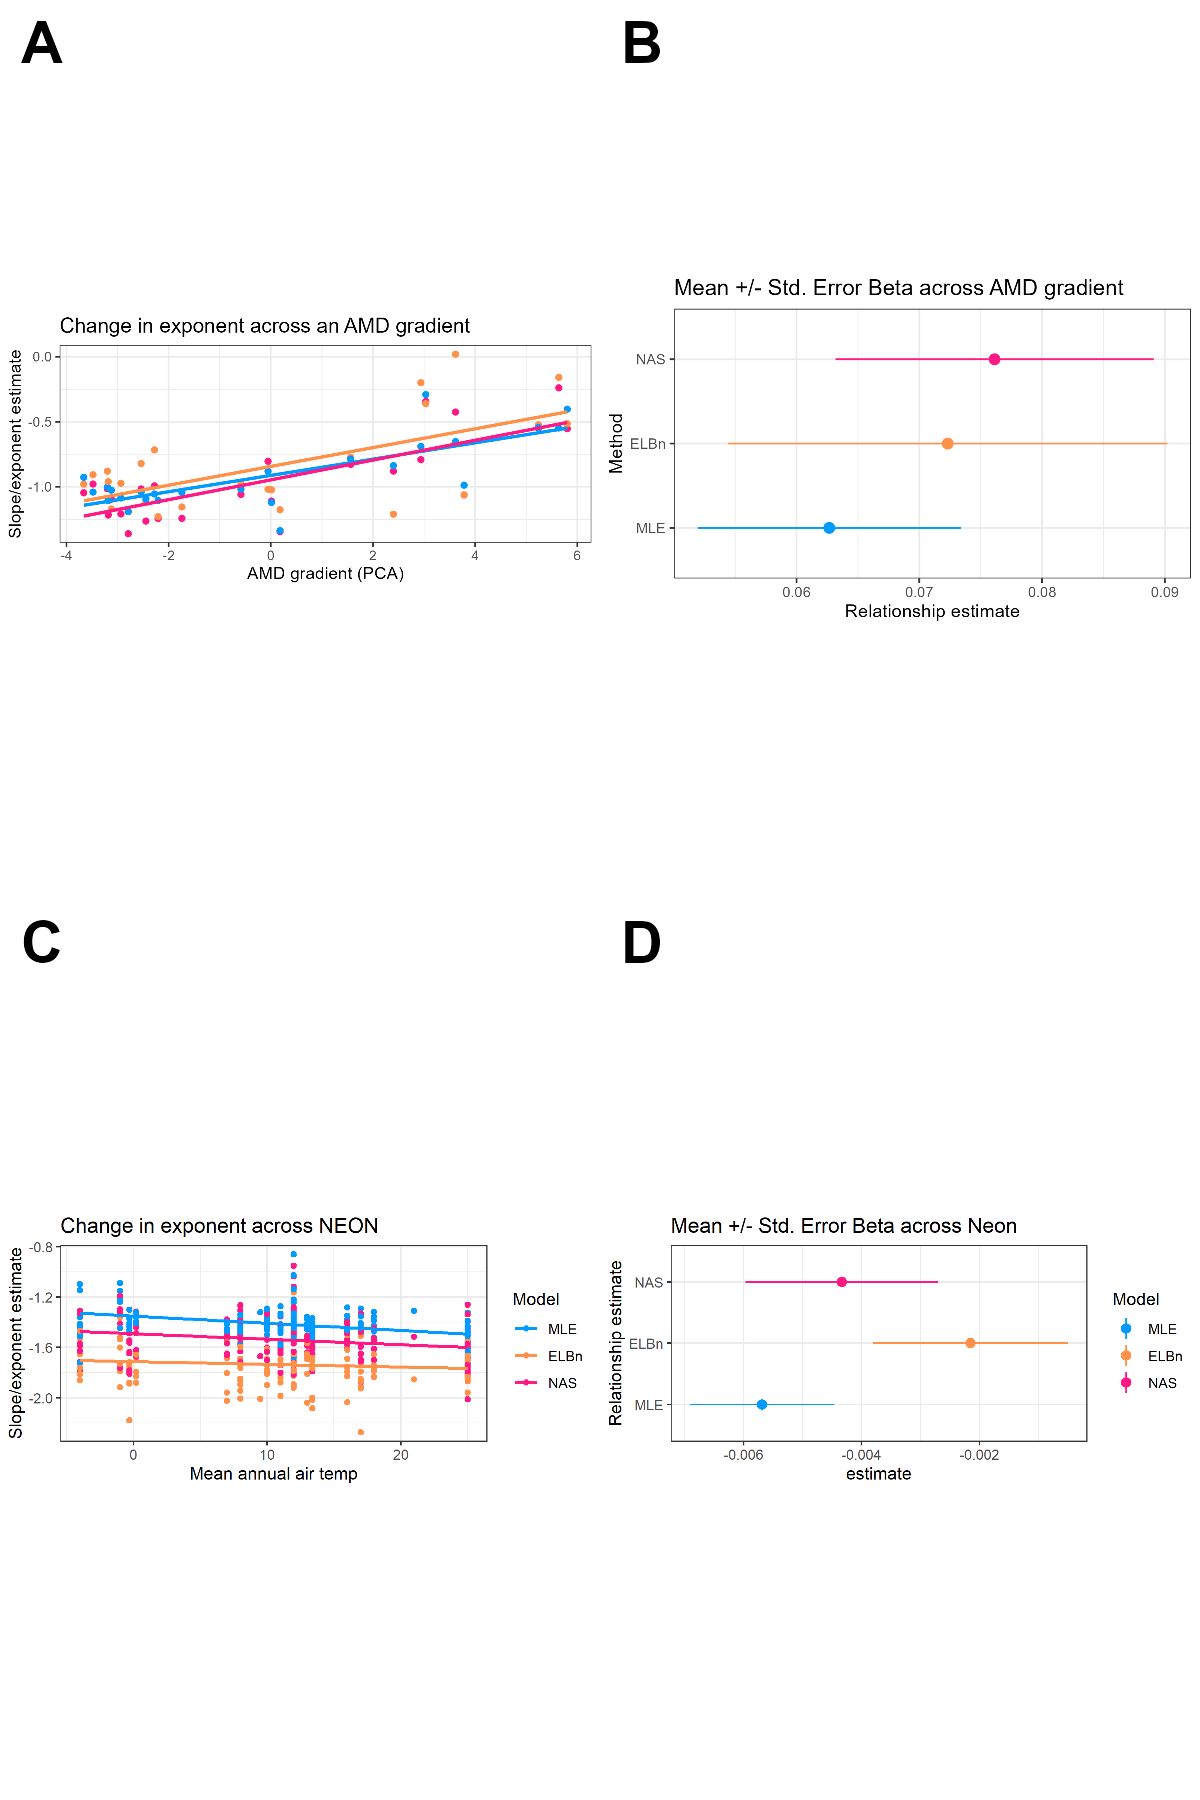
\includegraphics{figures/empirical_combined.png}
\caption{Figure of empirical data estimates. All of the methods estimate
the same sign of the relationship, but the estimates from the binning
methods are generally greater than the MLE estimates. \textbf{NOTE} I
need to re-plot these in ggplot and and stitch together. Currently
stitching pre-made png files, I think that's why it looks so funky.}
\end{figure}

\newpage

The \(\beta_1\) coefficient estimates for the AMD data are all positive
and of relatively similar magnitudes across methods. The MLE estimate
has the smallest magnitude and SD (0.063 \(\pm\) 0.011 SD), The ELBn
method is slightly larger and has a wider SD : (0.072 \(\pm\) 0.018).
Finally, the NAS method has the largest estimate and an intermediate
standard deviation (0.076 \(\pm\) 0.013). The range of the gradient in
the AMD data is relatively small (9.5), but the absolute change in the
size spectra parameter (\(\lambda\)) across the AMD gradient vary by
\textasciitilde0.13 units depending on the method used (range of
absolute change: 0.59 to 0.72).

Similar to the AMD results, the \(\beta_1\) coefficient estimates for
the NEON data are all negative and have similar magnitudes across
methods. The MLE estimate is once again the smallest (-0.006 \(\pm\)
0.001 SD). The NAS and ELBn methods are larger at -0.004 \(\pm\) 0.002,
and -0.002 \(\pm\) 0.002, respectively. Although the estimates are
similar and have a small magnitude, the range of the gradient in this
data is larger (\textasciitilde30\(\circ\)C), meaning that the absolute
change in \(\lambda\) estimates varies by 0.11 units depending on the
methods used (range of absolute change across gradient: 0.06 to 0.17).

\hypertarget{simulating-shallower-lambdas}{%
\subsection{Simulating shallower
lambdas}\label{simulating-shallower-lambdas}}

Estimates of the relationship between lambda and a hypothetical gradient
varied depending on the method used. However, interpretations of
empirical data were broadly consistent across methodologies. Upon closer
inspection, the values of size spectra parameters in the empirical data
were considerably shallower than -2. Given that we found the performance
of all methods increased with shallower \(\lambda\)'s we wanted to
investigate how the methods performed with simulated values closer to
the empirical estimates of parameters describing size spectra
relationships in streams. Therefore, we repeated the simulation process
as in the main analysis, but used \(\lambda\) values ranging from -1.1
to -1.5, with a known relationship of \(\beta_1 = -0.2\)

\newpage

\begin{figure}
\centering
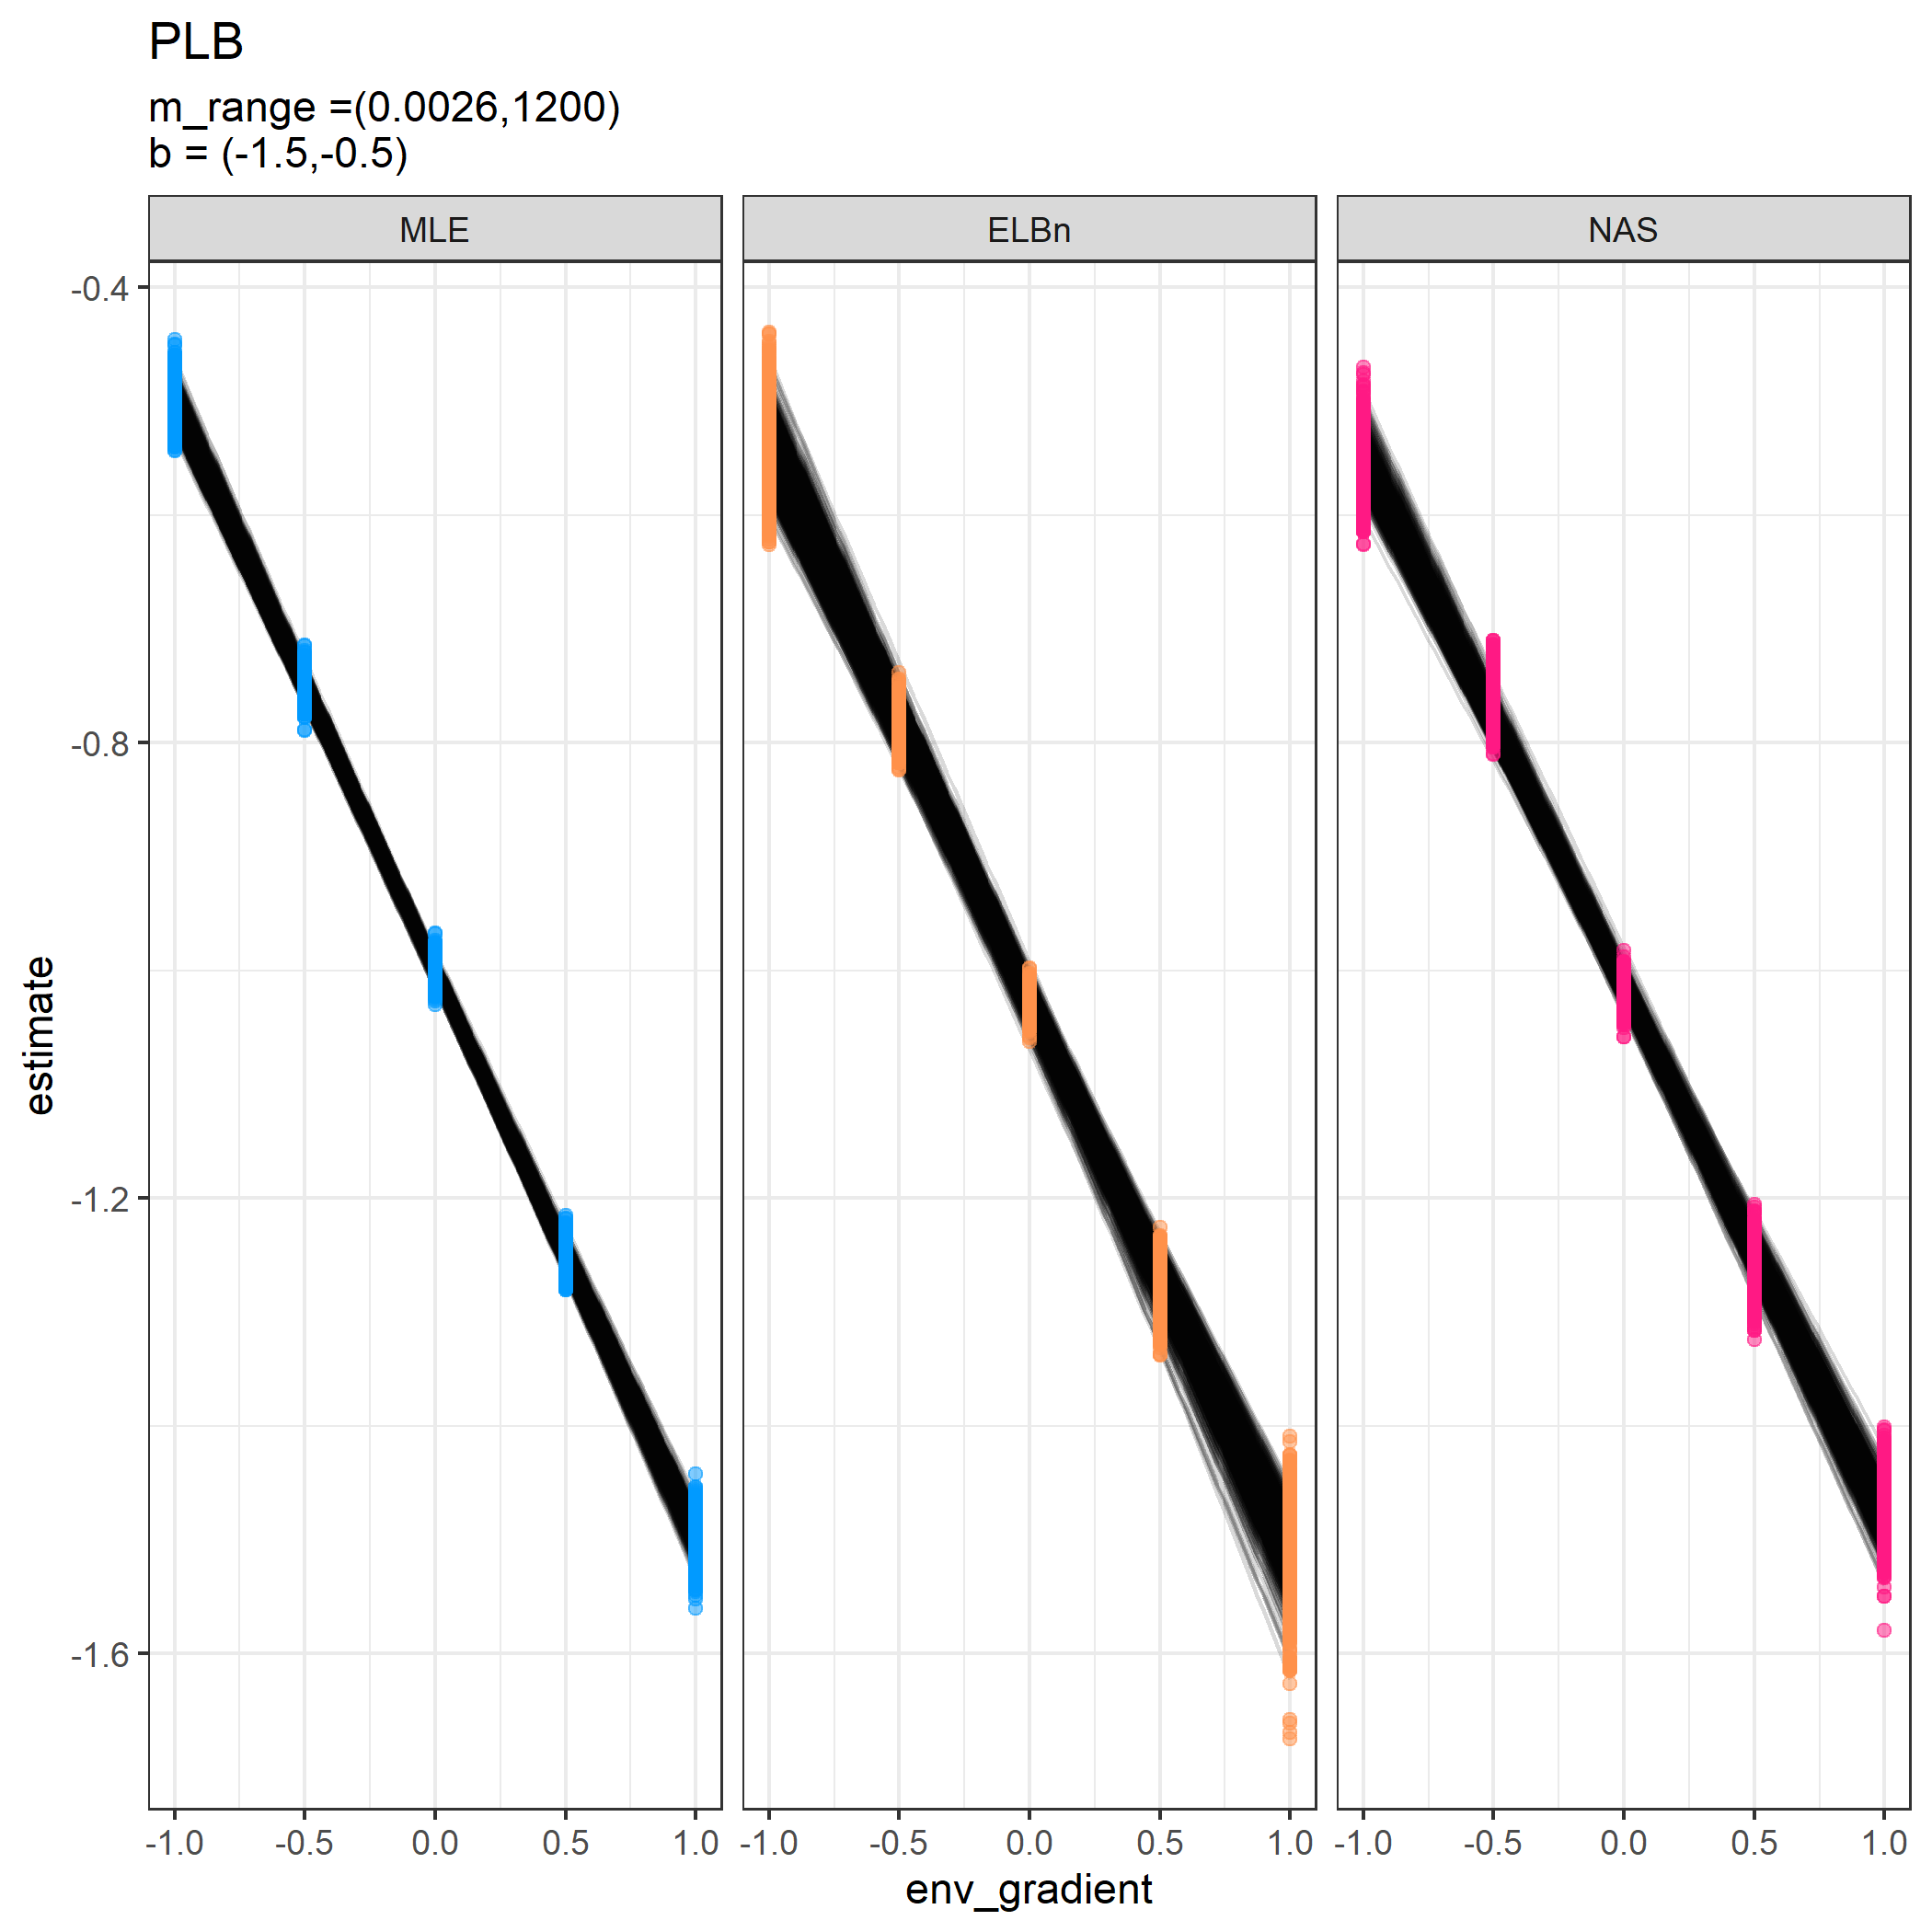
\includegraphics{figures/shallow_lambda_main.png}
\caption{Relationship estimates across the hypothetical gradient for
each replicate. Each panel is a different method for estimating the size
spectra parameter. (match to ``new'' style if needed)}
\end{figure}

We found generally less variability in the relationship estimates
(\(\beta_1\)) across a gradient of distributions described with
shallower \(\lambda\) parameters. However, the median MLE estimate was
once again closest to the hypothetical relationship and had the
narrowest distribution. The median ELBn estimate was close to the
hypothetical relationship but had a slightly wider distribution.
Finally, 95\% of the NAS estimates were greater than the hypothetical
relationship. In general, the distributions from the different
methodologies followed the same overall pattern, with the MLE estimates
being the smallest, and the binning methods being larger (i.e., more
positive).

\begin{figure}
\centering
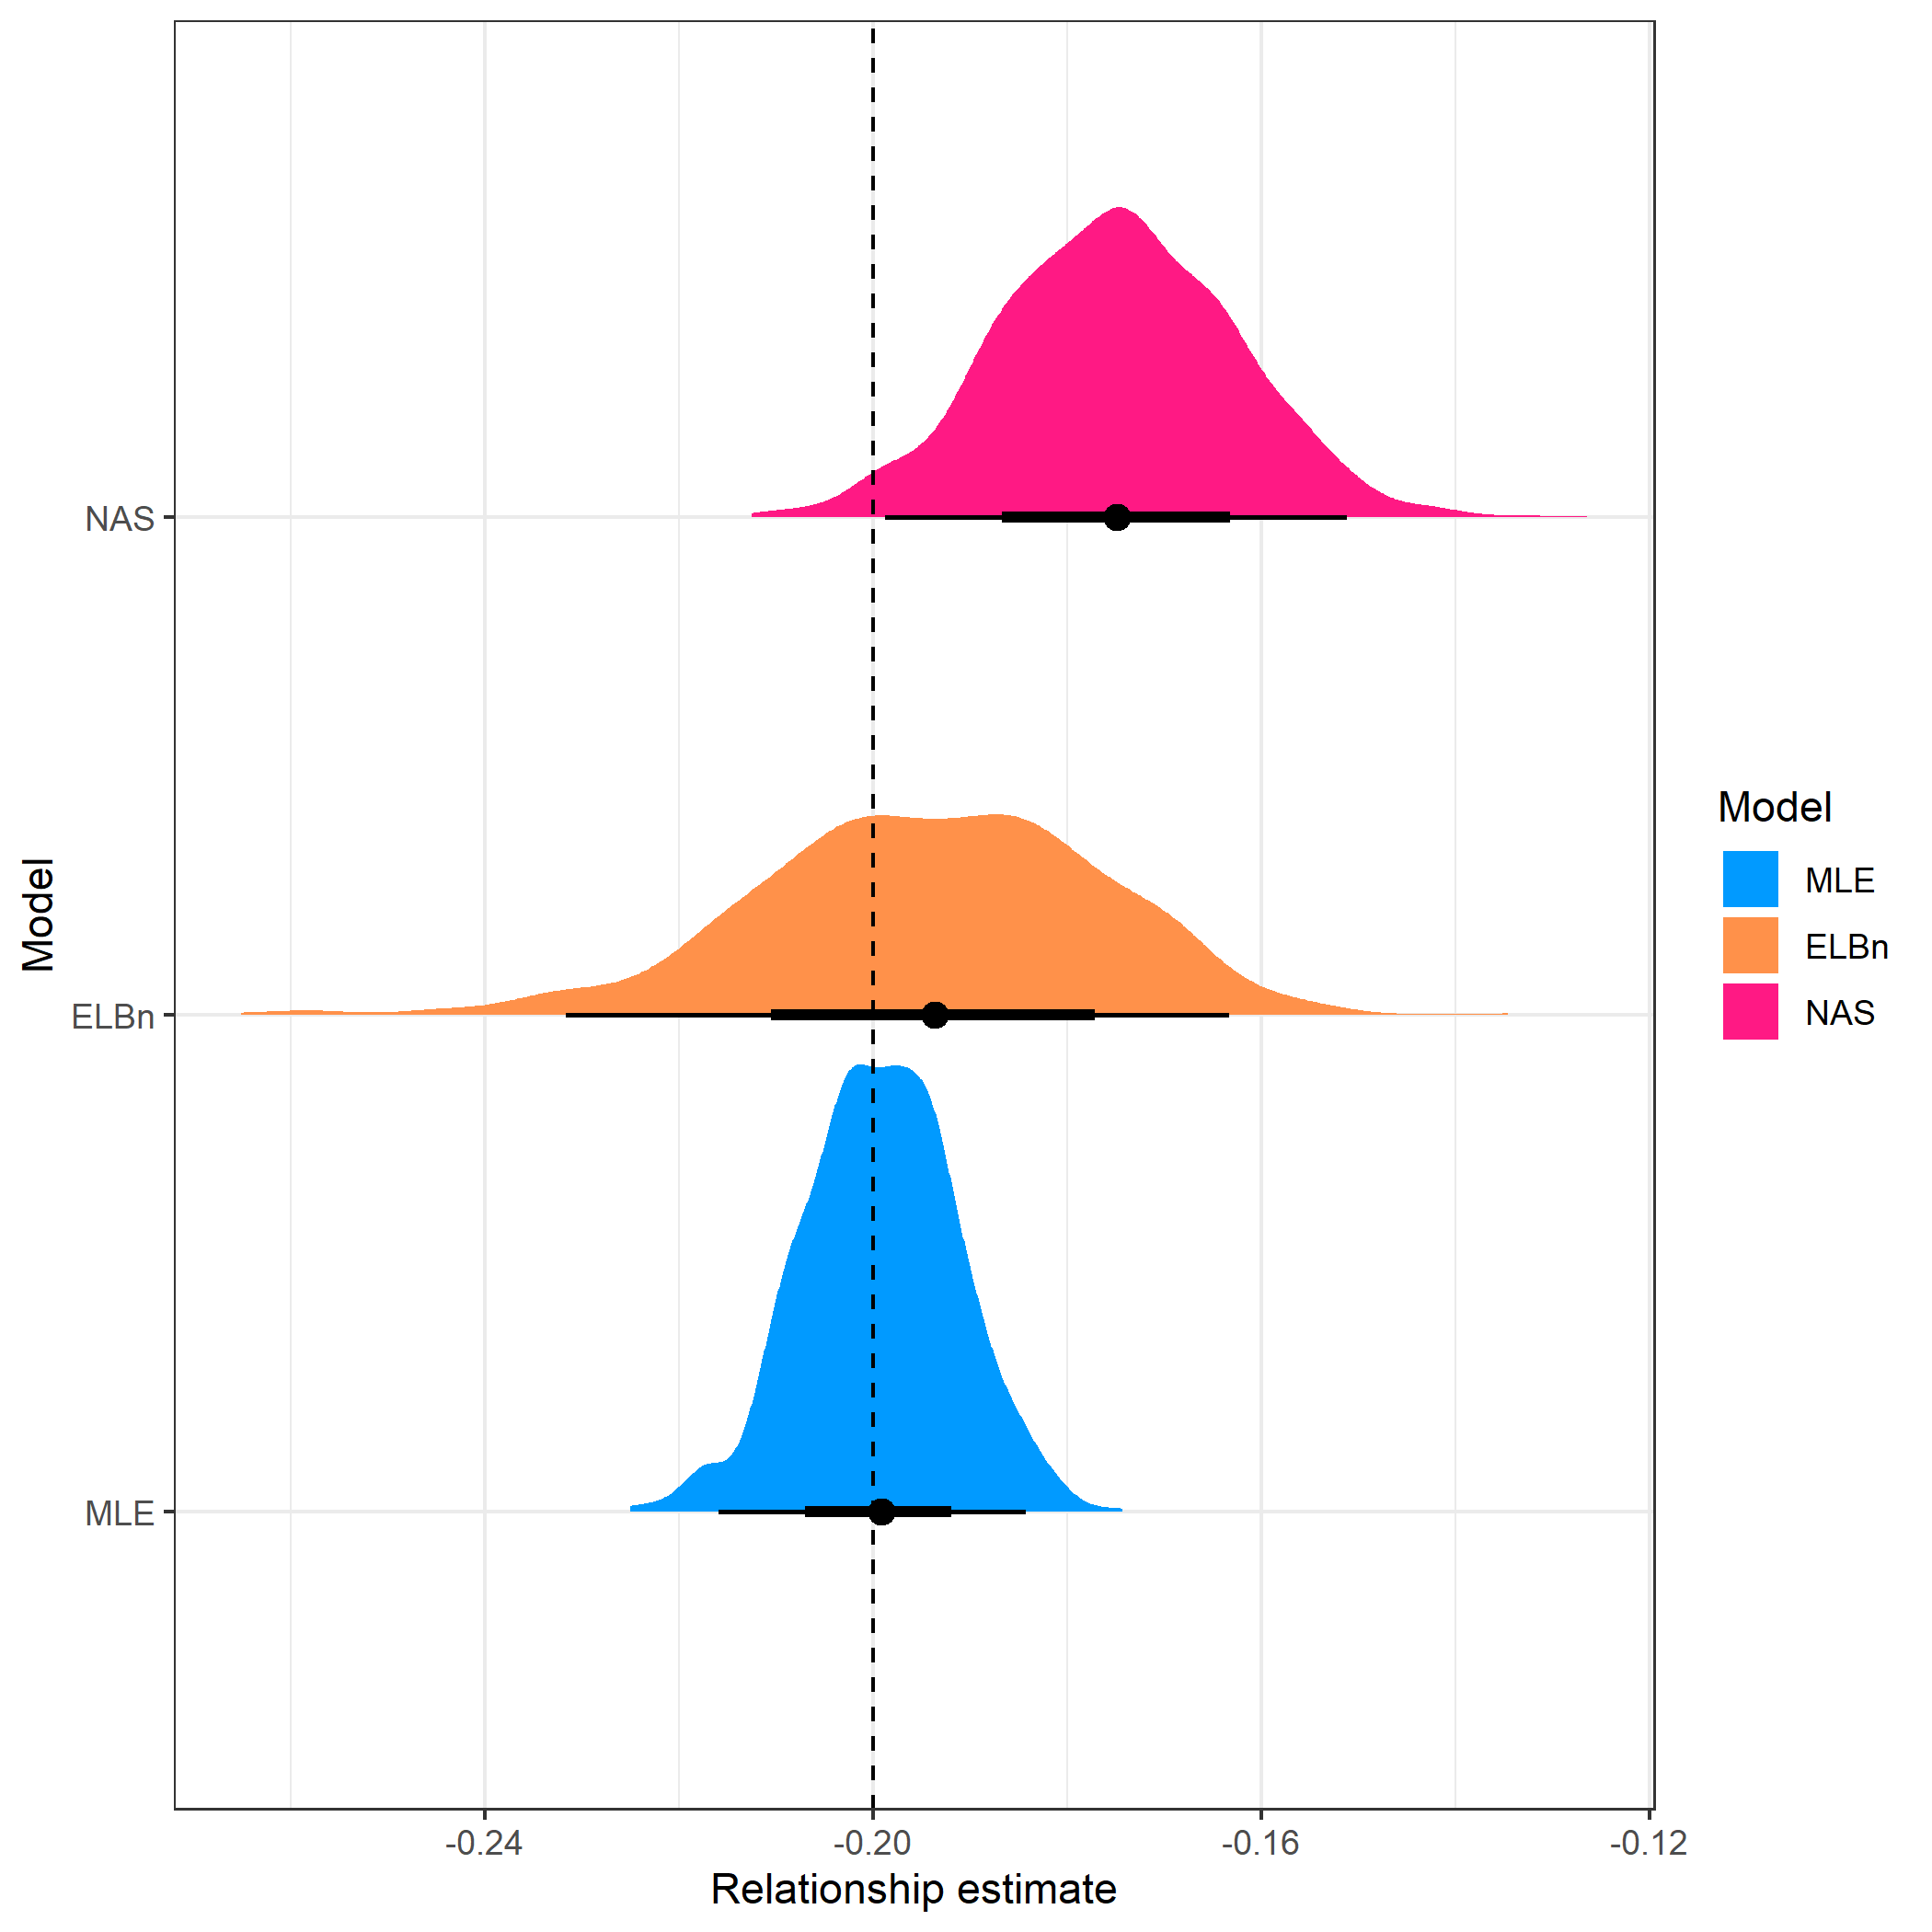
\includegraphics{figures/PLB_shallow_lambda_relationship_density.png}
\caption{Distribution of relationship coefficient estimates. Vertical
line is the known relationship. All methods under estimate the value,
but the mean magnitude and distribution of values is greater for the
ELBn and NAS methods. (not sure why this is such different proportions,
need to re plot with right dimensions)}
\end{figure}

\begin{verbatim}
##   Model   mean    p50    p25   p975
## 1   MLE -0.199 -0.199 -0.205 -0.183
## 2  ELBn -0.195 -0.195 -0.207 -0.161
## 3   NAS -0.174 -0.174 -0.183 -0.151
\end{verbatim}

\textbf{NOTE} Not sure if these tables are usful or not. Shows same
information as figures, but might be easier to see the quantitative
values instead of estimating from plot

\newpage

\hypertarget{discussion}{%
\section{Discussion}\label{discussion}}

Measuring parameters describing the decline in abundance with increasing
body size in communities is being done with increasing frequency across
ecology. Previous work has investigated the accuracy and inherent biases
associated with different estimation methods. However, how these
inaccuracies and biases compound across environmental gradients remains
uncertain, making it difficult to detect variation in size spectra
parameters across environmental gradients with confidence. Here, we
sampled body sizes from known distributions with varying parameters
(\(\lambda\)) and estimated the coefficient of the relationship
(\(\beta_1\)) across a hypothetical gradient in order to assess how the
results would vary depnding on the method used. Likewise, we compared
how the interpretation of previously published results could change
depending on the methodology used to estimate the relationship.

Generally, the estimate from the MLE method was always closer to the
known \(\lambda\) value, and resulted in the most accurate \(\beta_1\)
coefficient estimate for the hypothetical relationship in simulated
data, and always had the smallest variation around the estimate.

Binning methods are easy to use and interpret, which most likely
accounts for their wide use in ecological studies. However, aggregating
individuals into logarithmic bins removes a large source of the
variation within the data by collapsing body size variation into a
single values within bins. For example, all individuals placed into a
bin that ranges from 2-4 grams of mass are all treated as having a mass
of 3 grams, the midpoint of that bin. Likewise, a single abundance value
is taken for this bin, despite that fact that there is almost certainly
variation in the abundance of individuals that weigh \textasciitilde2
grams or \textasciitilde4 grams. By homogenizing the data in this way,
it seems that binning methods will always produce noisier results than
MLE from the binning process alone, since binning is akin to deleting
information that the model could otherwise use. One of the benefits of
using MLE is that all data points are retained for use within the model.

The variation in estimated relationships across the empirical datasets
varied by \textasciitilde0.1 units depending on the method used. At
first glance this may not appear to be a concerning magnitude of
variation. However, when one considers the range of variation reported
in many seminal works on size spectra relationships in streams is
\textasciitilde0.1-0.2 (SI Table \emph{xx}), it is apparent that many of
these results may be dependent on the method used.

The performance of all methods improved as sample size increases, and as
the exponent of the size spectra relationship gets larger (more
shallow). As either or both of these variables change, the difference in
estimated relationship coefficients declines across the methods. This is
particularly interesting given the fact that both empirical data sets of
stream communities examined here are shallower than the expected
relationship of \(\lambda = -2\), and the conclusions of the change in
size spectra relationships across the gradients are not dependent on
method used. If communities under study are in fact described by
shallower exponents, the method used may not be critical in the
conclusions reached. However, the MLE method performs as well or better
than the two binning methods examined here under all contexts and should
be the preferred method in future studies. At a minimum, future studies
should report MLE estimates to ensure that the results are not dependent
on the methodology used.

Despite the drop in performance with reduced variation in \(\lambda\)
values, the estimated relationship coefficient was generally in the
correct direction and of a similar magnitude. This suggests that
previously reported significant changes in size spectra parameters
across environmental gradients and in experimental manipulations are
plausible. Given that all of the data within a study is treated
identically, the the over all change in size spectra parameters is
likely reasonable. However, the biases and inconsistencies in
relationship estimates presented here suggest that it would be difficult
if not impossible to compare the relative changes across different
published studies which use different methods. Publication of individual
body size data with future studies of size spectra relationships would
greatly aid in our ability to generalize changes to this fundamental
aspect of community organization across spatiotemporal scales and in
response to environmental conditions.

\textbf{NOTE} not sure if the idea below belongs in this paper or not,
but it's something I've been thinking about for a while. I'm using this
as an excuse to write out my thoughts and to see what y'all think about
it. Maybe it's another paper to write in the future?

An interesting finding is that the empirical data sets used here were
quite a bit shallower than is expected based on theory, and that what
has been observed empirically in marine systems. There are two,
non-mutually exclusive, possible explanations for this: 1) freshwater
streams are more dependent on detrital resources, 2) streams are
effectively 2D systems, whereas marine systems are 3D. Blanchard et
al.~(2009) observed that benthic marine communities had shallower slopes
than pelagic communities, and that this was likely due to a stronger
reliance on a shared detrital basal resource in the benthic community,
whereas the pelagic community was largely driven by energy transfer
through predator-prey interactions. The importance of allochthonous
resources in stream ecosystems has long been recognized (Vannote et
al.~1980). The stream data here largely comes from low order, headwater
streams which may be reasonably considered to be driven by allochthonous
resources. It is possible that the communities sampled here are
structured based on a shared basal resource, and that the importance of
predator-prey interactions is reduced. An alternate hypothesis is the
relative dimensionality of search space in benthic and pelagic systems.
Consumption rates and interaction strenghts have been shown to vary
markedly based on search dimensionality. Consumers generally encounter
resources more frequently in 3D environments (i.e., aerial, pelagic)
than in 2D environments (i.e., benthic, terrestrial), and lead to
stronger consumption rates and interaction strengths. Likewise, it has
been hypothesized that the scaling exponent for mass-specific search
rates may vary based on search space dimensionality instead of being set
at approximately 0.75 (Pawar, Dell, Savage, 2012).

\hypertarget{concluding-remarks}{%
\subsection{Concluding Remarks}\label{concluding-remarks}}

Both of the binning methods can perform as well as MLE under certain
circumstances (large sample size, shallow \(\lambda\)). However, it
would be unlikely for a researcher to know if this was the case
beforehand. Furthermore, in order to confirm this result, MLE methods
would likely need to be employed. With the publication of the
\emph{sizespectra} package (2017), producing MLE estimates of size
spectra parameters is a relatively easy task. Therefore, we recommend
using this in all future studies of size spectra relationships.

We reiterate the recommendations of White et al.~(2007)(2007), Sprules
and Barth (2016)(2016) and Edwards et al.~(2017)(2017) to estimate size
spectra relationships using MLE methods due to their superior
performance in nearly every context. Furthermore, we strongly encourage
authors to publish individual size data whenever possible. This will
allow for the consistent re-analysis of existing data sets as
methodologies develop and improve. This will aid in the ability for size
spectra work to be synthesized between research groups and across
scales.

\newpage

\hypertarget{references}{%
\section{References}\label{references}}

\hypertarget{refs}{}
\begin{CSLReferences}{1}{0}
\leavevmode\vadjust pre{\hypertarget{ref-edwards2020}{}}%
Edwards, A. M., J. P. W. Robinson, J. L. Blanchard, J. K. Baum, and M.
J. Plank. 2020. \href{https://doi.org/10.3354/meps13230}{Accounting for
the bin structure of data removes bias when fitting size spectra}.
Marine Ecology Progress Series 636:19--33.

\leavevmode\vadjust pre{\hypertarget{ref-edwards2017}{}}%
Edwards, A. M., J. P. W. Robinson, M. J. Plank, J. K. Baum, and J. L.
Blanchard. 2017. \href{https://doi.org/10.1111/2041-210X.12641}{Testing
and recommending methods for fitting size spectra to data}. Methods in
Ecology and Evolution 8:57--67.

\leavevmode\vadjust pre{\hypertarget{ref-mcgarvey2019}{}}%
McGarvey, D. J., T. E. Woods, and A. J. Kirk. 2019.
\href{https://doi.org/10.3791/59945}{Modeling the {Size Spectrum} for
{Macroinvertebrates} and {Fishes} in {Stream Ecosystems}}. Journal of
Visualized Experiments: JoVE.

\leavevmode\vadjust pre{\hypertarget{ref-NEON_Inverts2022}{}}%
National Ecological Observatory Network (NEON). 2022.
\href{https://doi.org/10.48443/GN8X-K322}{Macroinvertebrate collection
({DP1}.20120.001)}. {National Ecological Observatory Network (NEON)}.

\leavevmode\vadjust pre{\hypertarget{ref-petchey2010}{}}%
Petchey, O. L., and A. Belgrano. 2010.
\href{https://doi.org/10.1098/rsbl.2010.0240}{Body-size distributions
and size-spectra: Universal indicators of ecological status?} Biology
Letters 6:434--437.

\leavevmode\vadjust pre{\hypertarget{ref-pomeranz2022}{}}%
Pomeranz, J. P. F., J. R. Junker, and J. S. Wesner. 2022.
\href{https://doi.org/10.1111/gcb.15862}{Individual size distributions
across {North American} streams vary with local temperature}. Global
Change Biology 28:848--858.

\leavevmode\vadjust pre{\hypertarget{ref-pomeranz2019}{}}%
Pomeranz, J. P. F., H. J. Warburton, and J. S. Harding. 2019.
\href{https://doi.org/10.1111/fwb.13196}{Anthropogenic mining alters
macroinvertebrate size spectra in streams}. Freshwater Biology
64:81--92.

\leavevmode\vadjust pre{\hypertarget{ref-sprules2016}{}}%
Sprules, W. G., and L. E. Barth. 2016.
\href{https://doi.org/10.1139/cjfas-2015-0115}{Surfing the biomass size
spectrum: Some remarks on history, theory, and application}. Canadian
Journal of Fisheries and Aquatic Sciences 73:477--495.

\leavevmode\vadjust pre{\hypertarget{ref-white2007}{}}%
White, E. P., S. K. M. Ernest, A. J. Kerkhoff, and B. J. Enquist. 2007.
\href{https://doi.org/10.1016/j.tree.2007.03.007}{Relationships between
body size and abundance in ecology}. Trends in Ecology \& Evolution
22:323--330.

\end{CSLReferences}

\newpage

\hypertarget{supplementary-material}{%
\section*{Supplementary material}\label{supplementary-material}}
\addcontentsline{toc}{section}{Supplementary material}

\beginsupplement

\hypertarget{range-of-body-sizes-m}{%
\subsection{\texorpdfstring{Range of body sizes,
\(M\)}{Range of body sizes, M}}\label{range-of-body-sizes-m}}

\textbf{NOTE} udate all plots to be consistent with main text

\begin{figure}
\centering
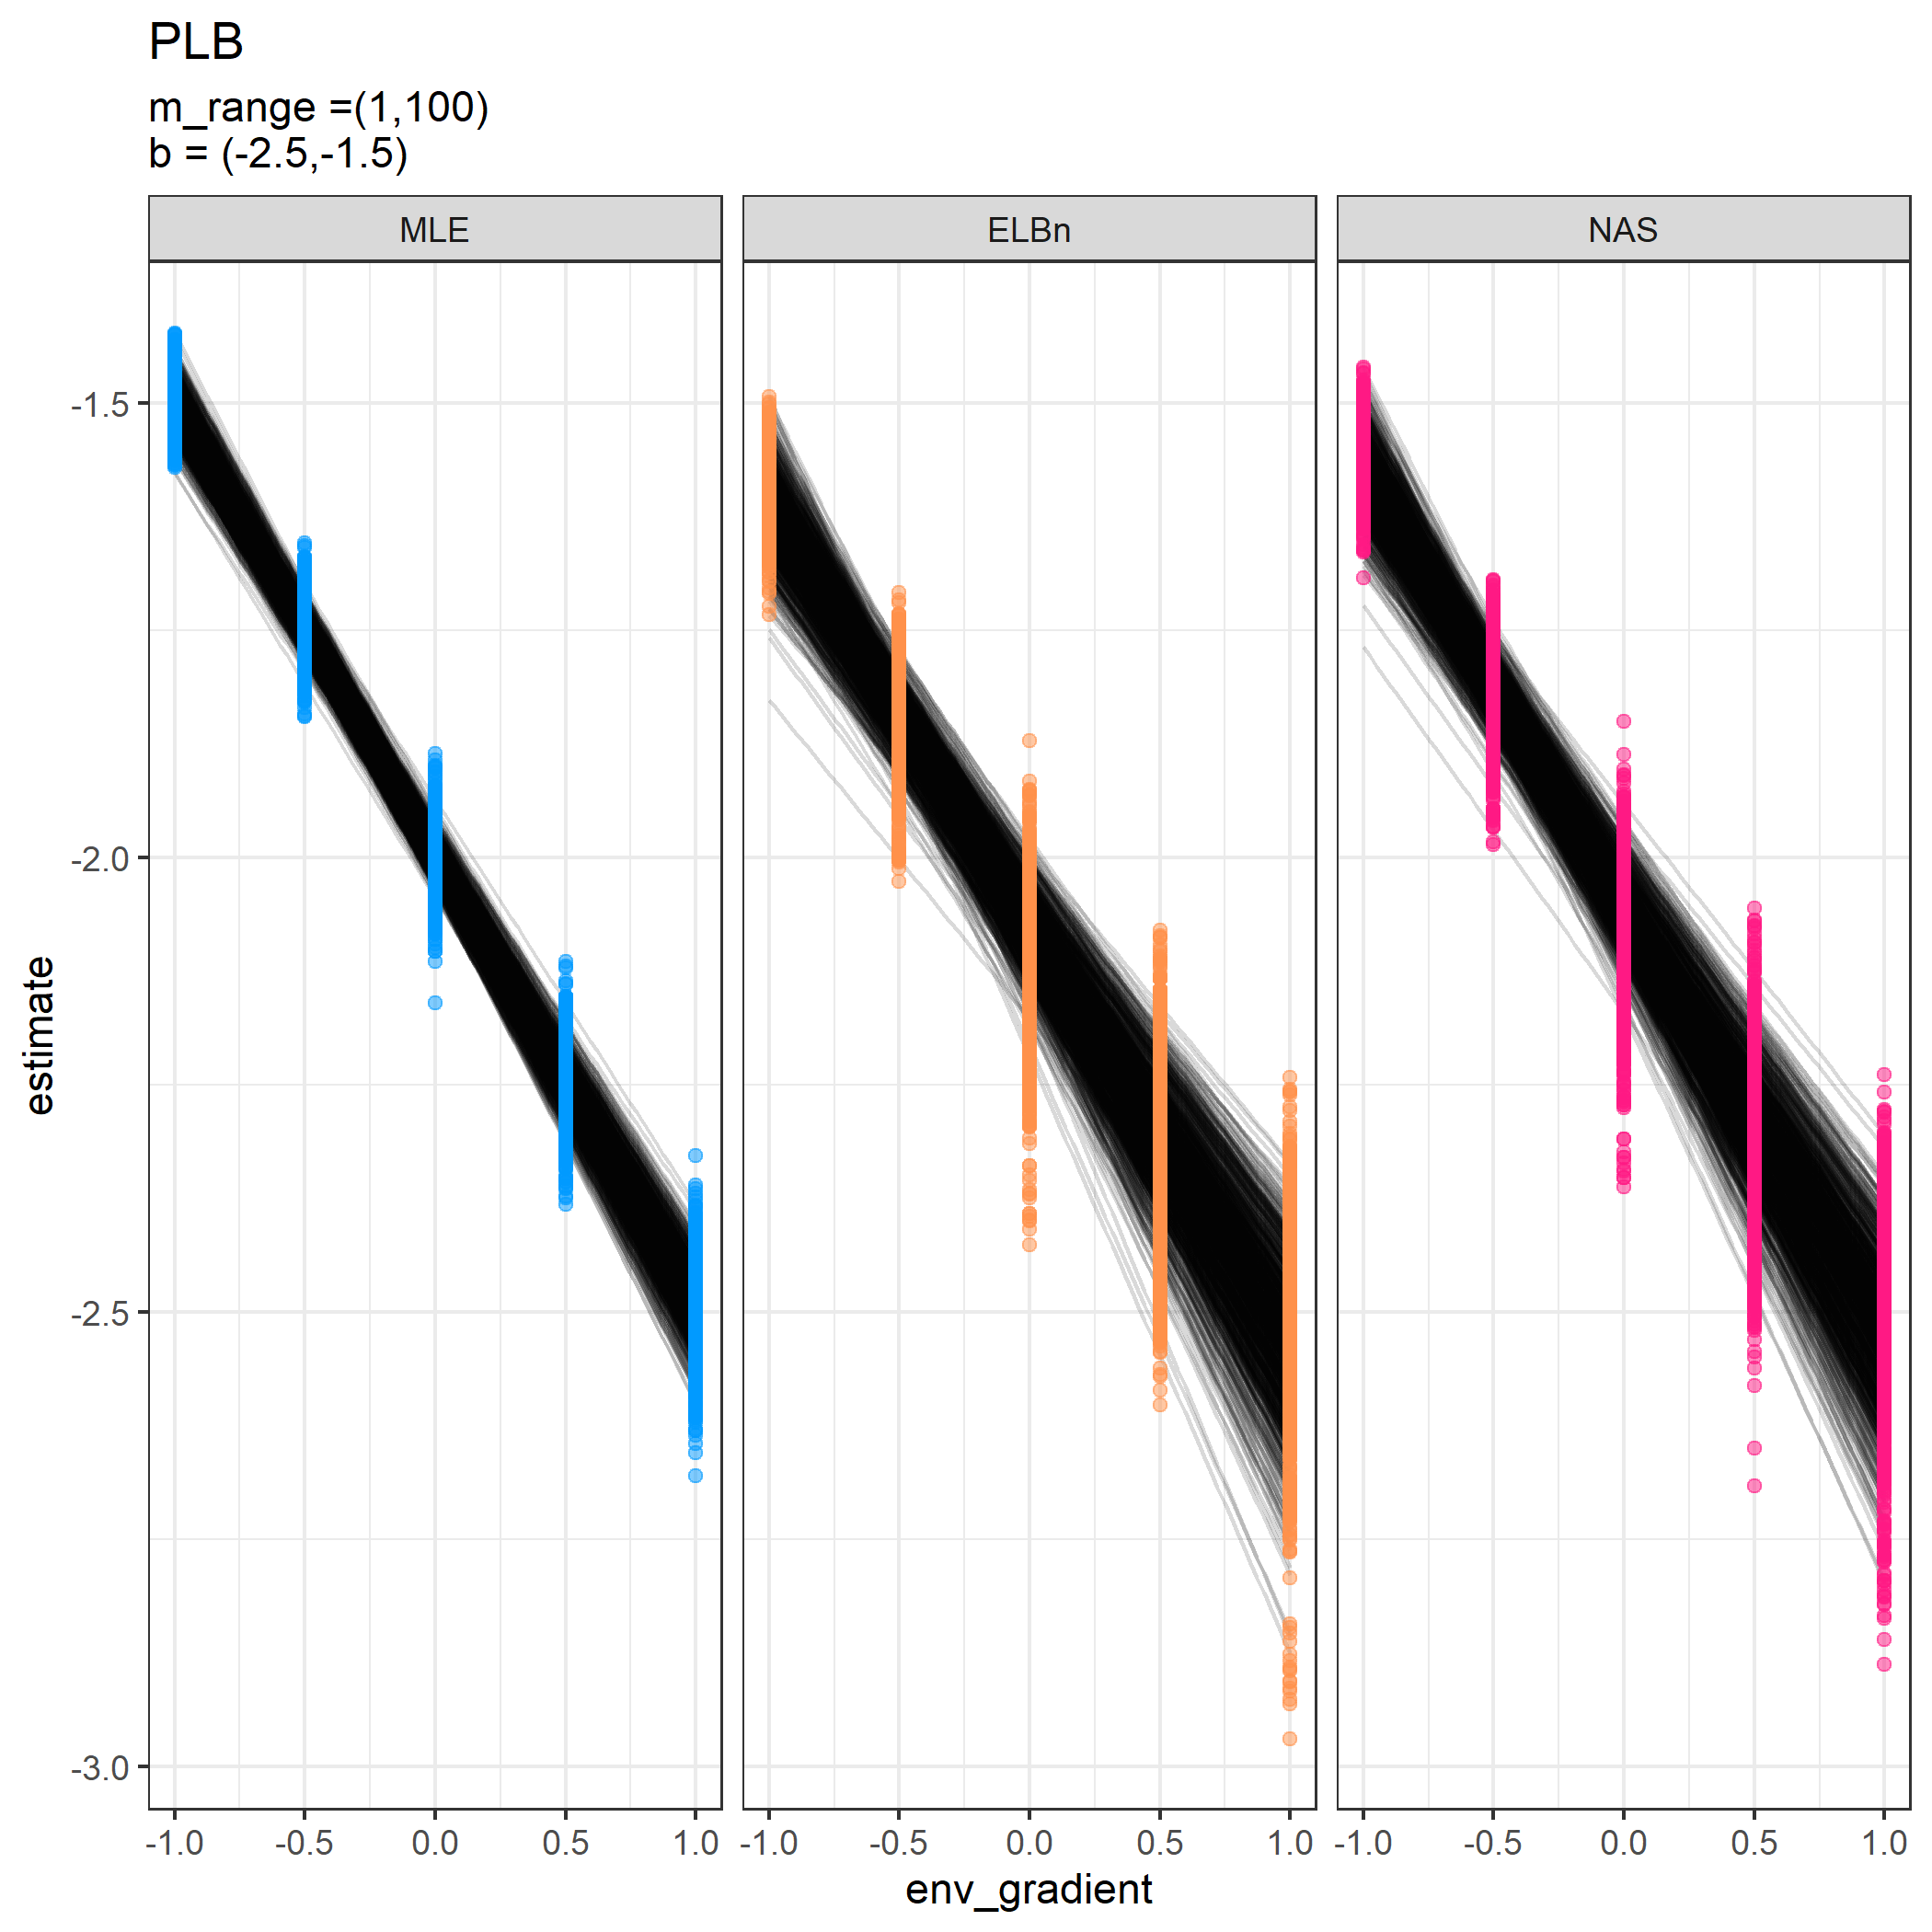
\includegraphics{figures/PLB_small_m_main.png}
\caption{Individual regressions for five sites across a hypothetical
gradient with a known relationship of 0.5. Range of body sizes is
reduced and is from 1, to 100.}
\end{figure}

\newpage

\begin{figure}
\centering
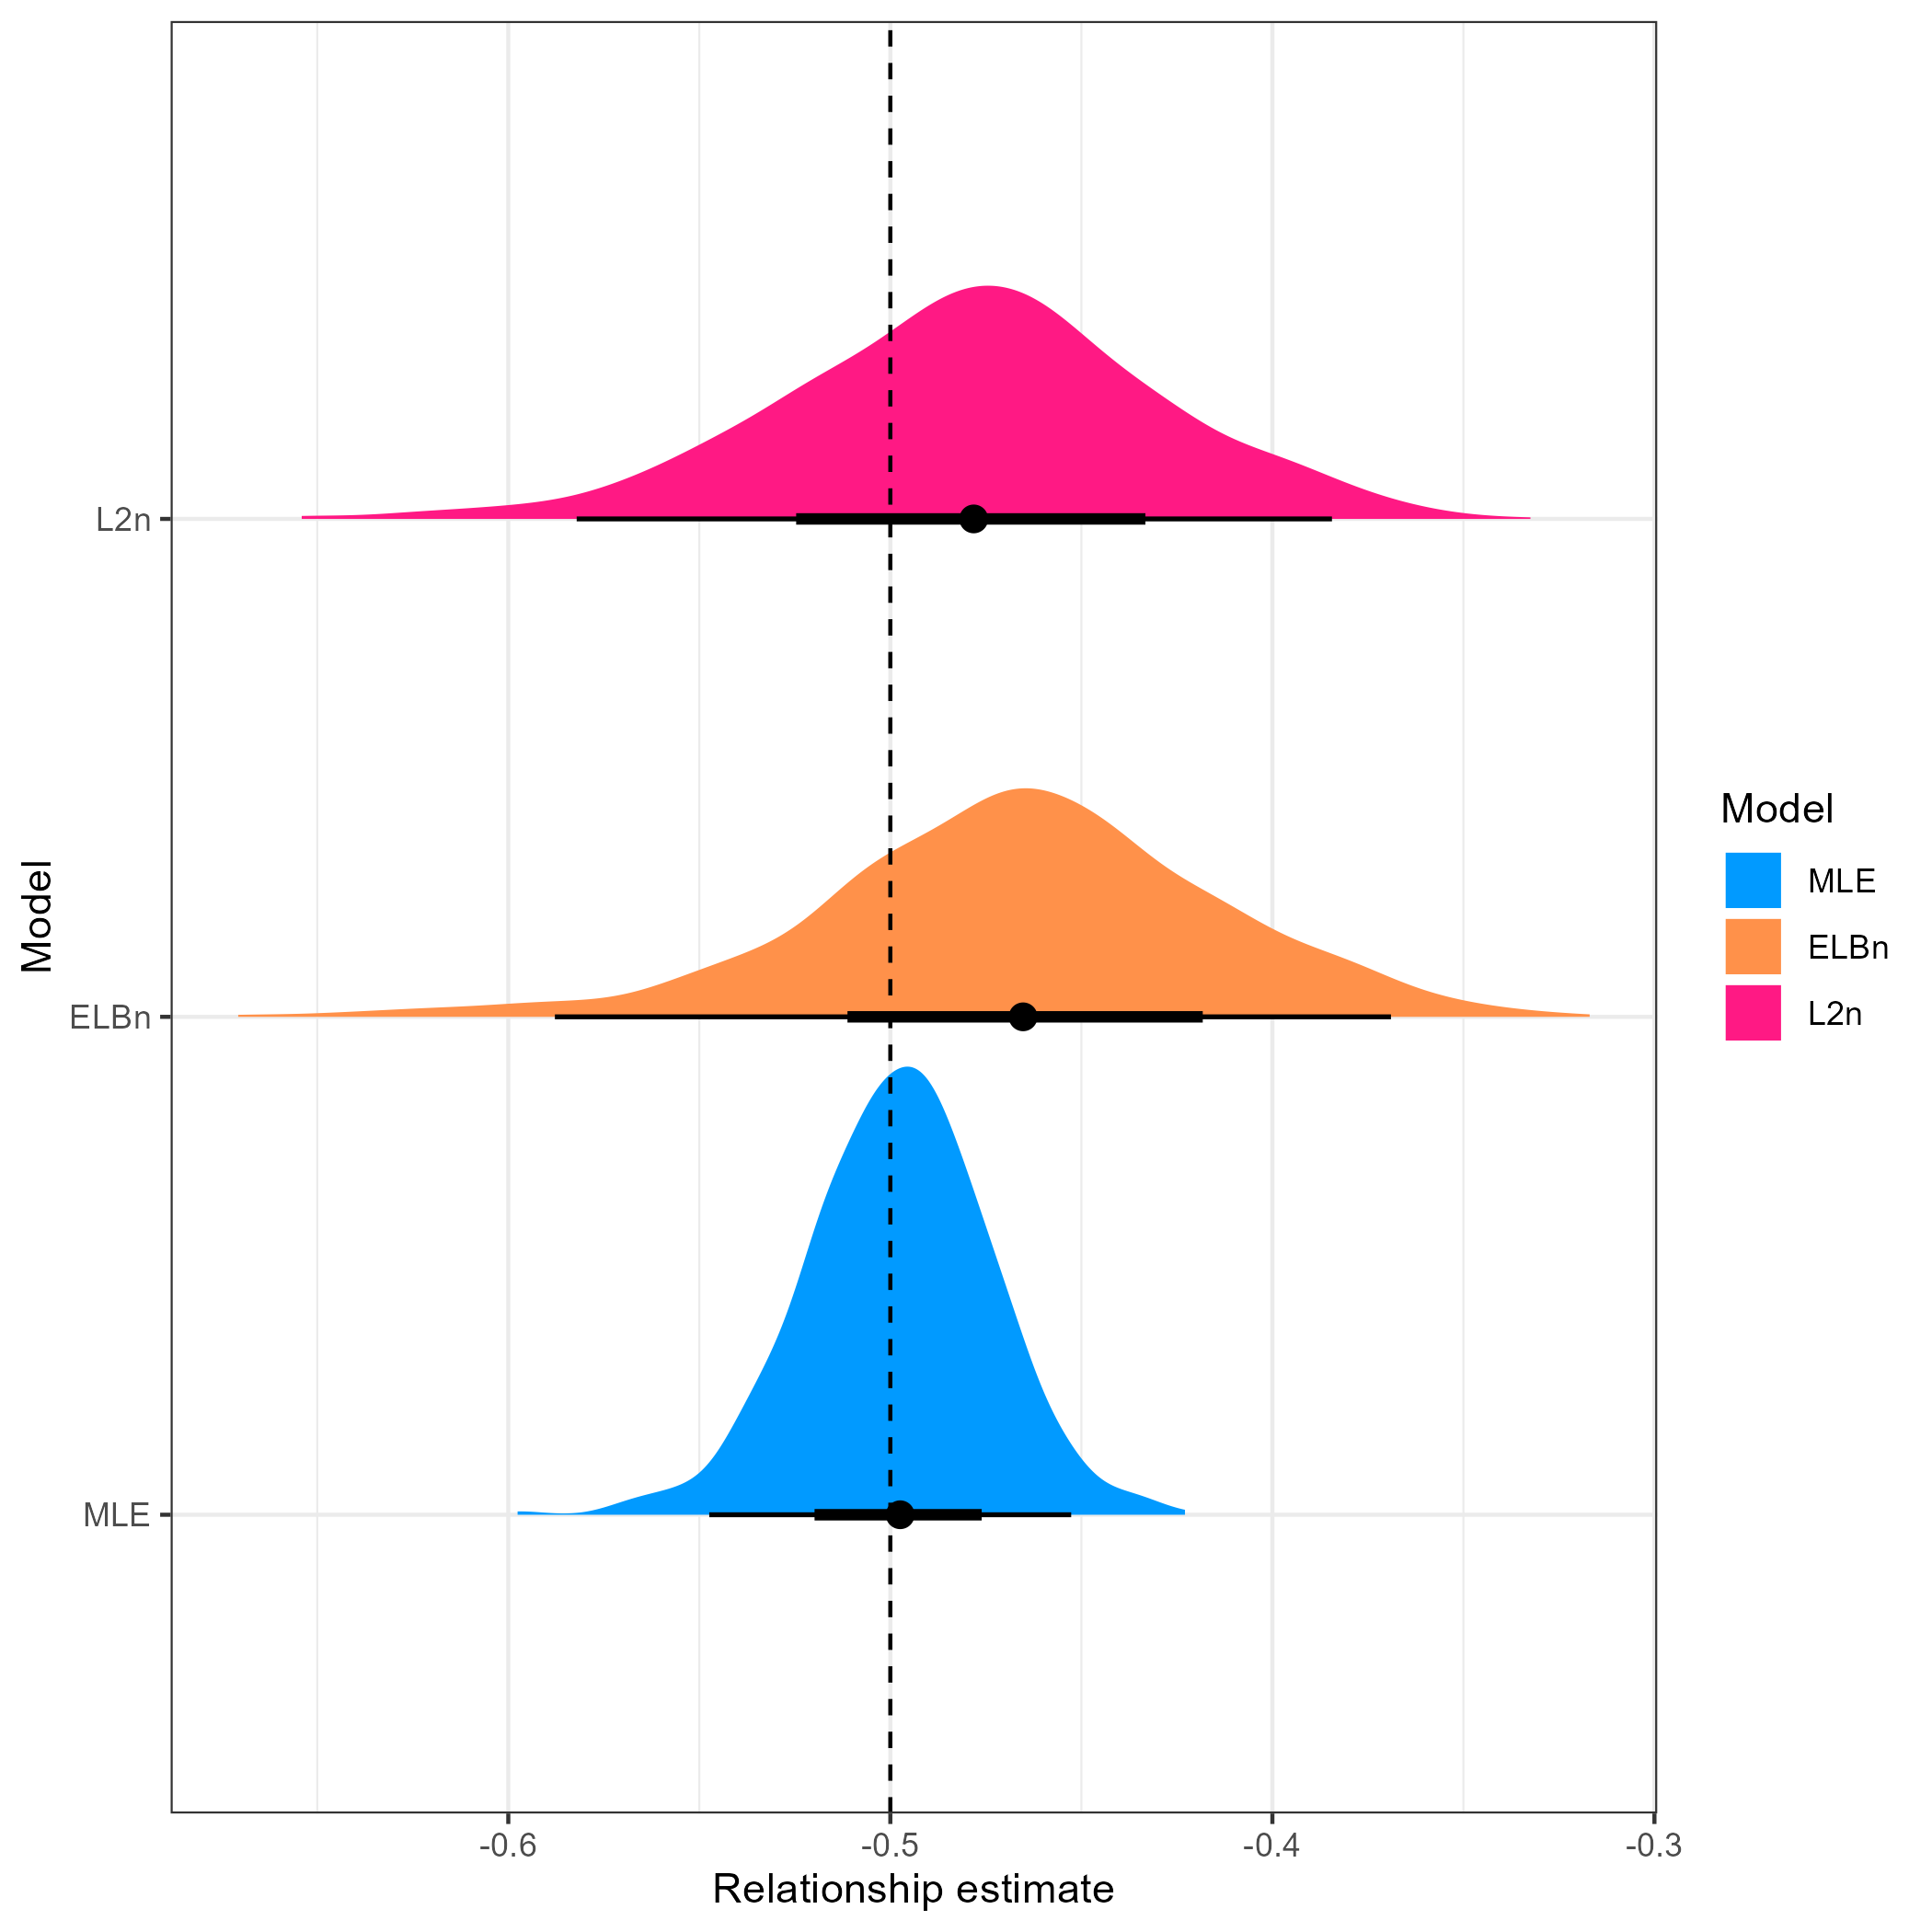
\includegraphics{figures/PLB_small_m_relationship_density.png}
\caption{Distribution of estimated relationship (\(\beta_1\))
coefficient's for five sites across a hypothetical gradient with known
value of 0.5. Range of body sizes is reduced and is from 1, to 100.}
\end{figure}

\newpage

\hypertarget{large-environmental-gradient}{%
\subsection{Large environmental
gradient}\label{large-environmental-gradient}}

\begin{figure}
\centering
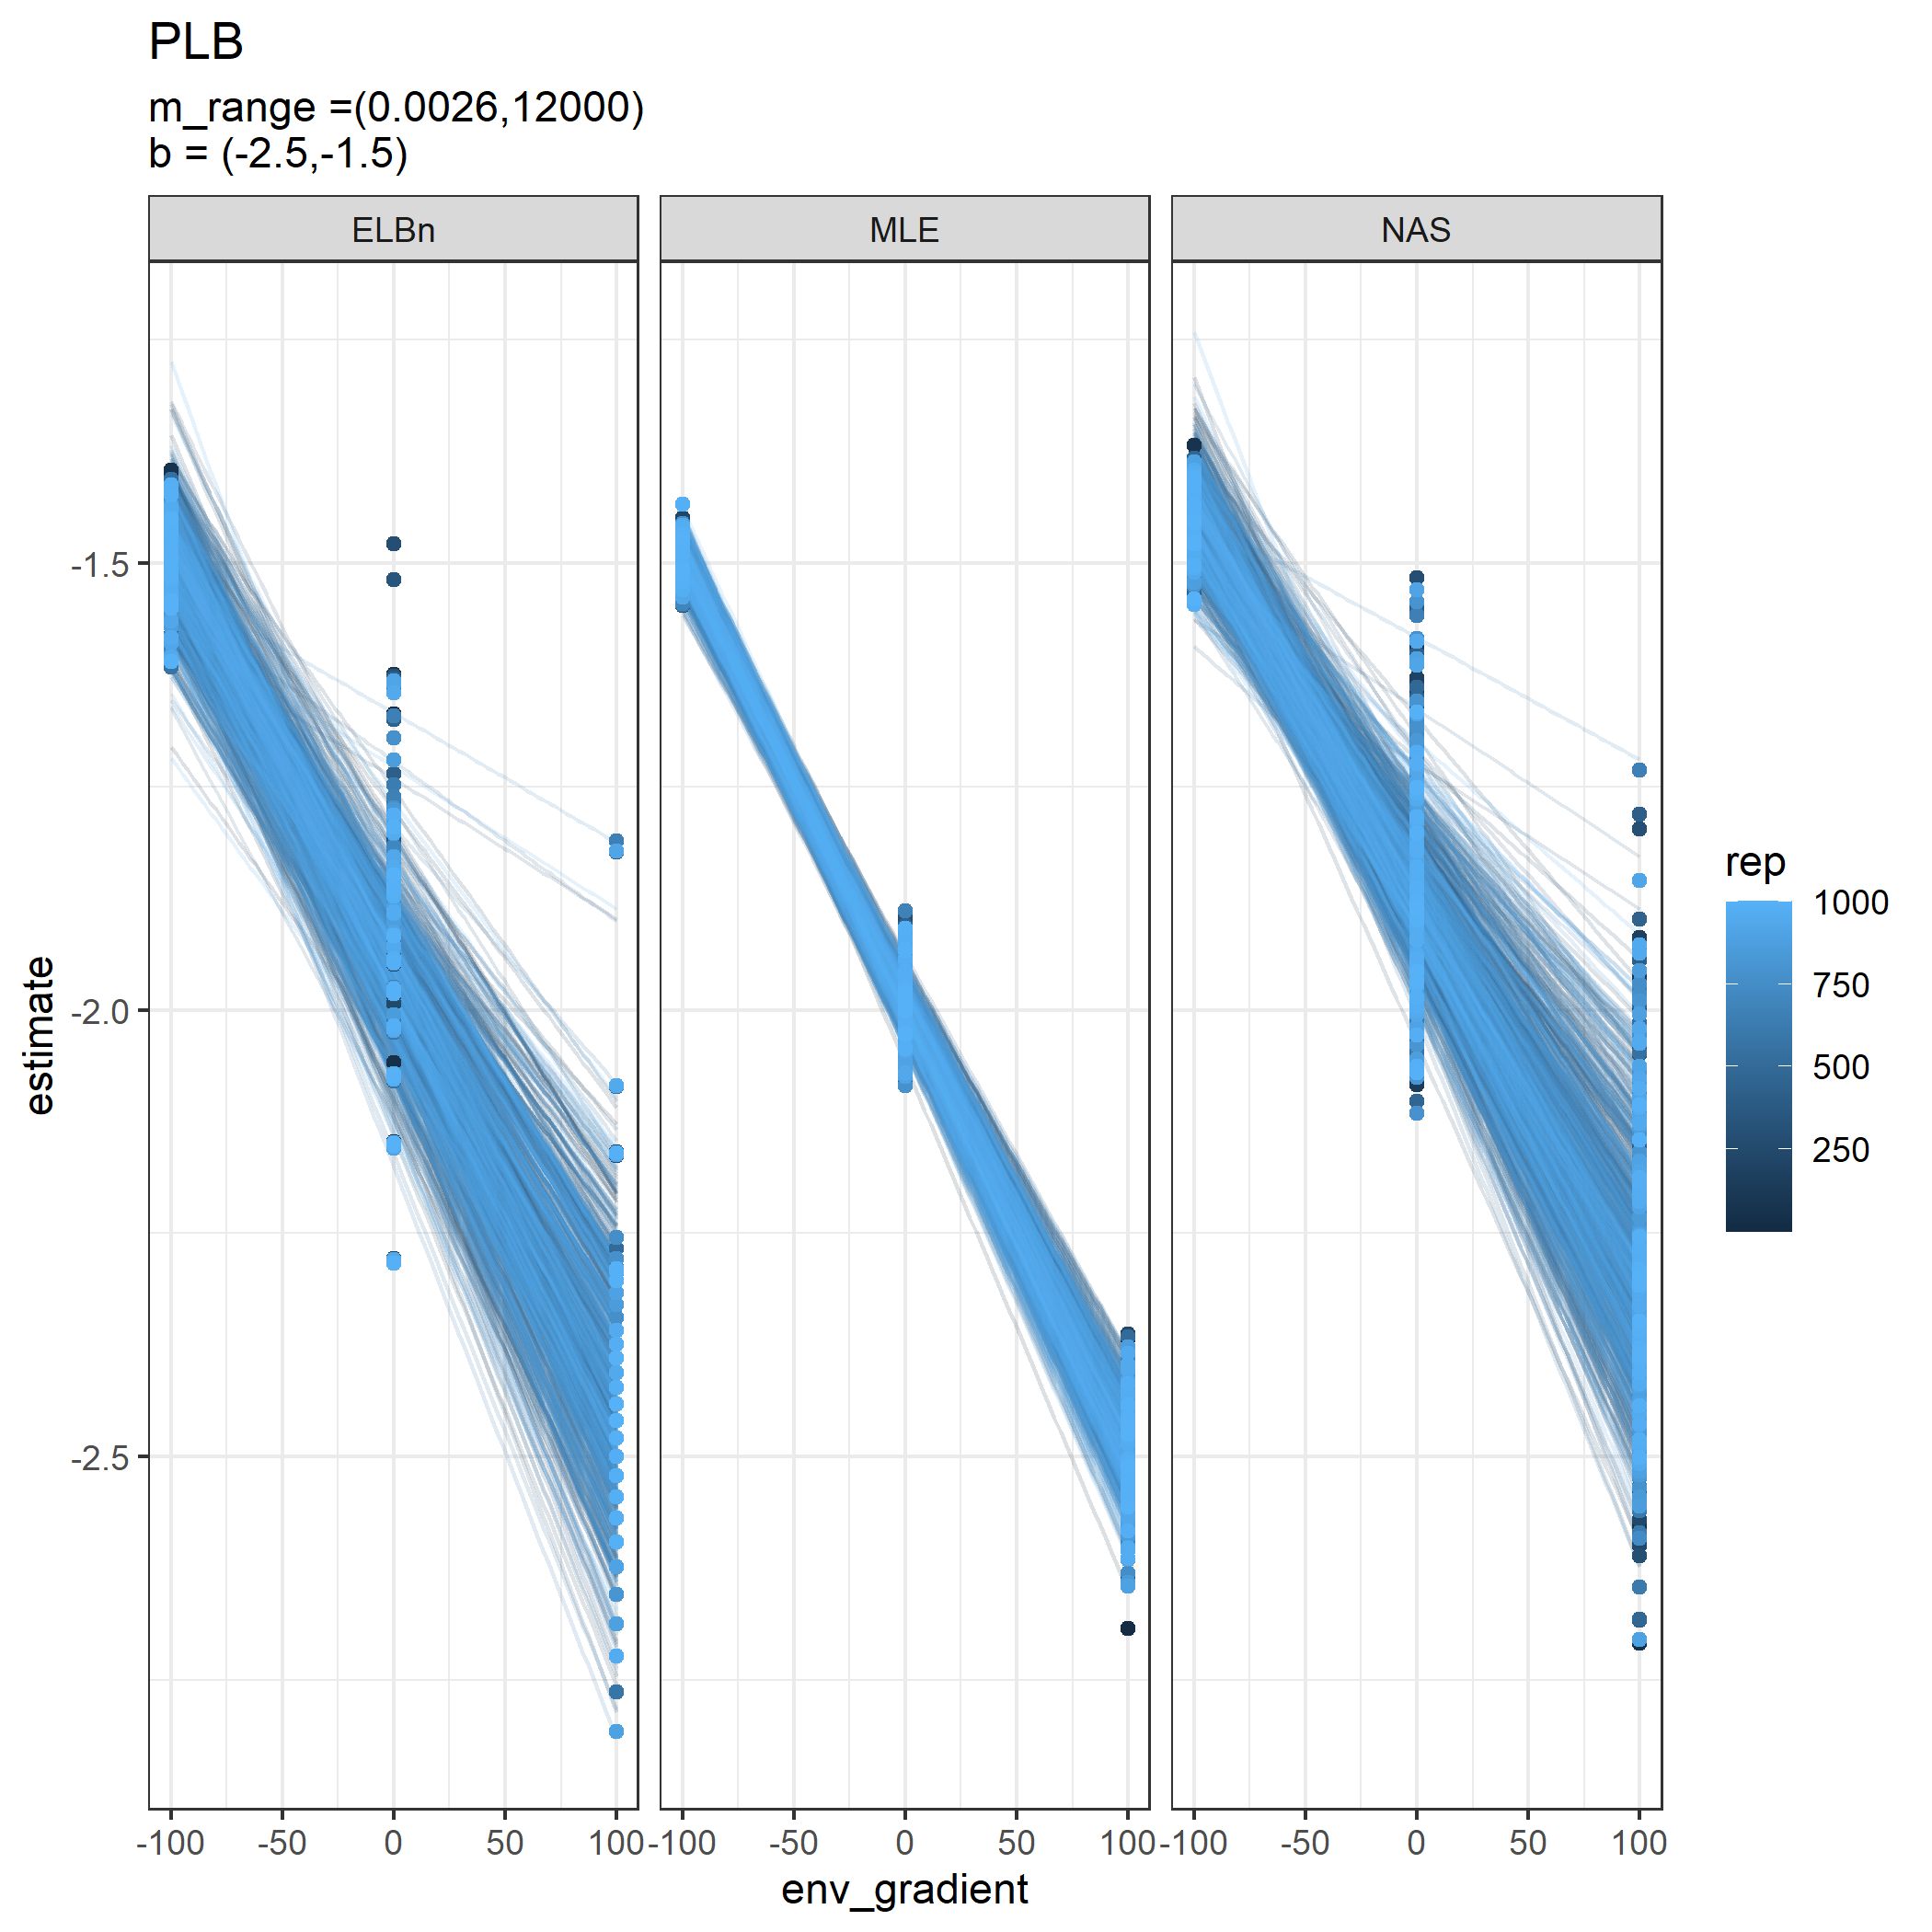
\includegraphics{figures/PLB_large_x_main.png}
\caption{Individual regressions for five sites across a hypothetical
gradient with a known relationship of 0.5. Range of environmental values
(\emph{x}-axis) increased to be -1000, to 1000.}
\end{figure}

\newpage

\begin{figure}
\centering
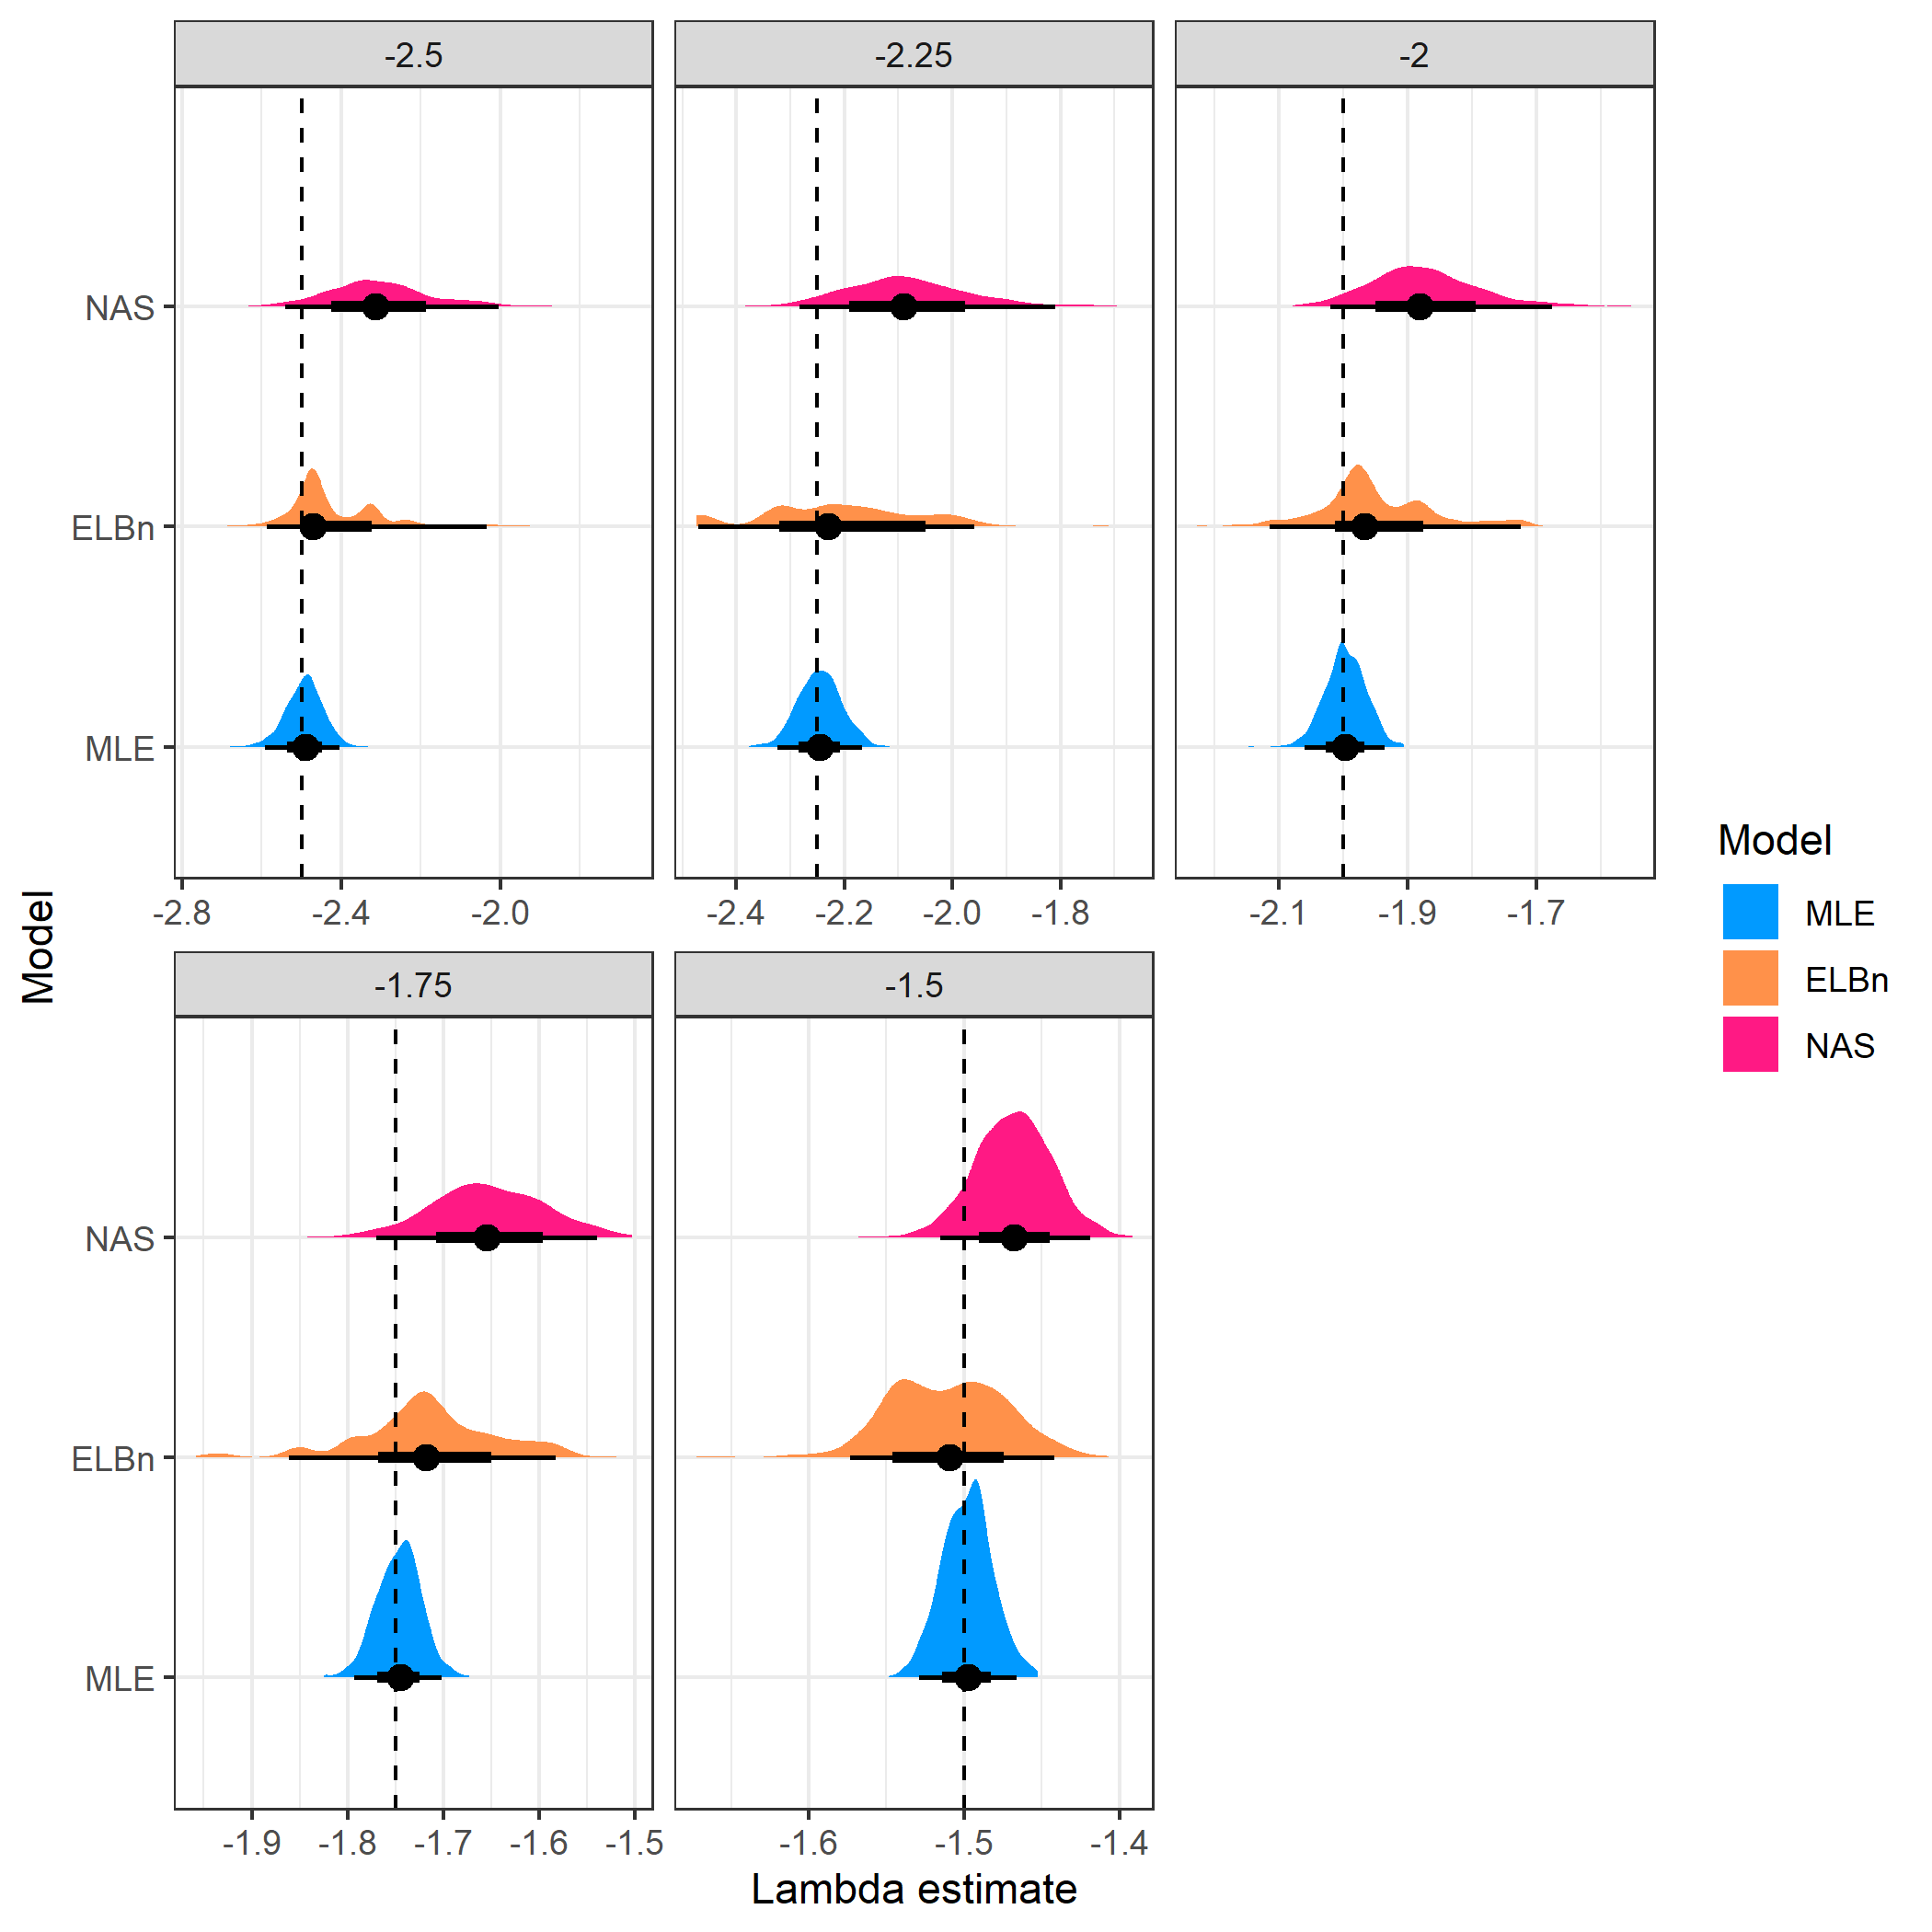
\includegraphics{figures/PLB_large_x_est_b_density.png}
\caption{Distribution of estimated \(\lambda\) coefficient for five
sites across a hypothetical gradient with known values. Range of
environmental values (\emph{x}-axis) increased to be -1000, to 1000.}
\end{figure}

\newpage

\begin{figure}
\centering
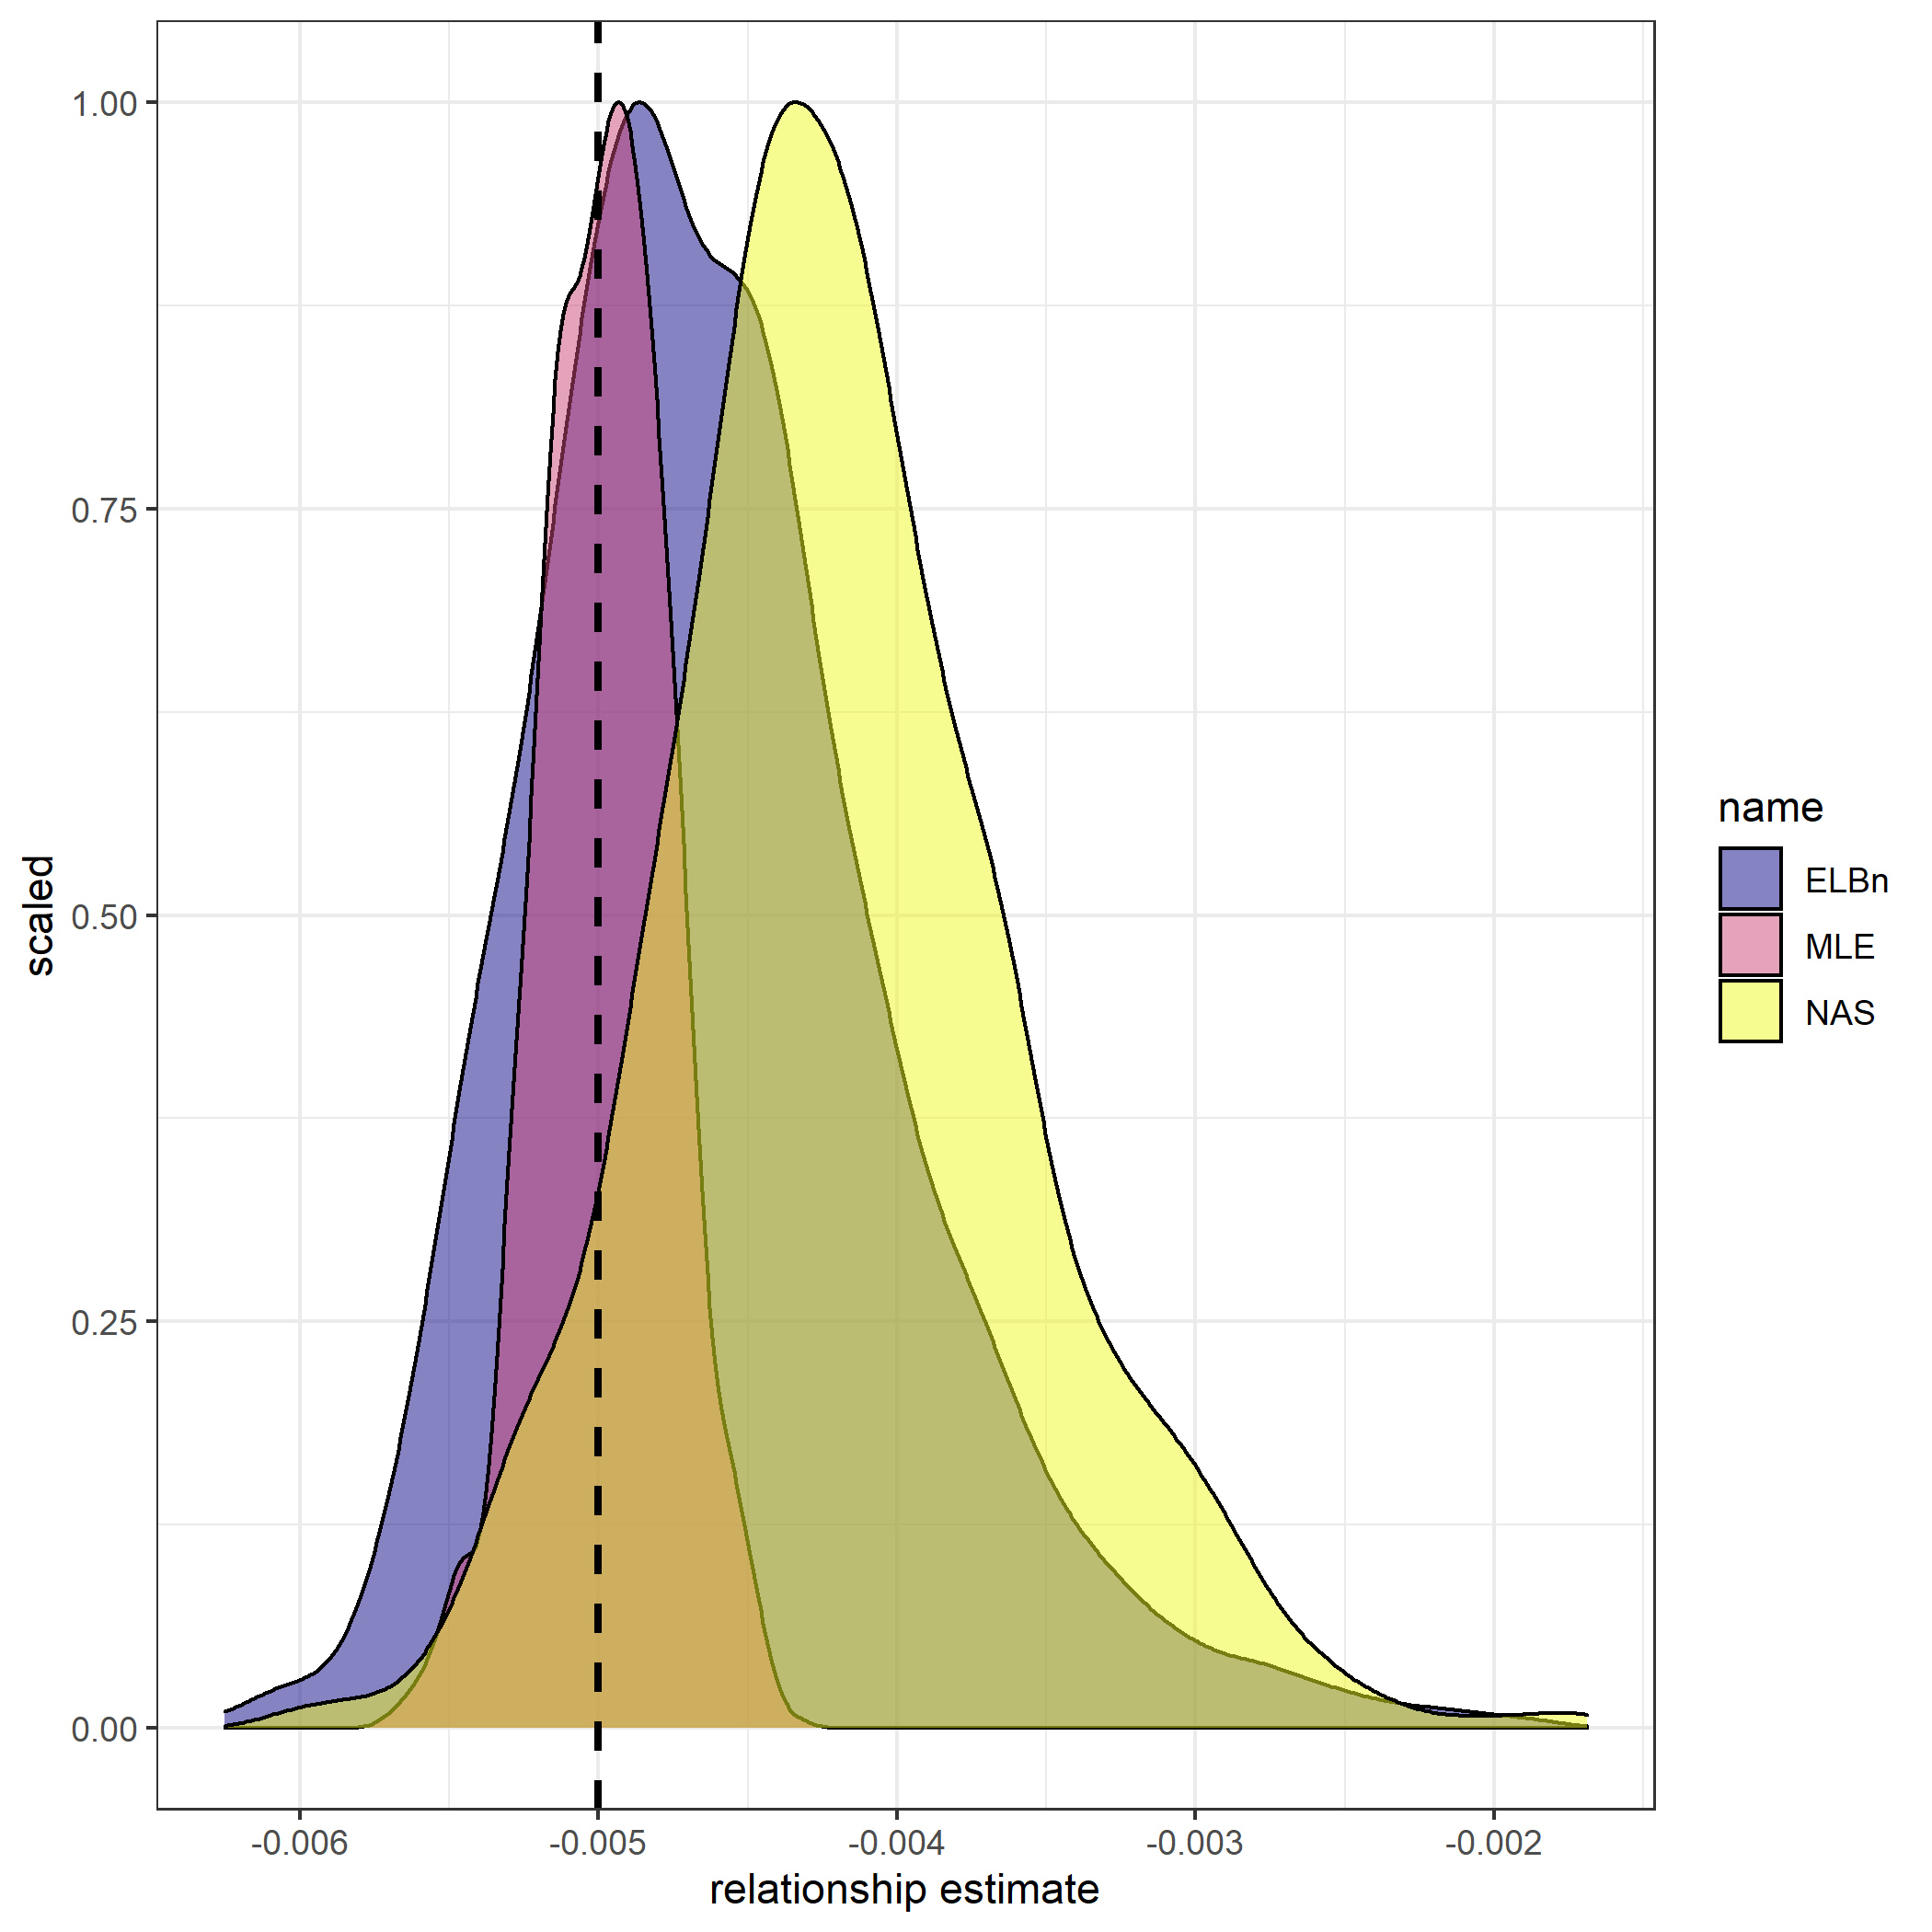
\includegraphics{figures/PLB_large_x_relationship_density.png}
\caption{Distribution of estimated relationship (\(\beta_1\))
coefficient's for five sites across a hypothetical gradient with known
value of 0.5. Range of environmental values (\emph{x}-axis) increased to
be -1000, to 1000.}
\end{figure}

\newpage

\hypertarget{varying-number-of-sites}{%
\subsection{Varying number of sites}\label{varying-number-of-sites}}

\hypertarget{sites}{%
\subsubsection{10 sites}\label{sites}}

\begin{figure}
\centering
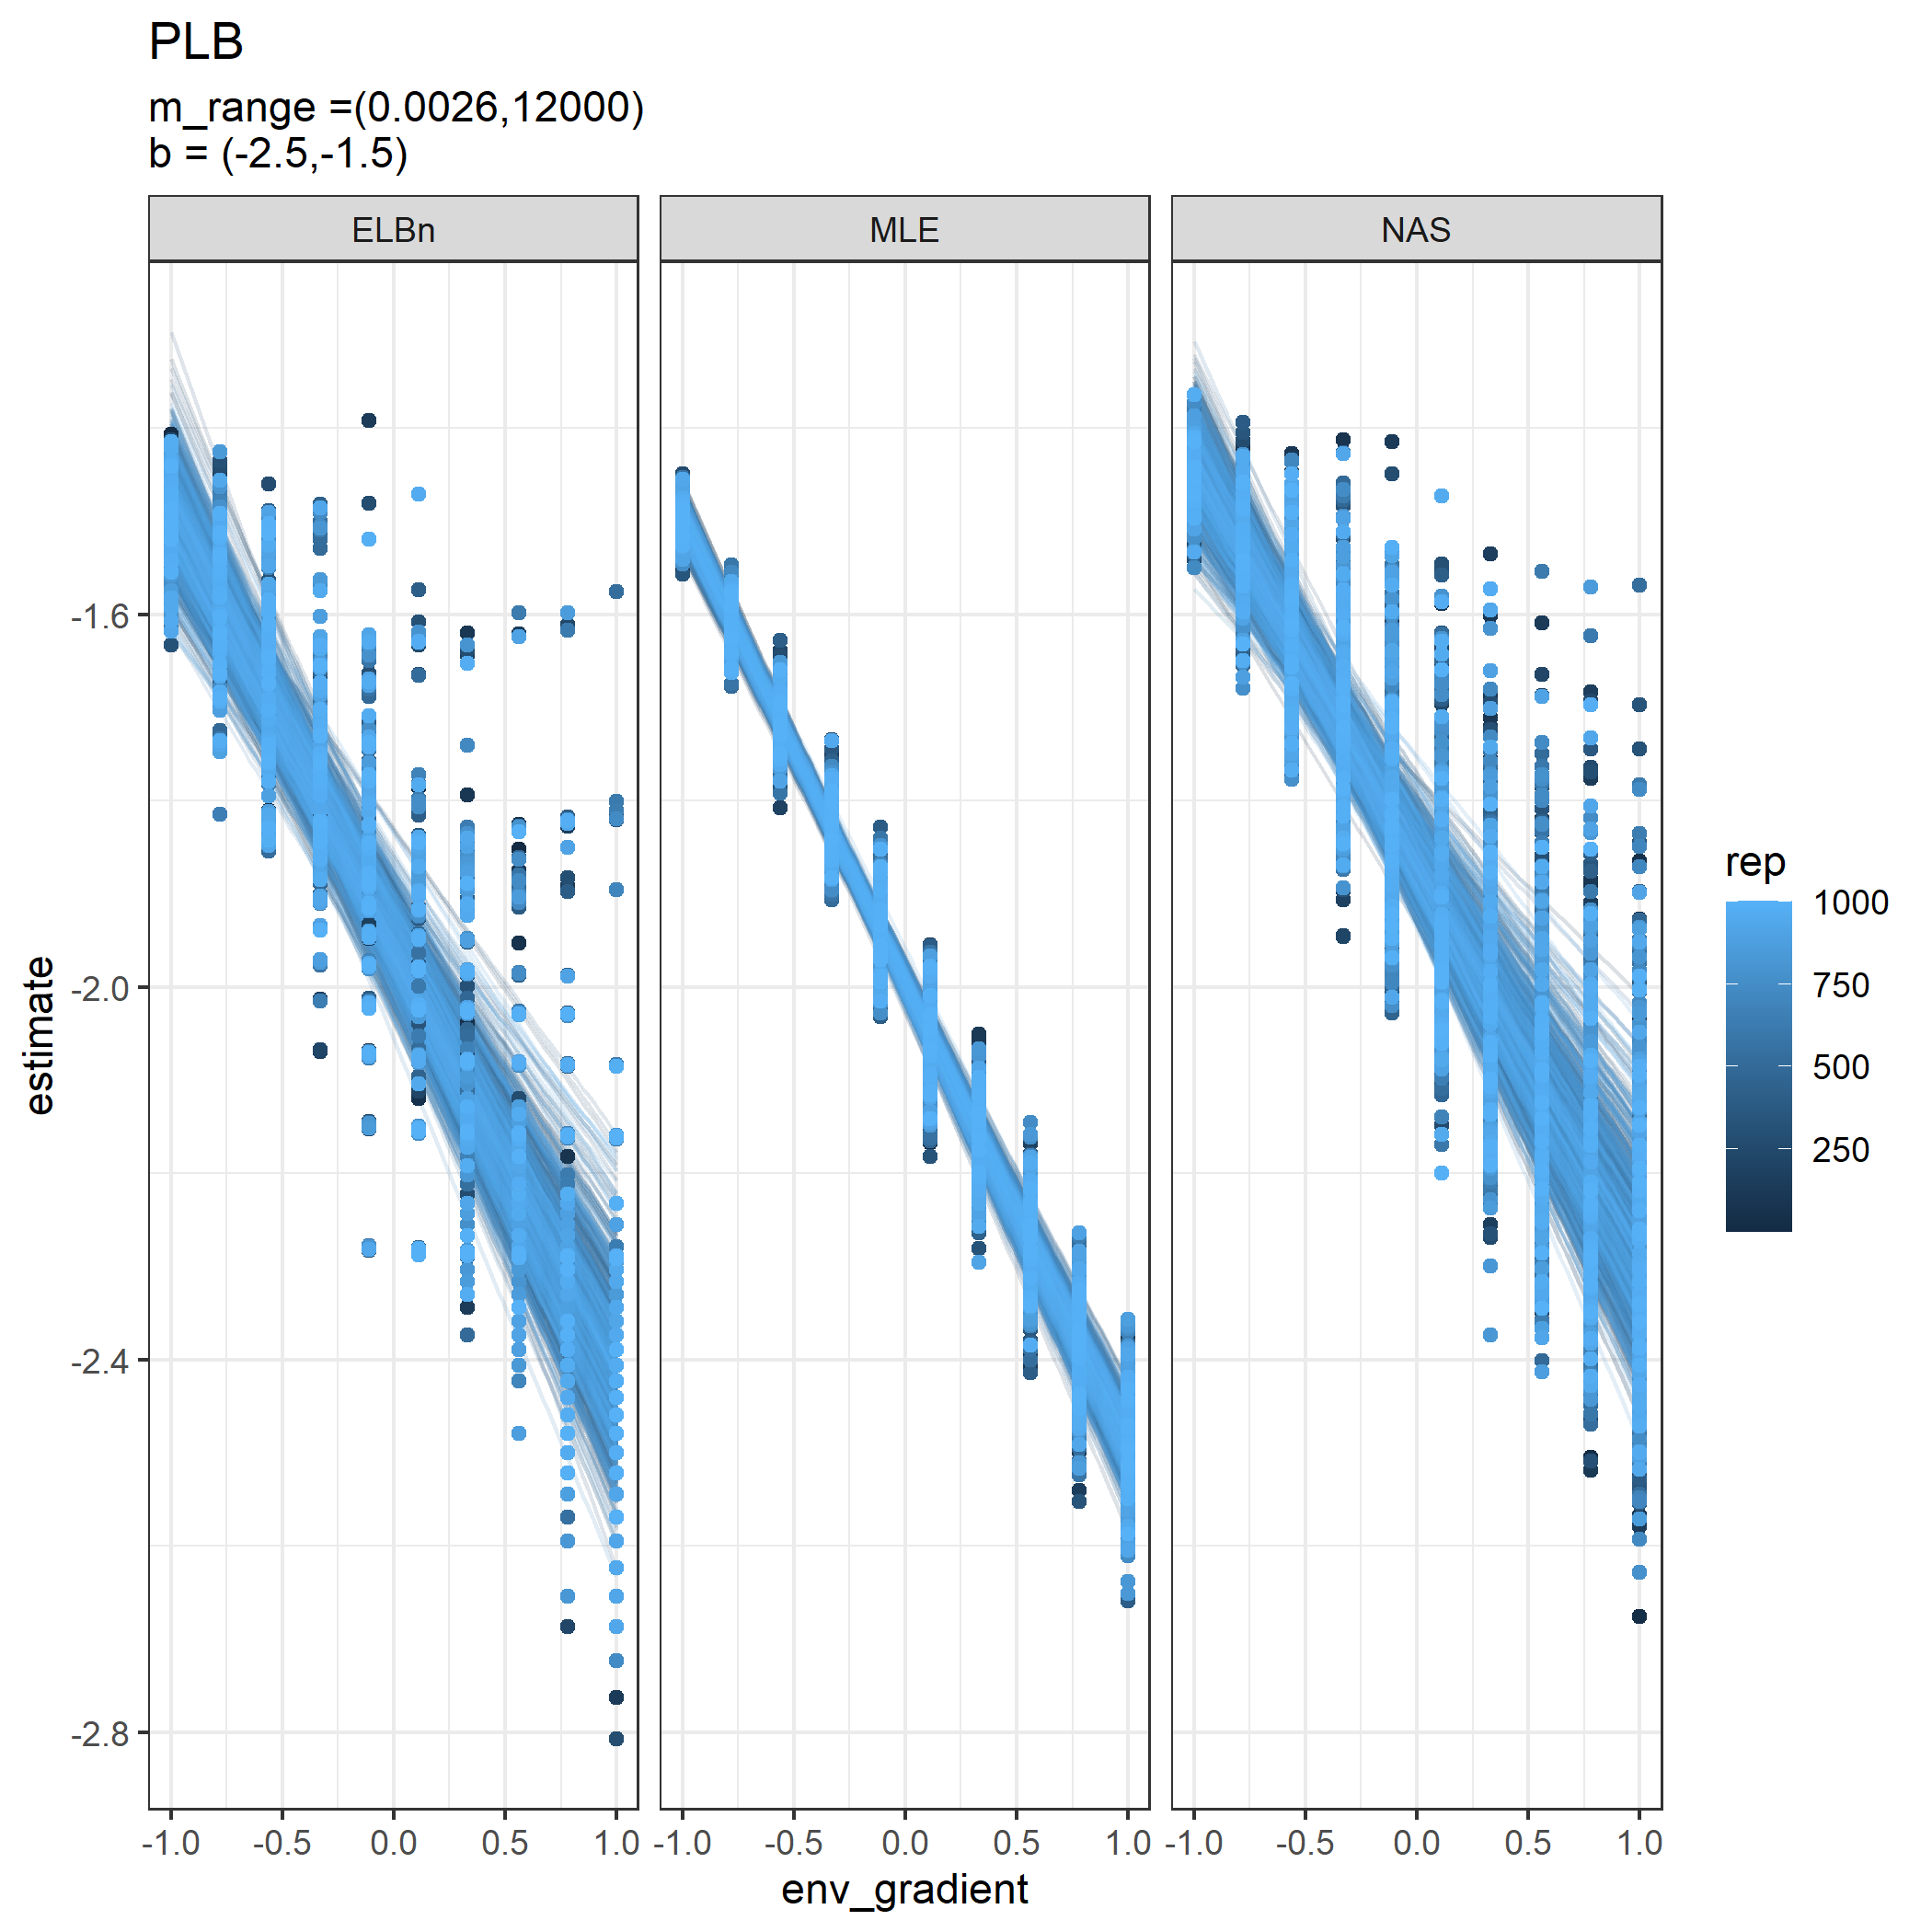
\includegraphics{figures/PLB_10_sites_main.png}
\caption{Individual regressions for ten sites across a hypothetical
gradient with a known relationship of 0.5. All other parameters are the
same as in the main analysis}
\end{figure}

\newpage

\begin{figure}
\centering
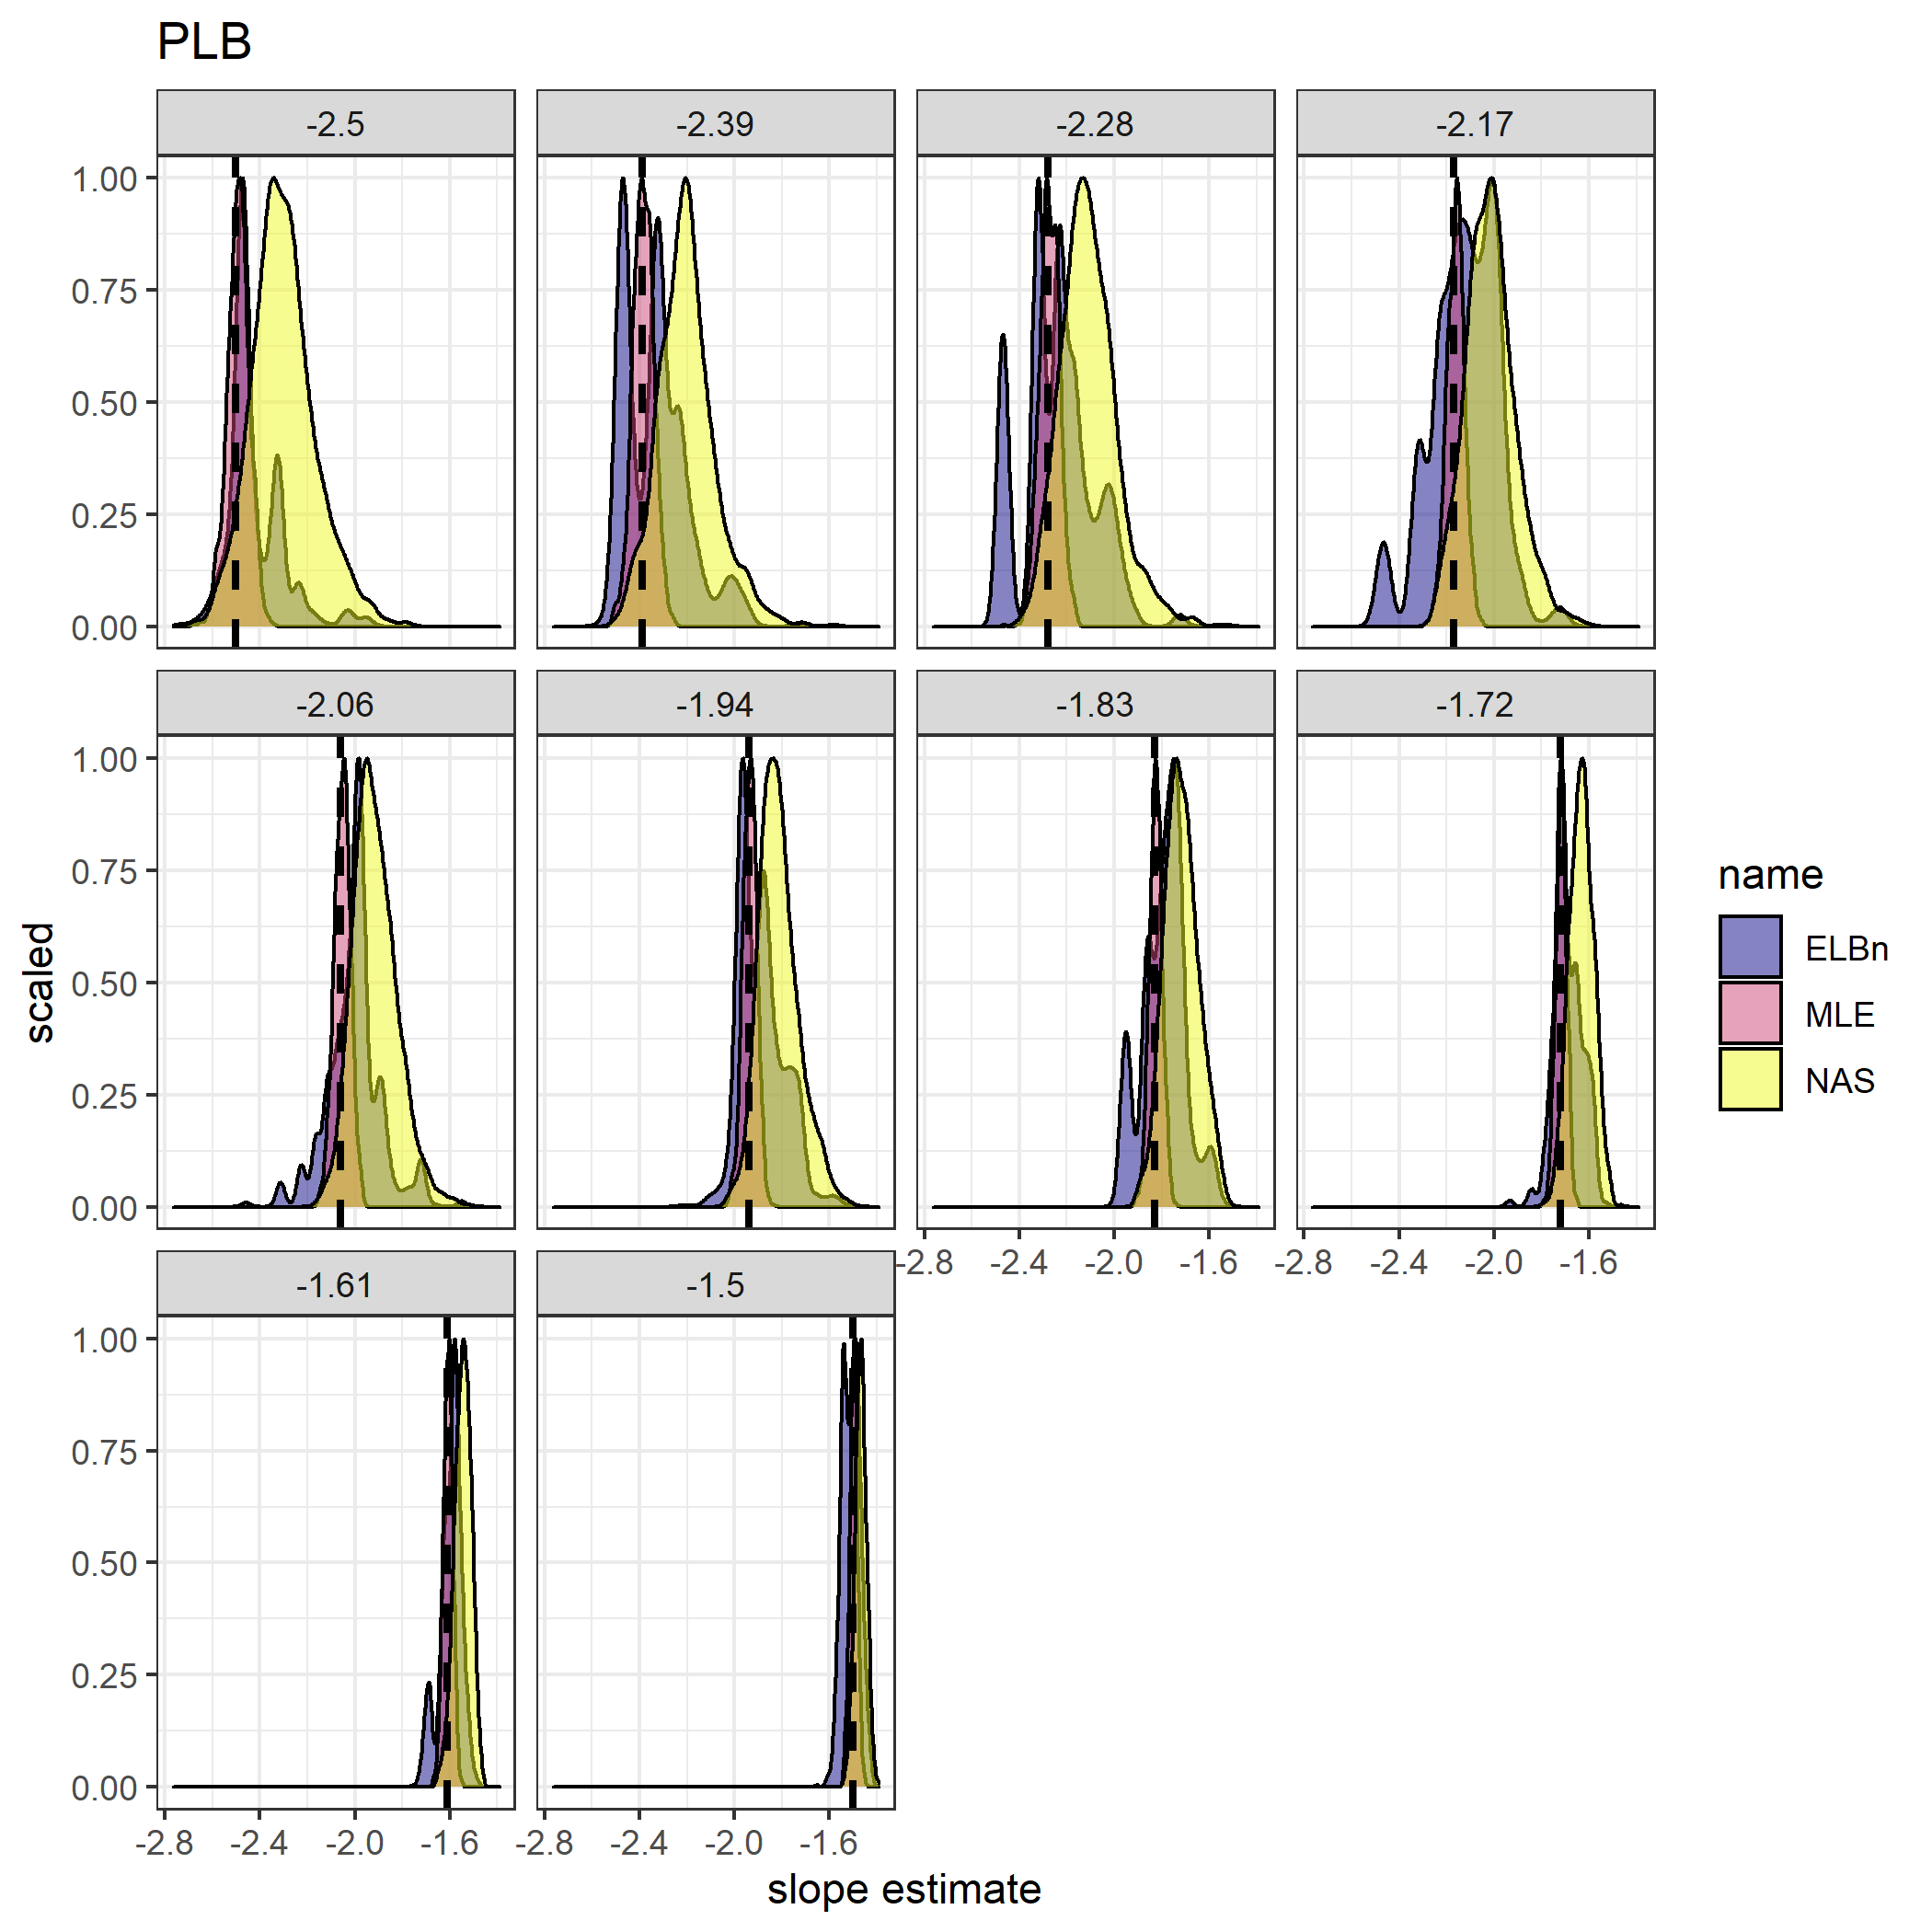
\includegraphics{figures/PLB_10_sites_est_b_density.png}
\caption{Distribution of estimated \(\lambda\) coefficient for ten sites
across a hypothetical gradient with known values. All other parameters
are the same as in the main analysis}
\end{figure}

\newpage

\begin{figure}
\centering
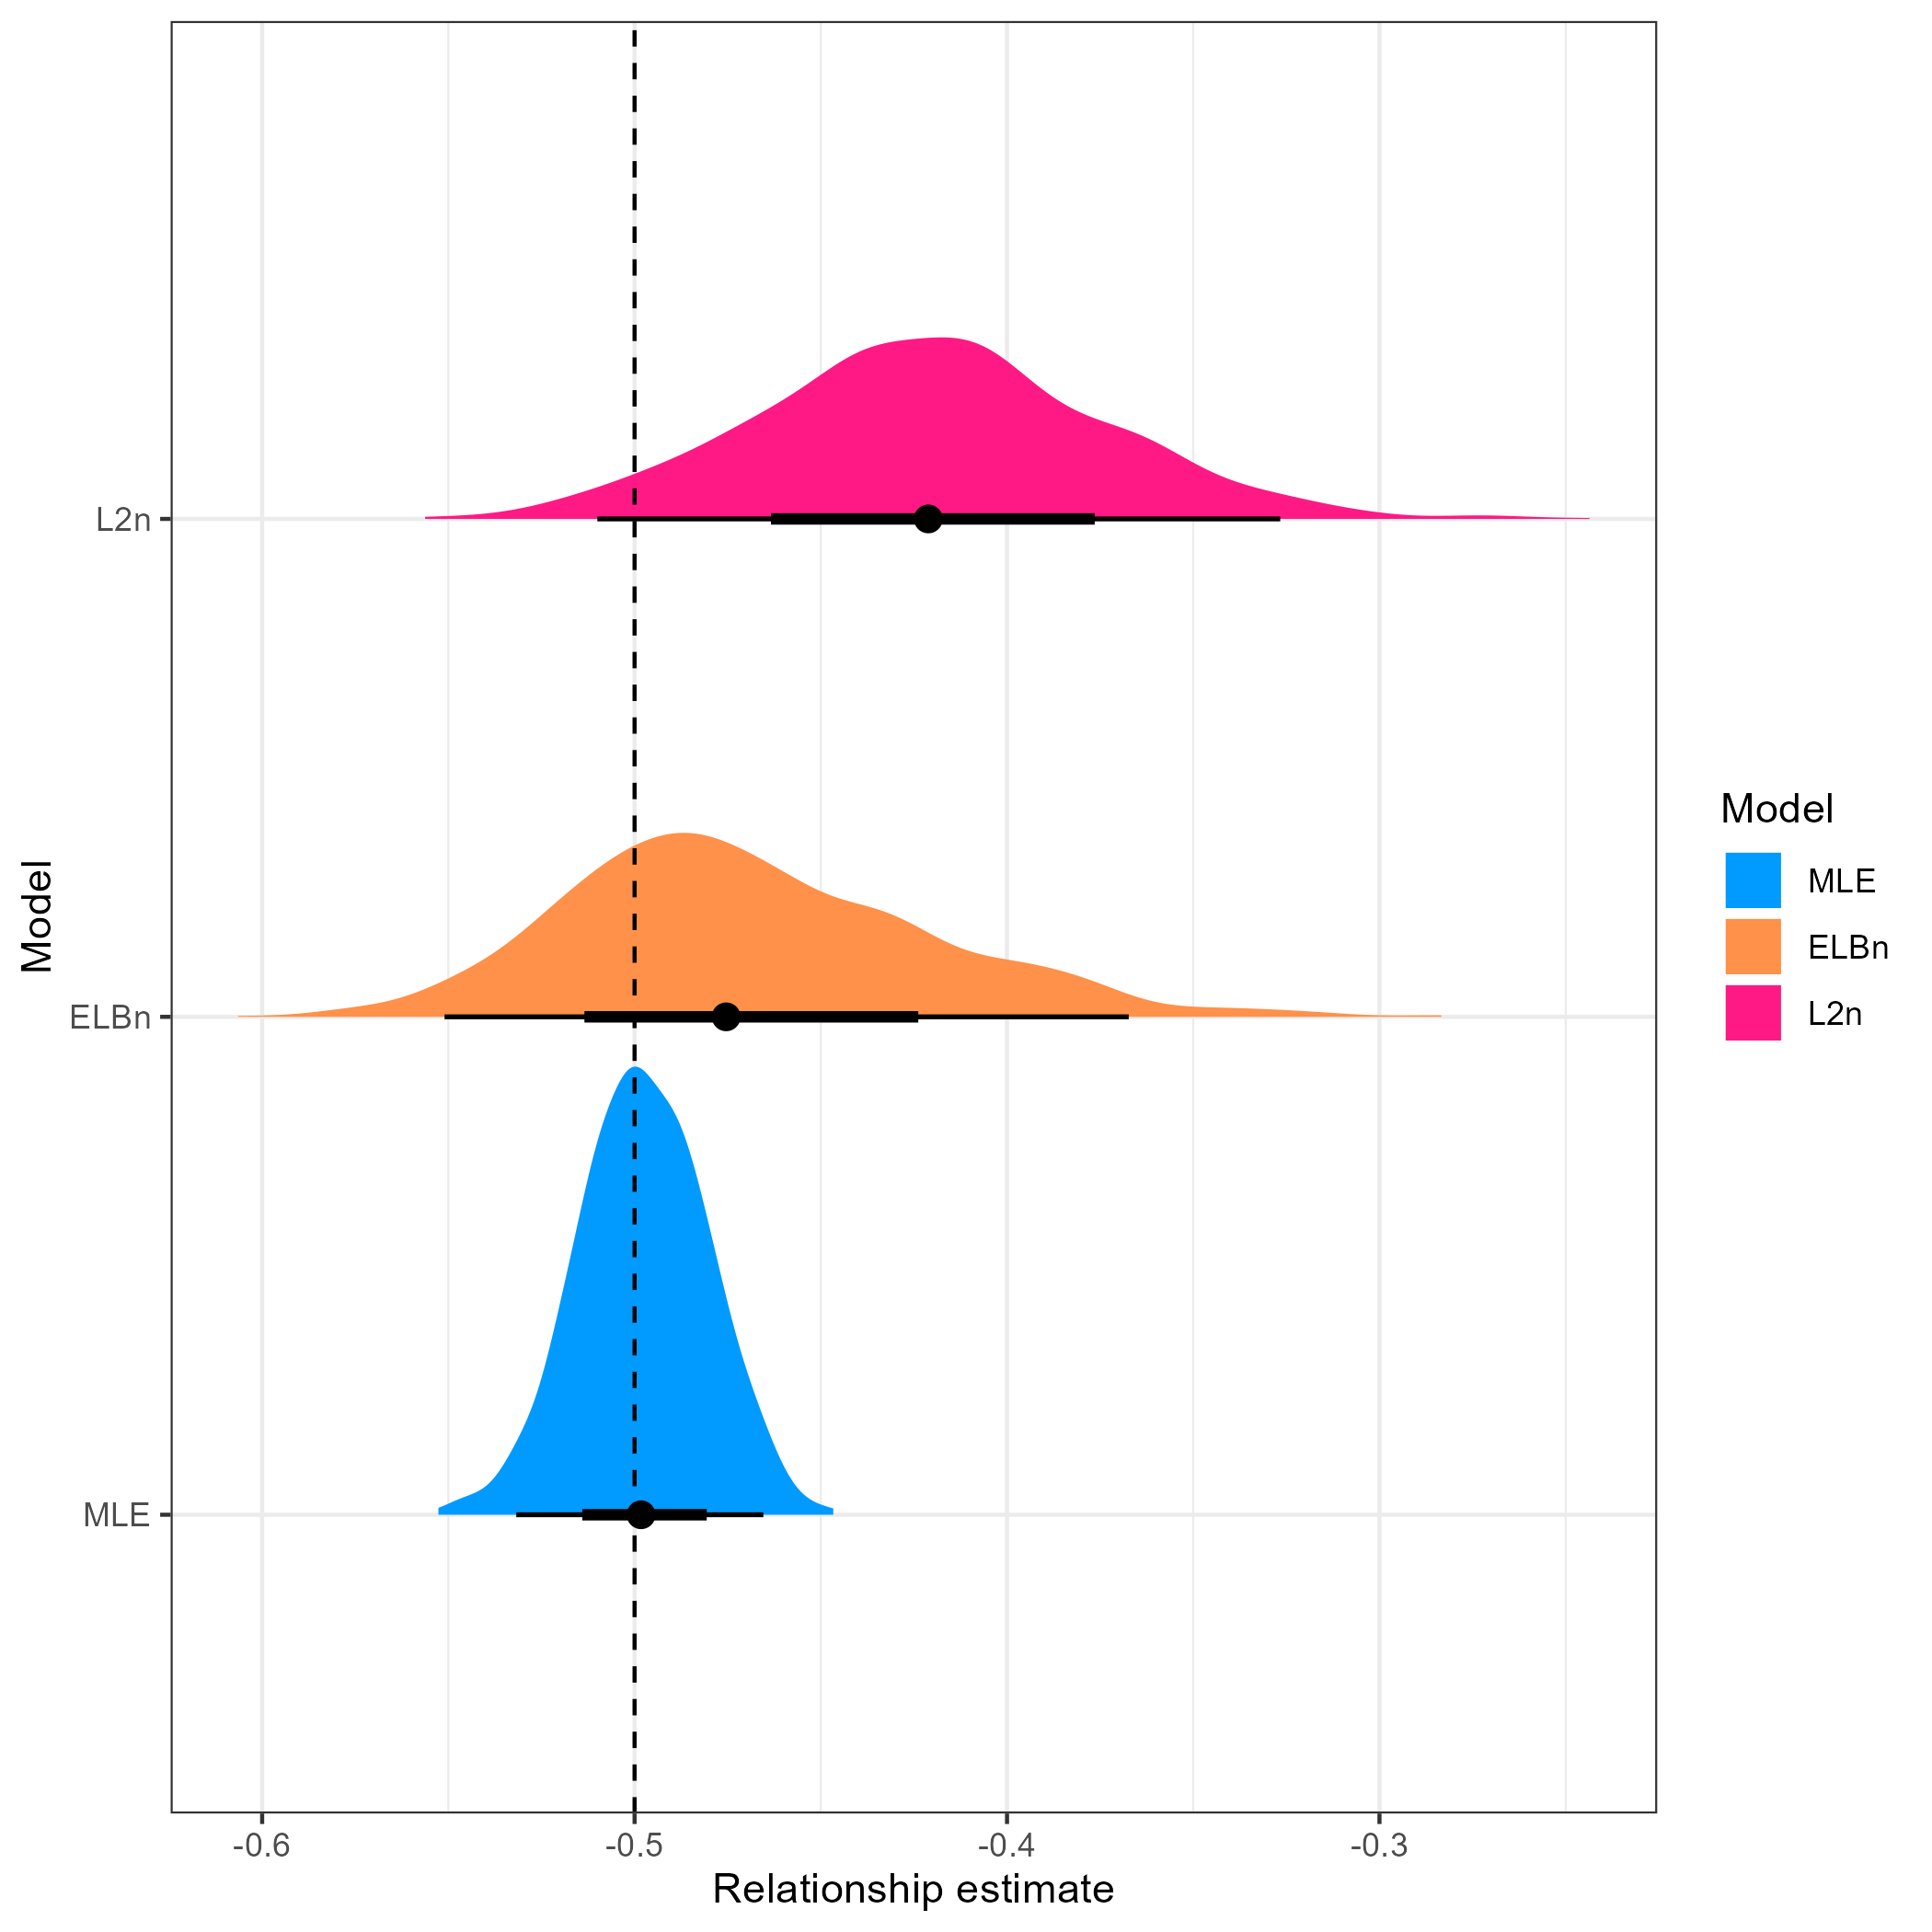
\includegraphics{figures/PLB_10_sites_relationship_density.png}
\caption{Distribution of estimated relationship (\(\beta_1\))
coefficient's for ten sites across a hypothetical gradient with known
value of 0.5. All other parameters are the same as in the main analysis}
\end{figure}

\newpage

\hypertarget{three-sites}{%
\subsubsection{Three sites}\label{three-sites}}

\begin{figure}
\centering
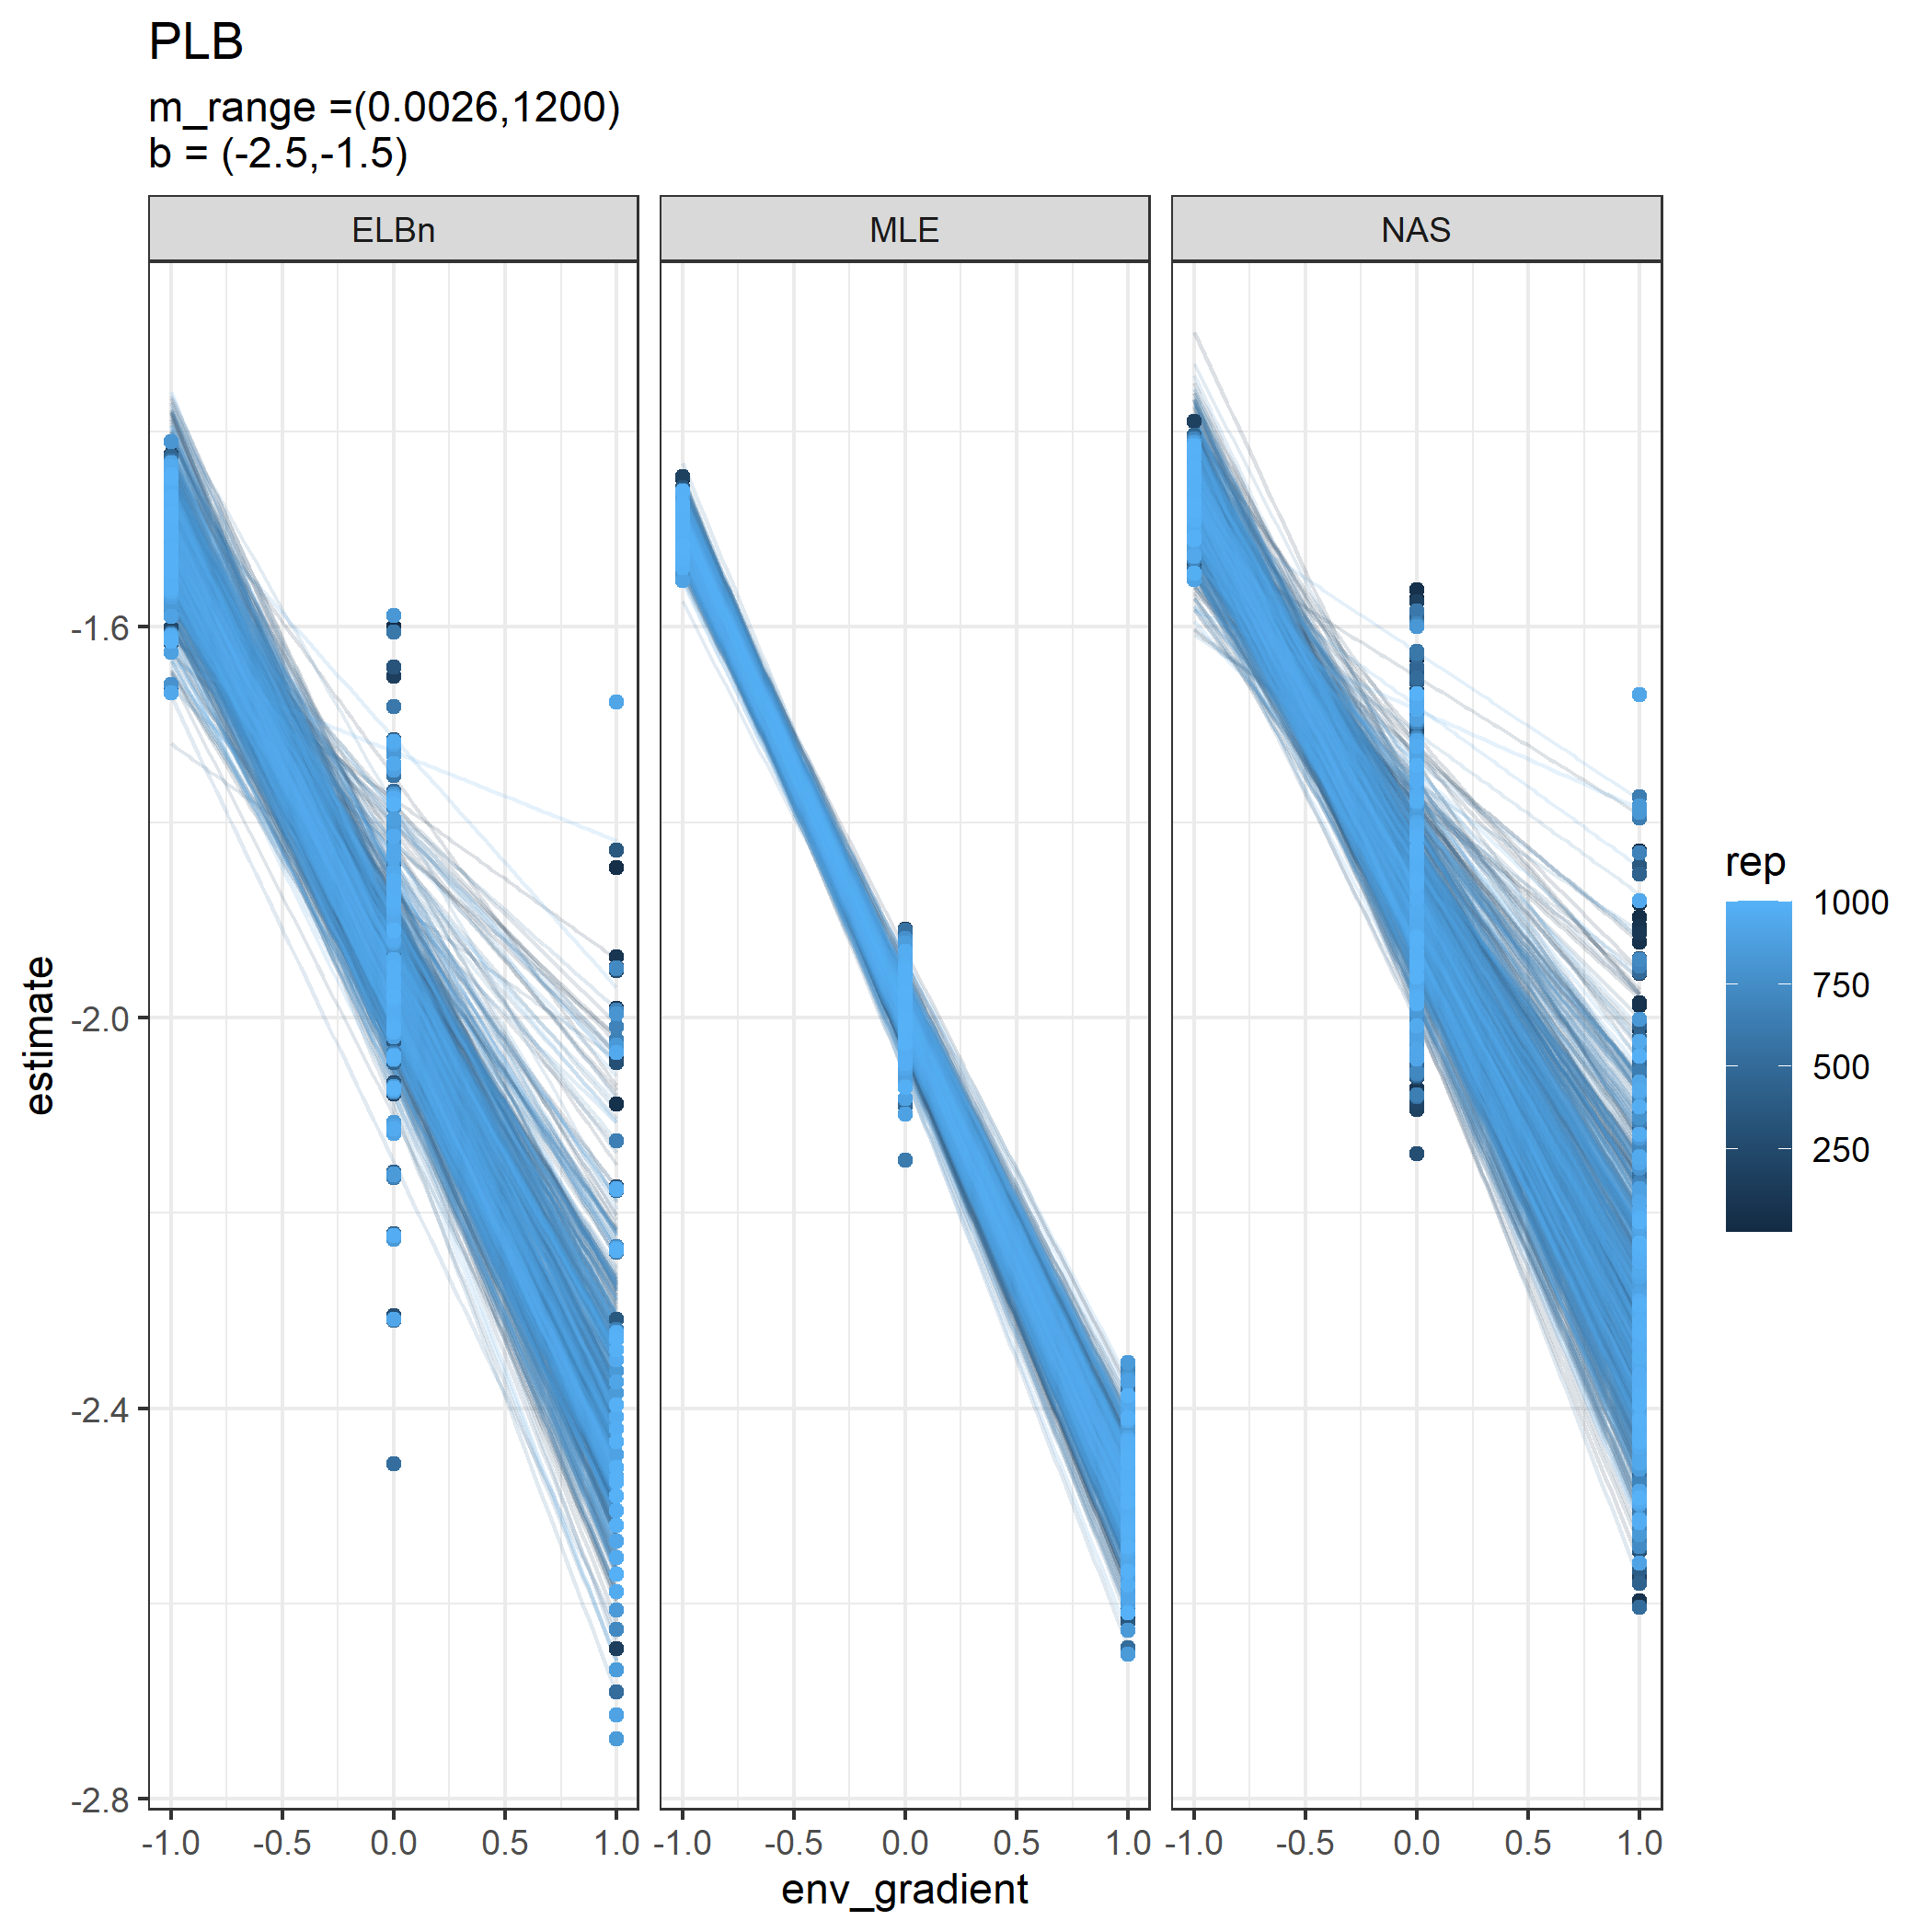
\includegraphics{figures/PLB_3_sites_main.png}
\caption{Individual regressions for three sites across a hypothetical
gradient with a known relationship of 0.5. All other parameters are the
same as in the main analysis.}
\end{figure}

\newpage

\begin{figure}
\centering
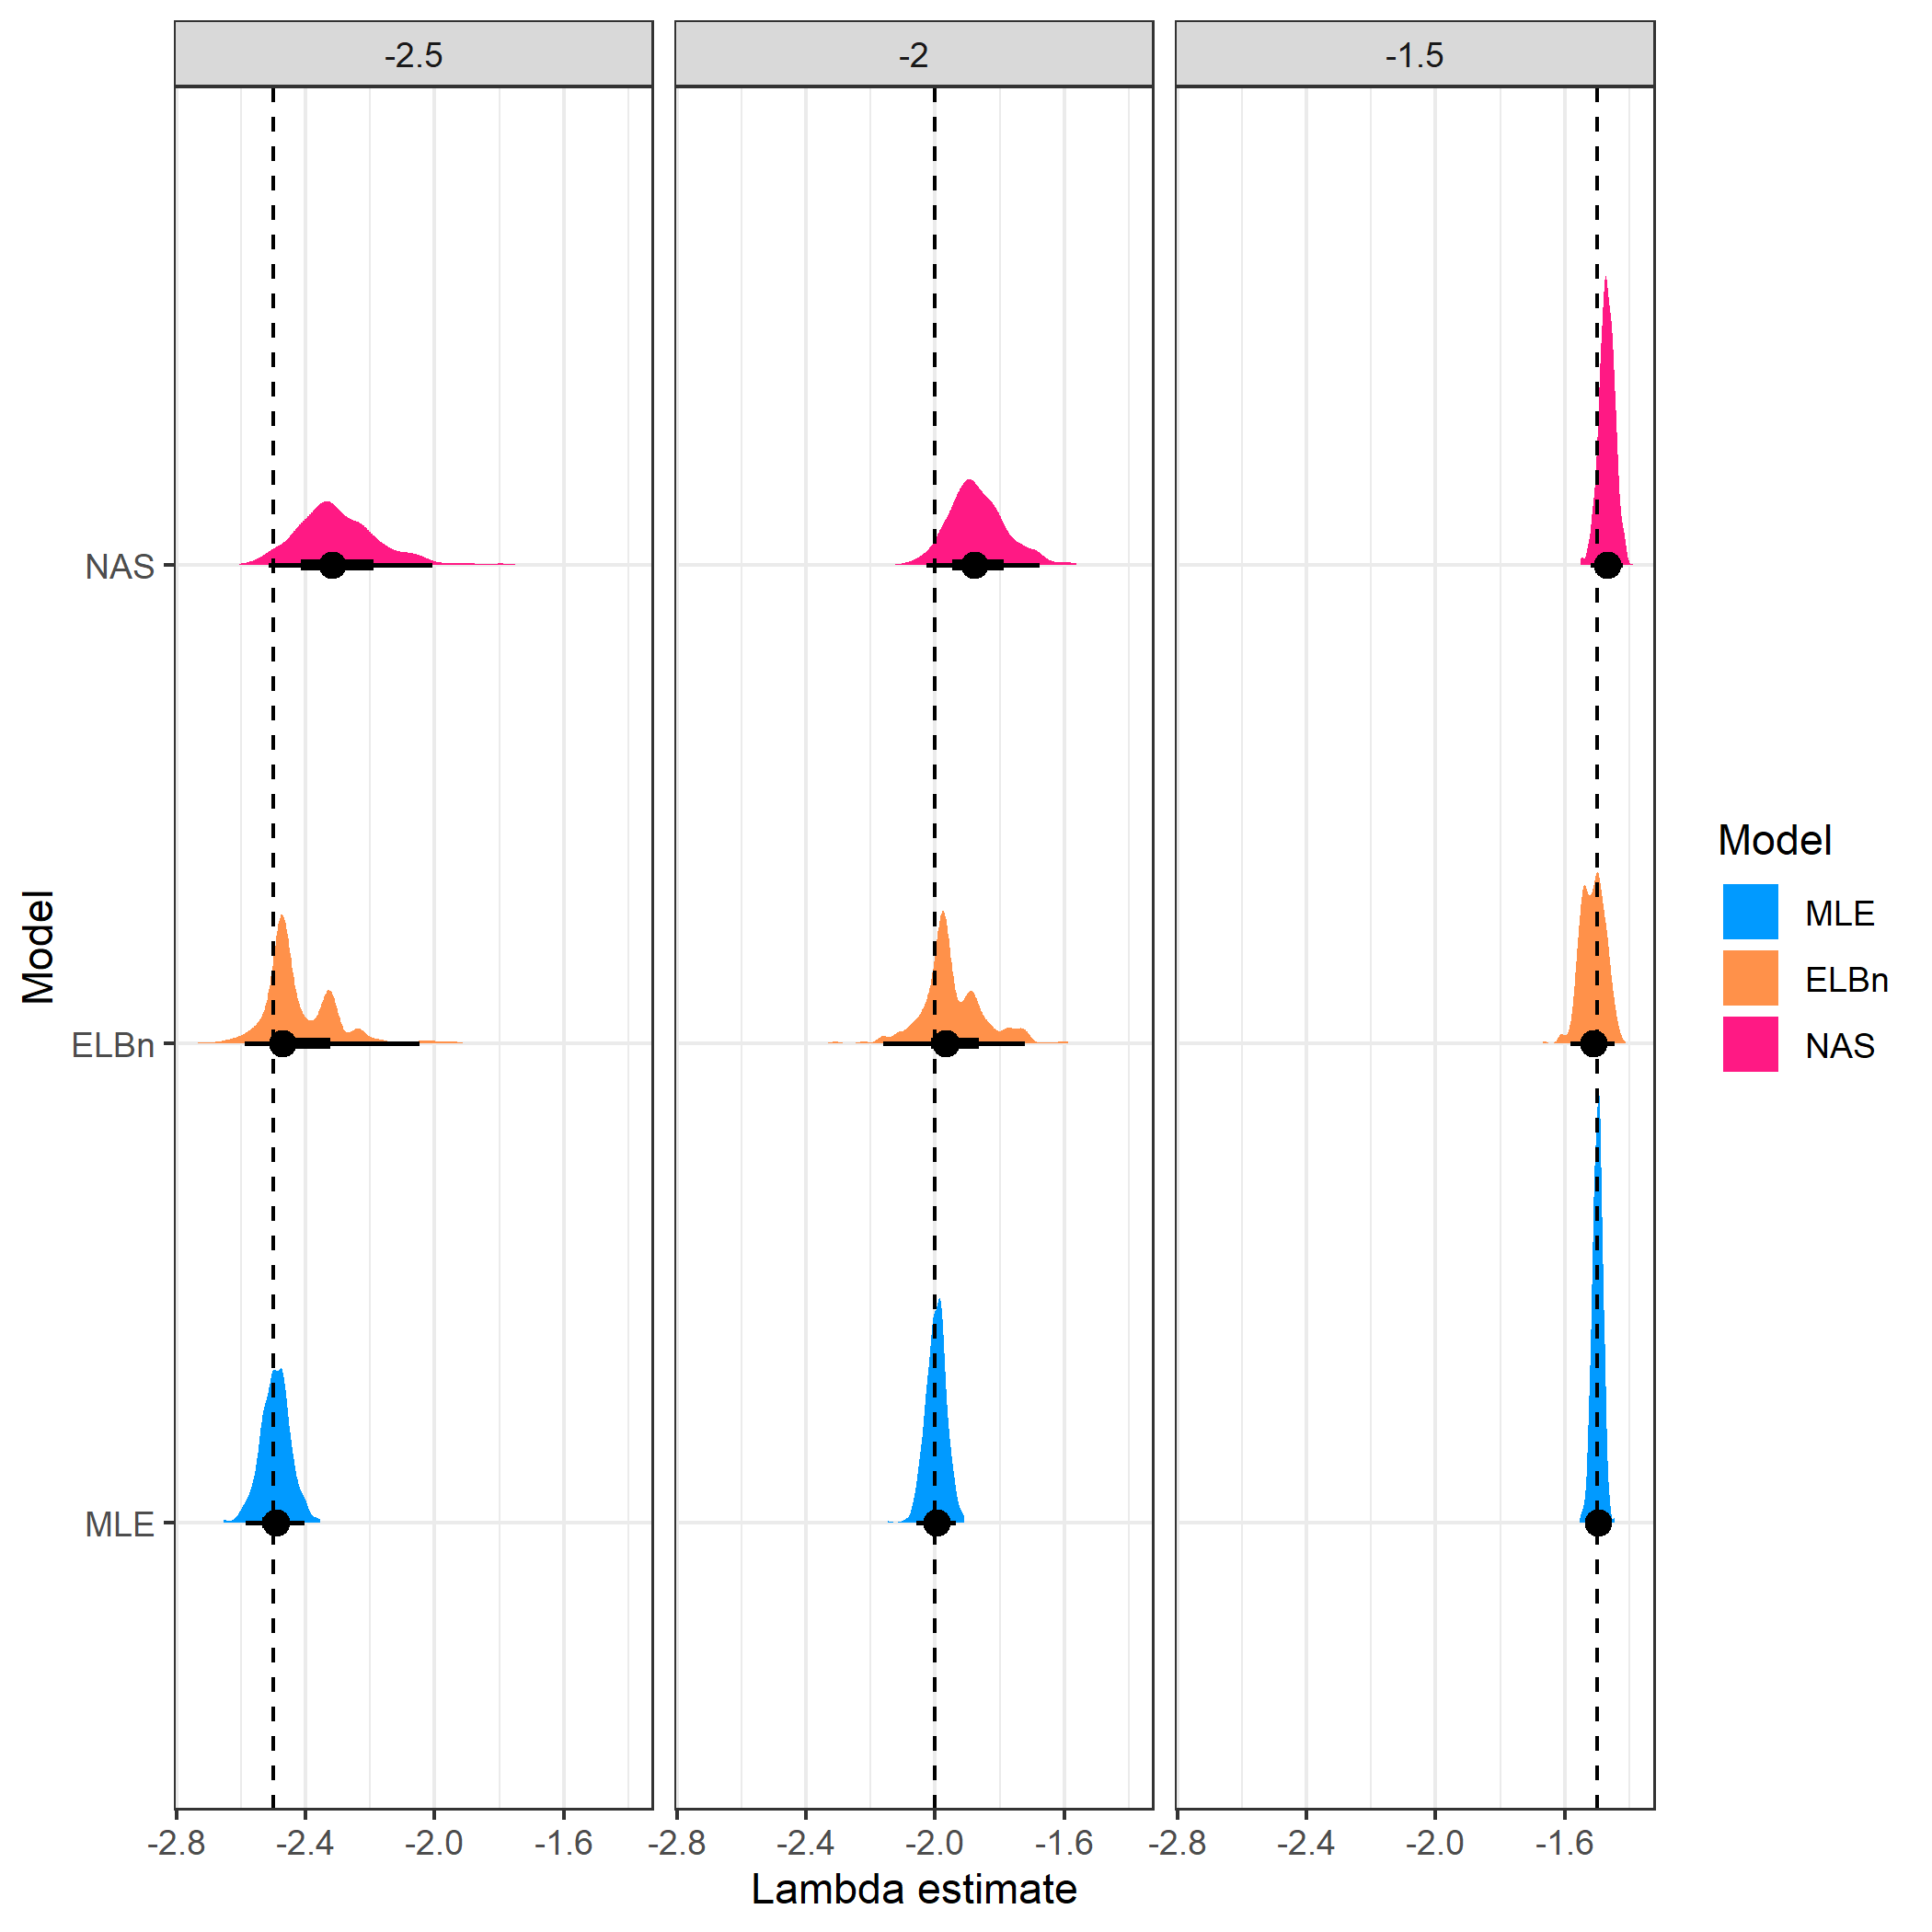
\includegraphics{figures/PLB_3_sites_est_b_density.png}
\caption{Distribution of estimated \(\lambda\) coefficient for three
sites across a hypothetical gradient with known values. All other
parameters are the same as in the main analysis.}
\end{figure}

\newpage

\begin{figure}
\centering
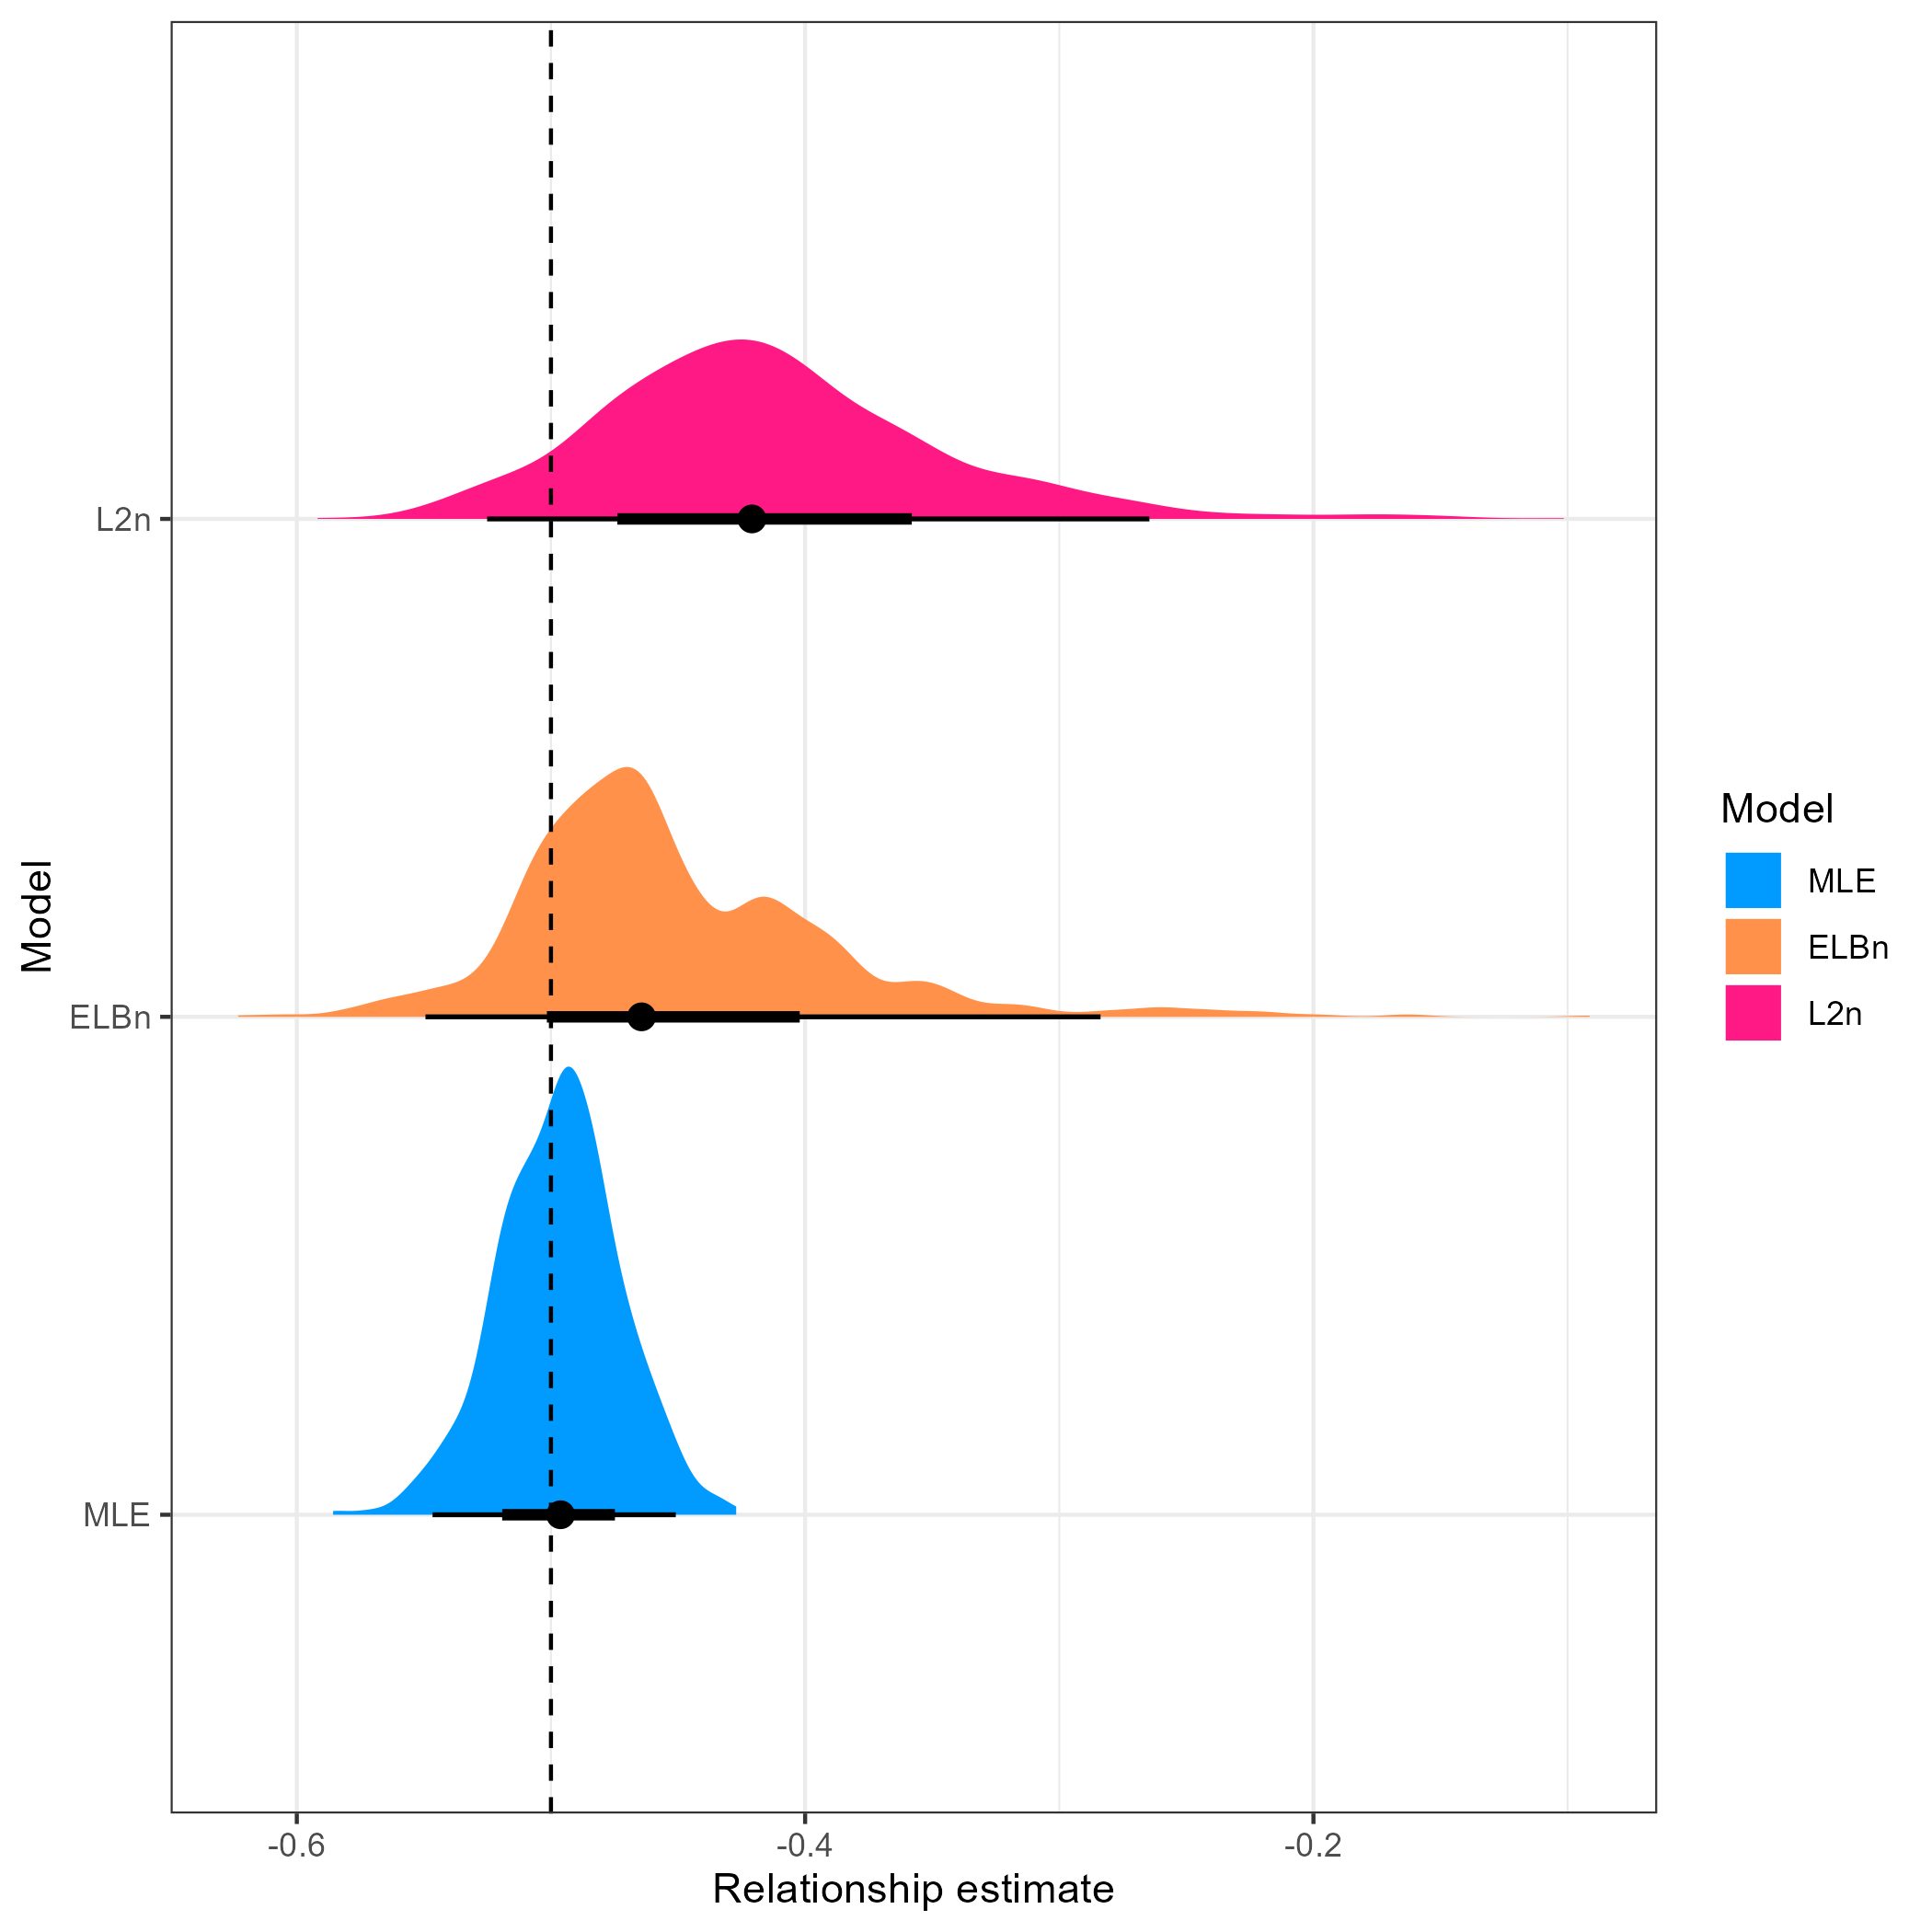
\includegraphics{figures/PLB_3_sites_relationship_density.png}
\caption{Distribution of estimated relationship (\(\beta_1\))
coefficient's for three sites across a hypothetical gradient with known
value of 0.5. All other parameters are the same as in the main analysis}
\end{figure}

\newpage

\hypertarget{sample-size}{%
\subsection{Sample size}\label{sample-size}}

\begin{figure}
\centering
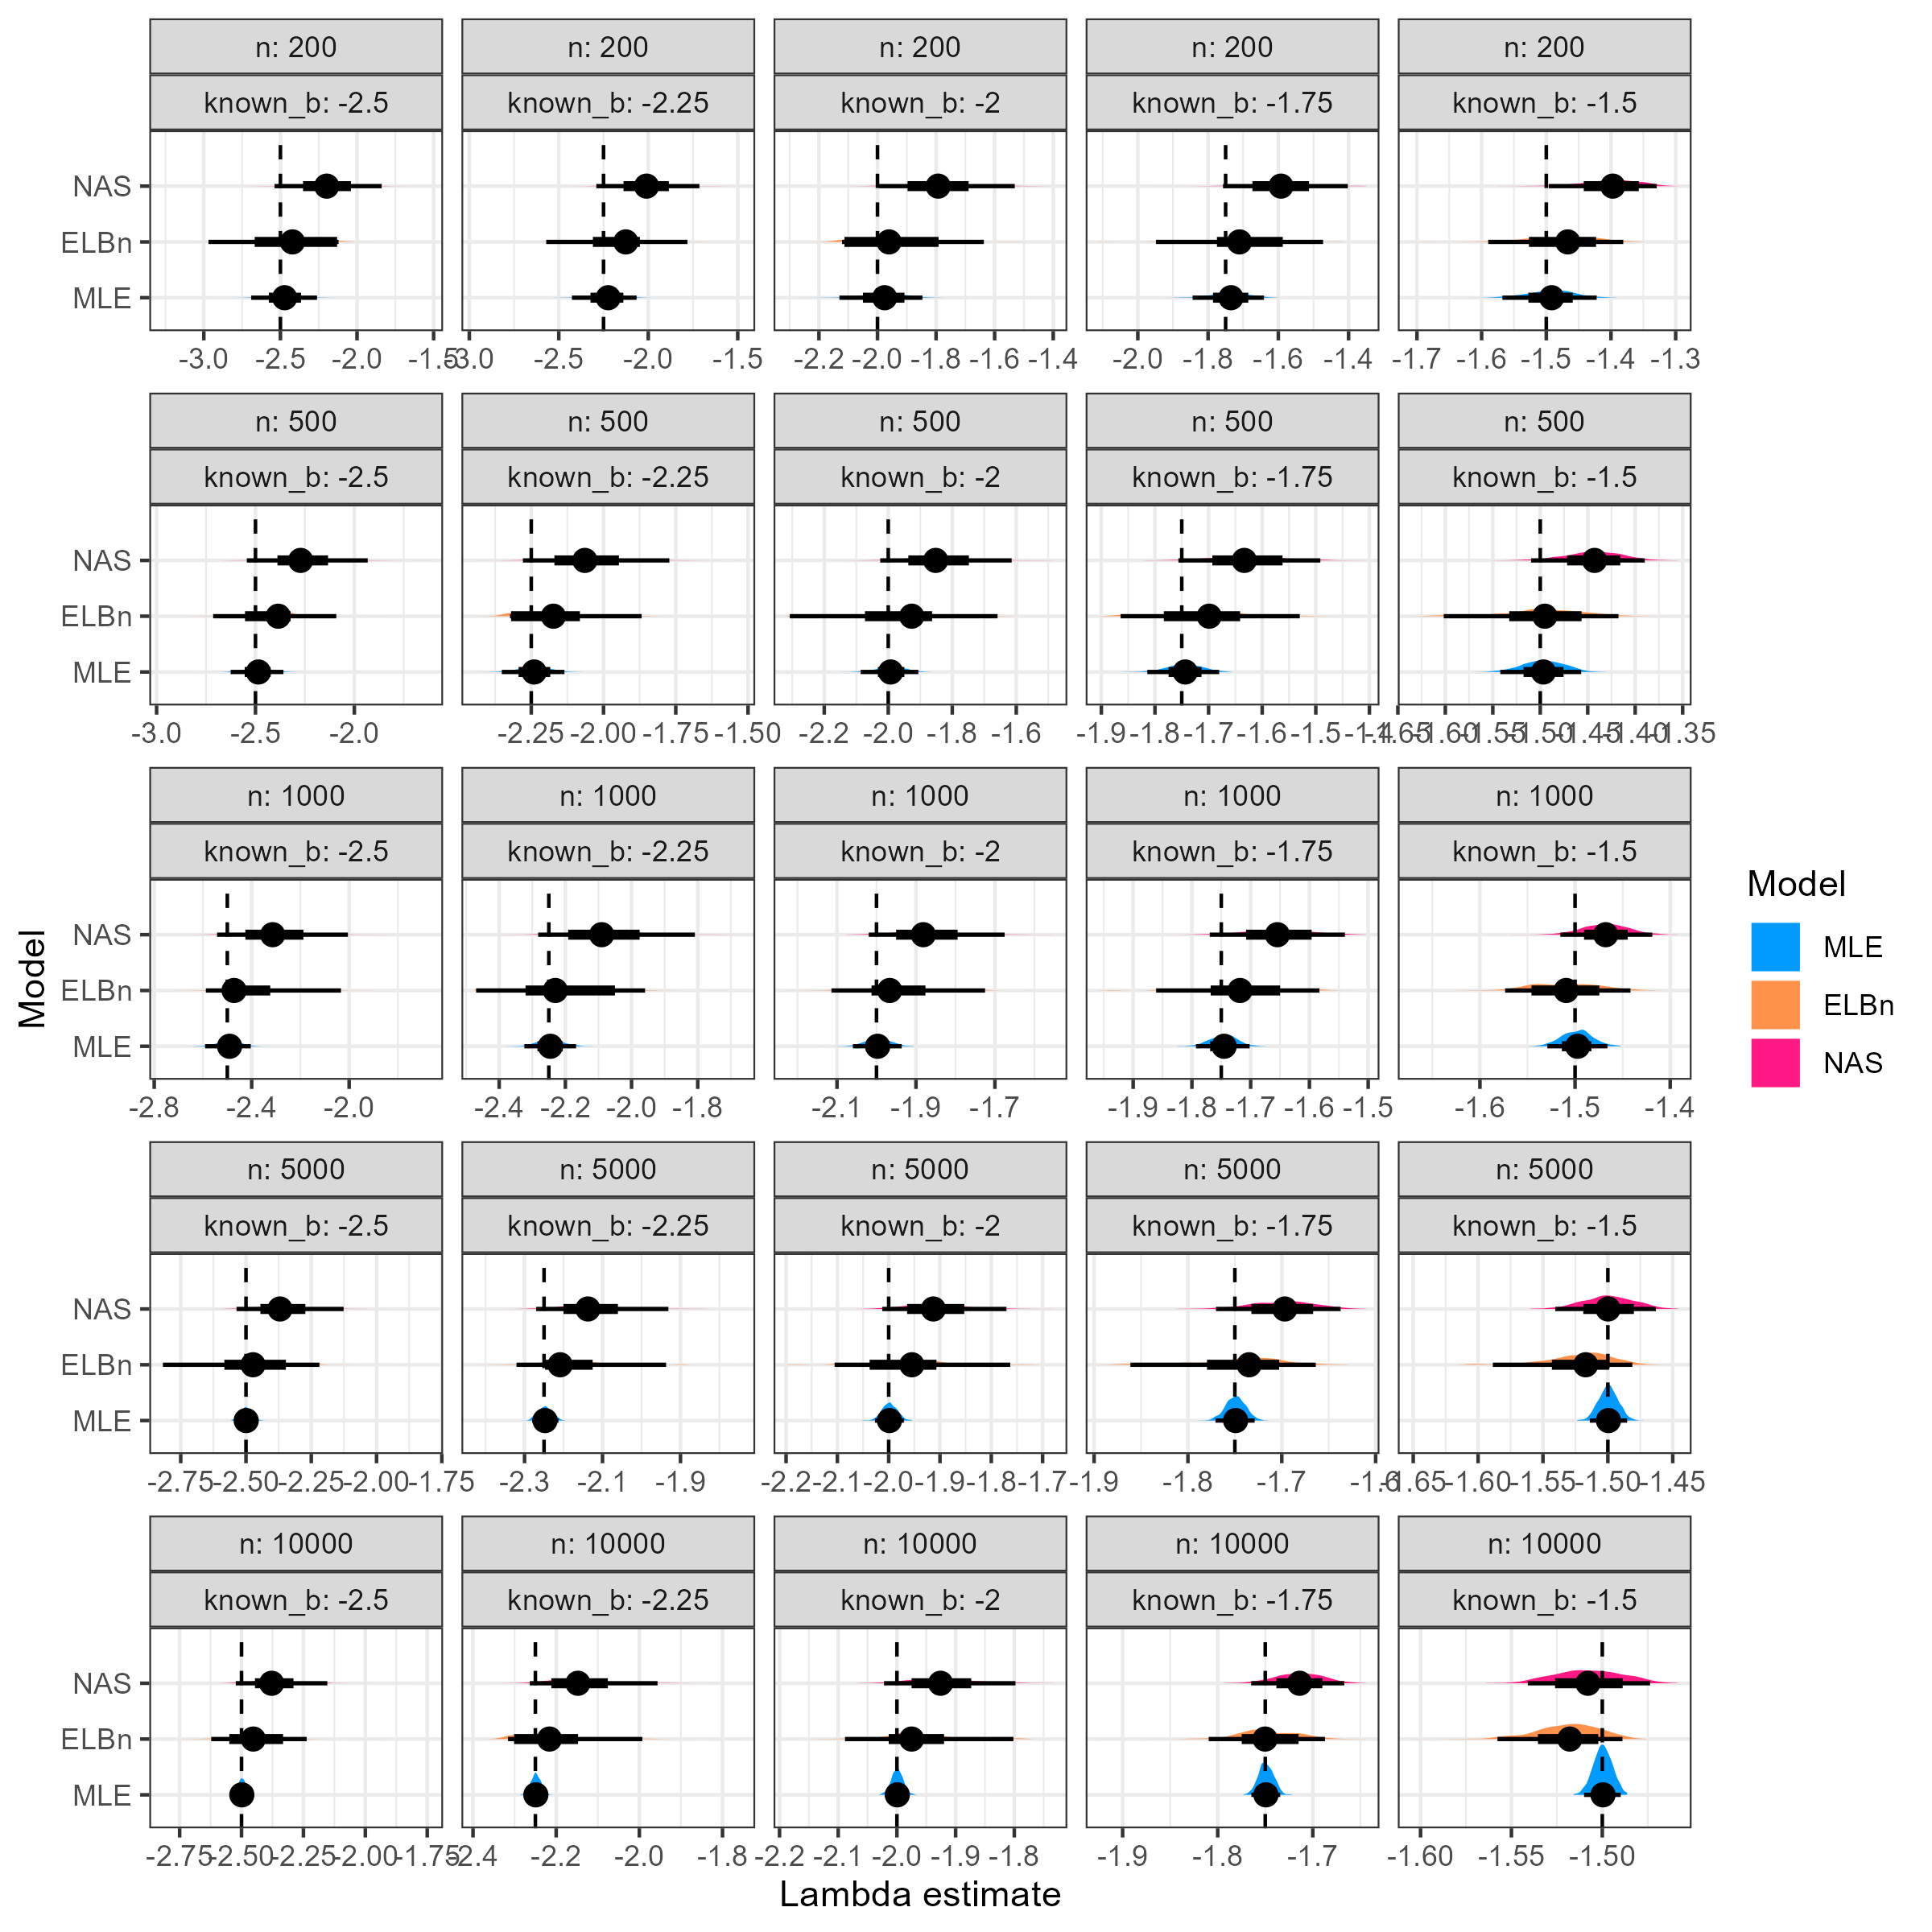
\includegraphics{figures/n_vary_est_b.png}
\caption{Distribution of size spectra parameter estimates. Vertical line
is the known parameter (dashed line) wich describes the bounded power
law distribution from which the body size estimates were sampled. As n
increases (top to bottom) and \(\lambda\) increases (left to right), the
accuracy of the estimate improves across all methods.}
\end{figure}

\newpage

\begin{figure}
\centering
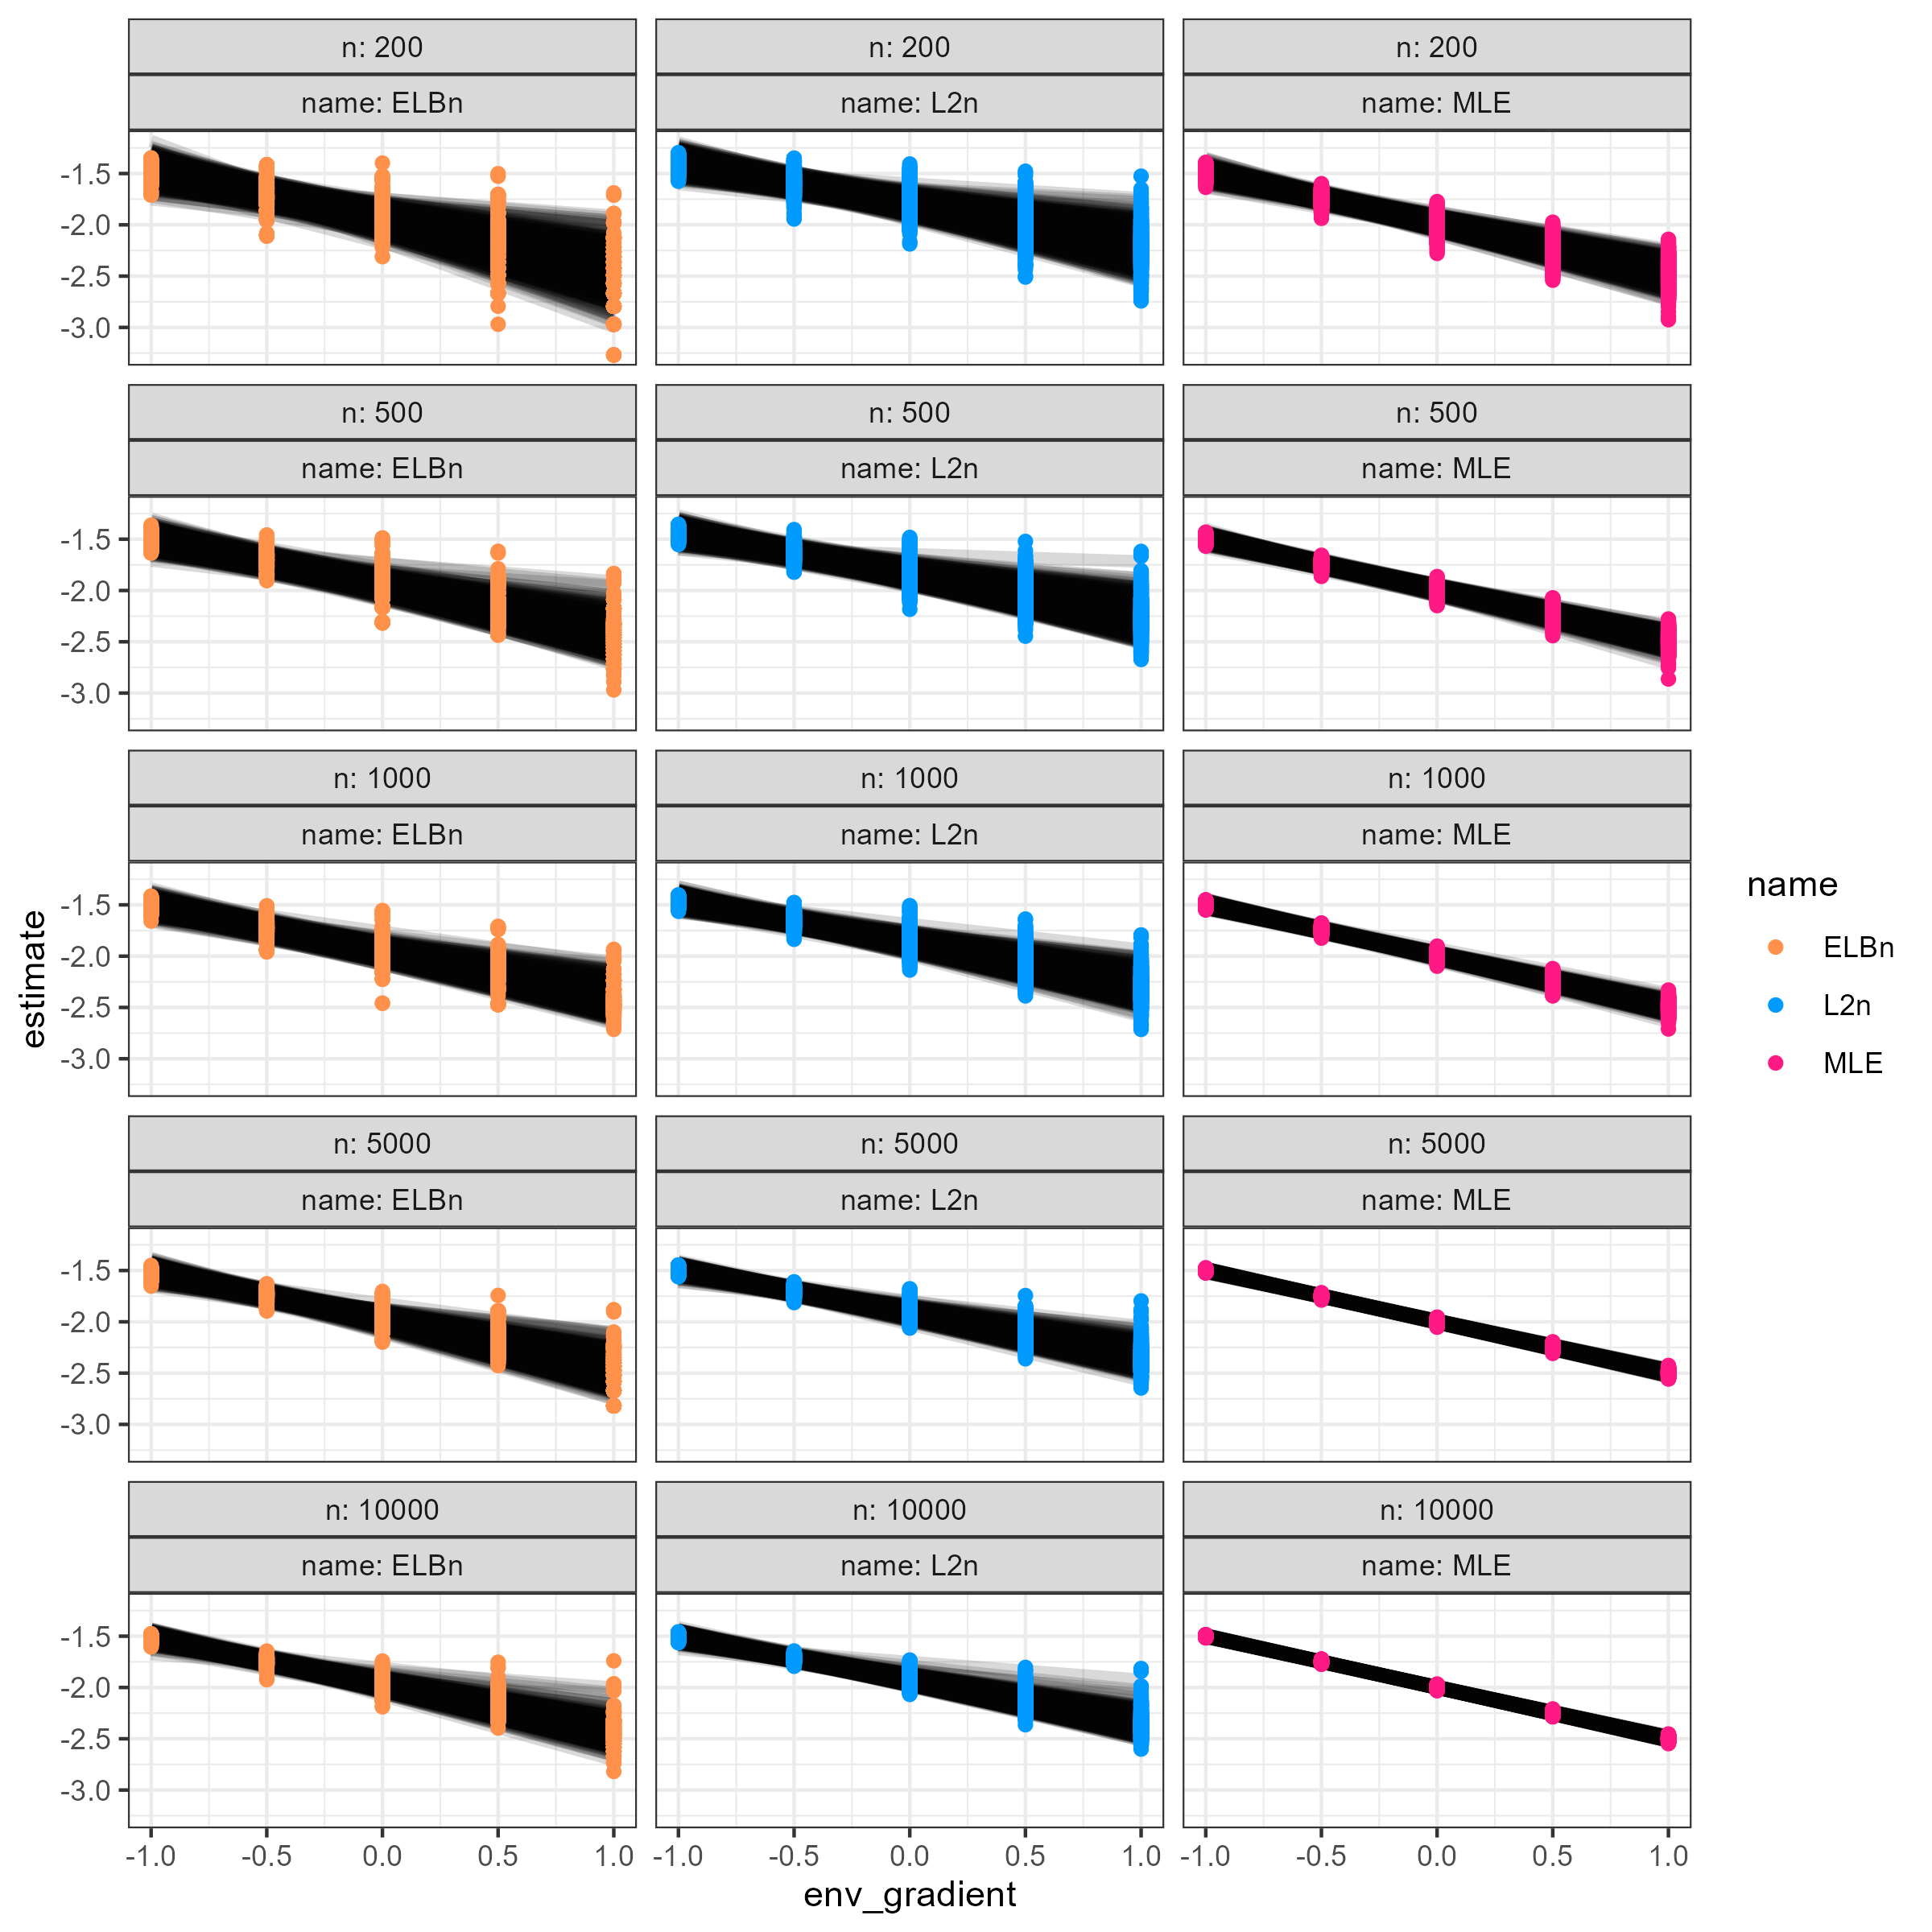
\includegraphics{figures/n_vary_main.png}
\caption{Individual regressions when varying sample size}
\end{figure}

\newpage

\begin{figure}
\centering
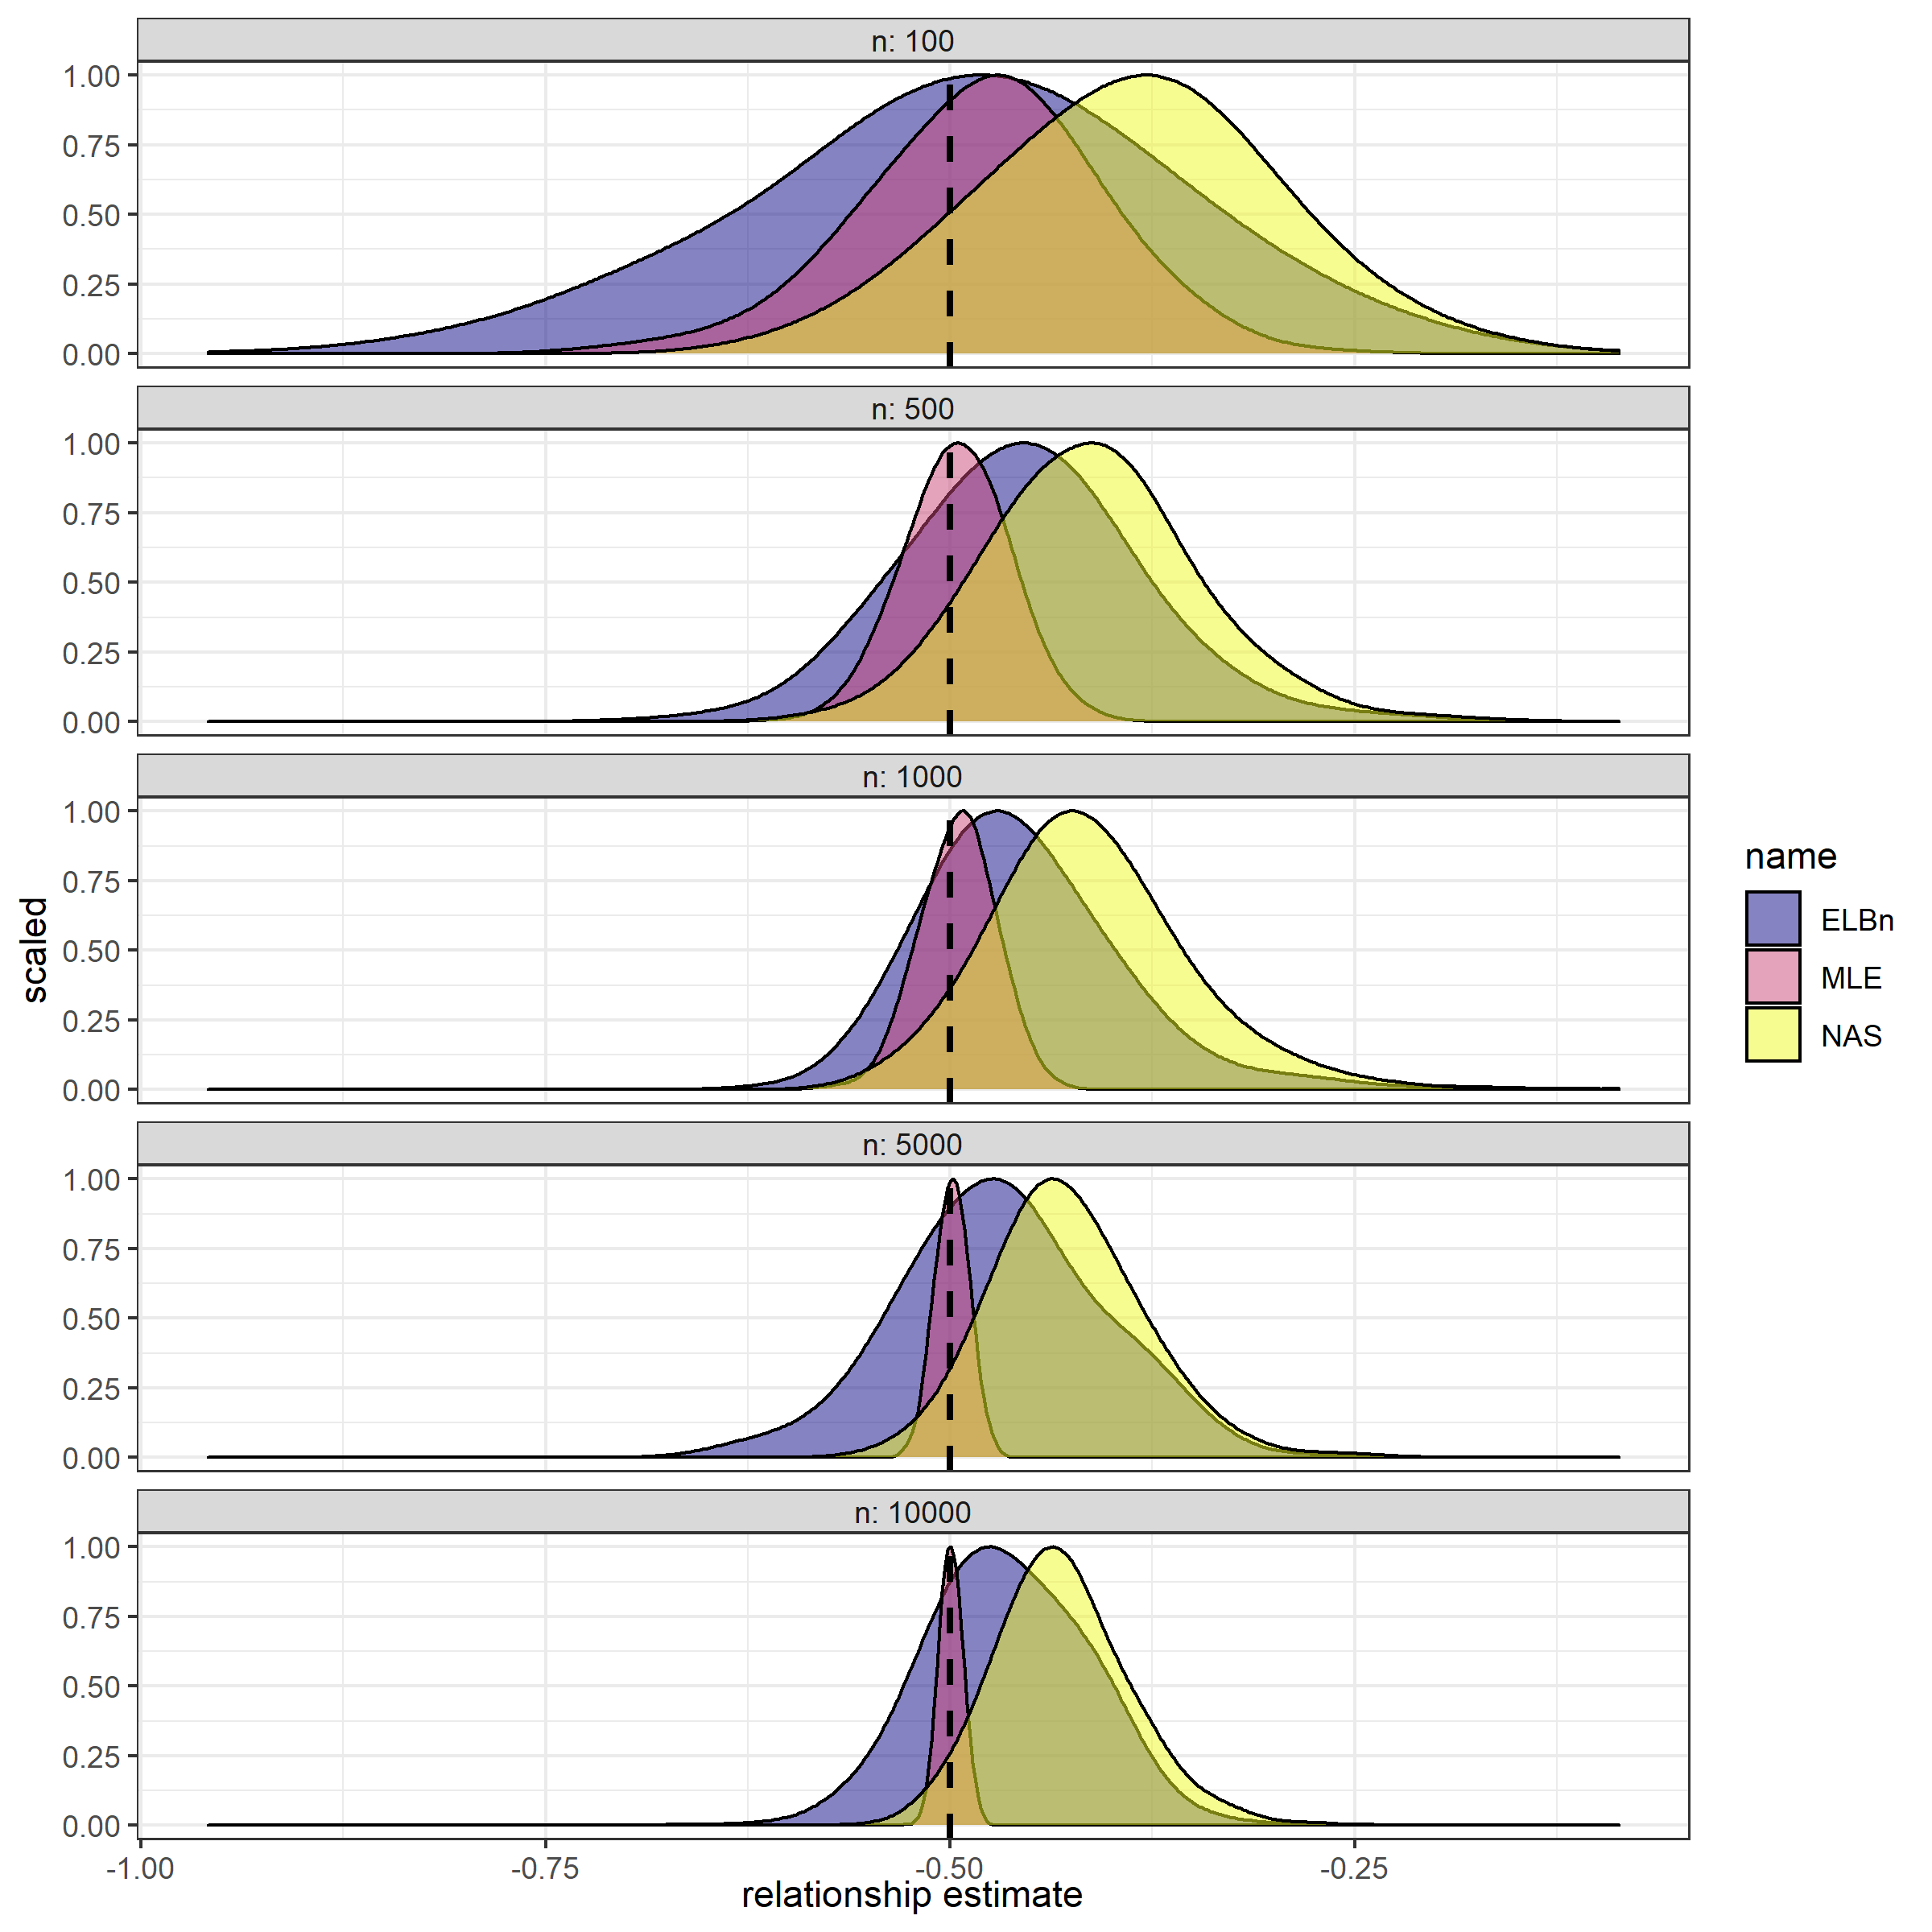
\includegraphics{figures/n_vary_relationship_density.png}
\caption{Distribtuion of the relationship coefficients with varying
sample size}
\end{figure}

\newpage

\hypertarget{lambda-and-relationship-estimates}{%
\subsection{\texorpdfstring{\(\lambda\) and relationship
estimates}{\textbackslash lambda and relationship estimates}}\label{lambda-and-relationship-estimates}}

\textbf{NOTE} I'm considering dropping the \(\lambda\) estimate plots
from the manuscript. I think it's too much info, but if it adds to the
story I'm happy to leave it in. \textbf{END}

In the main analysis, we simulate body size data from bounded power law
distributions while varying the \(\lambda\) exponent which describes the
distribution. For the results presented in the main text, we held the
number of sites at 5, scaled the environmental gradient from -1 to 1,
and set the minimum and maximum body sizes to \(0.0026\) and
\(1.2 *10^3\) respectively. Here, we plot the results of varying the
number of sites (3, 10), increasing the scale of the environmental
gradient (-100 to 100) and decreasing the range of body sizes (min = 1,
max = 100). Generally, the results reported in the main manuscript are
robust to changing these parameters: the MLE estimate is nearly always
closer to the known parameters, and the variation in these estimates is
usually smaller than the binning methods.

\newpage

\hypertarget{number-of-sites-3}{%
\subsubsection{Number of sites = 3}\label{number-of-sites-3}}

\begin{figure}
\centering
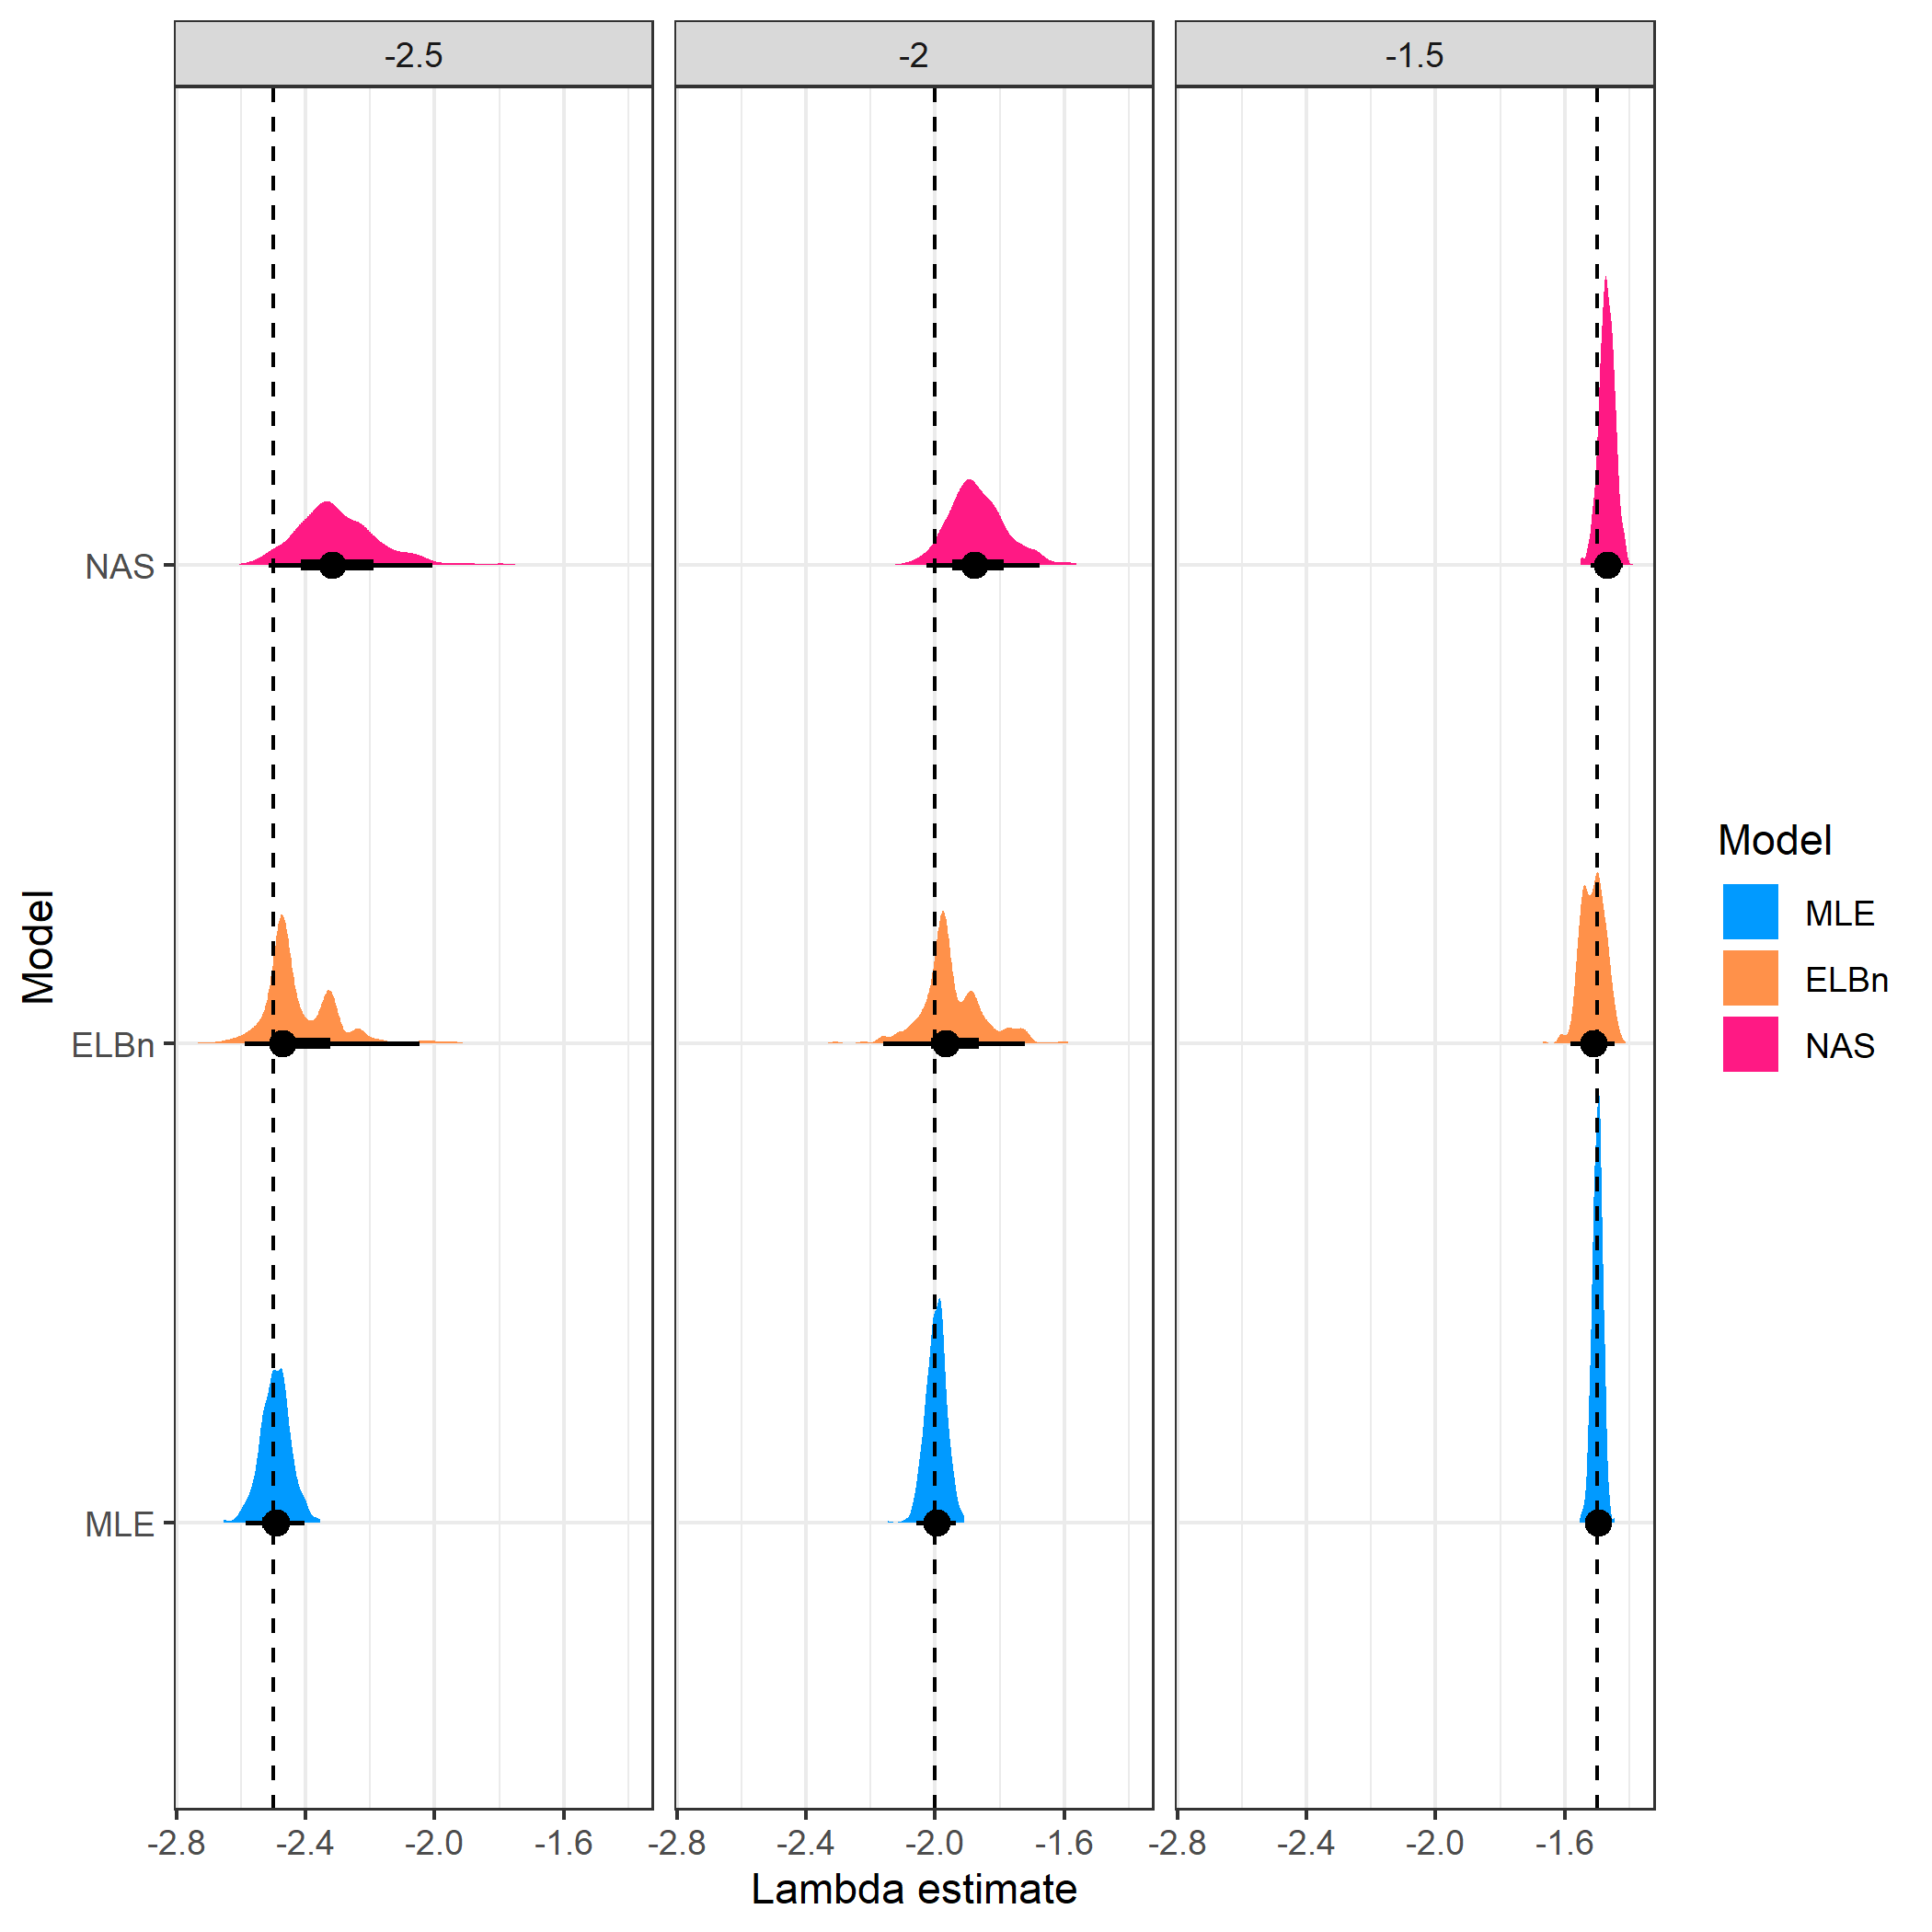
\includegraphics{figures/PLB_3_sites_est_b_density.png}
\caption{Distribution of estimated \(\lambda\) coefficient across a
hypothetical gradient with known values (dashed line). The number of
sites is reduced to 3, compared with 5 sites presented in the main
anaysis.}
\end{figure}

\newpage

\begin{figure}
\centering
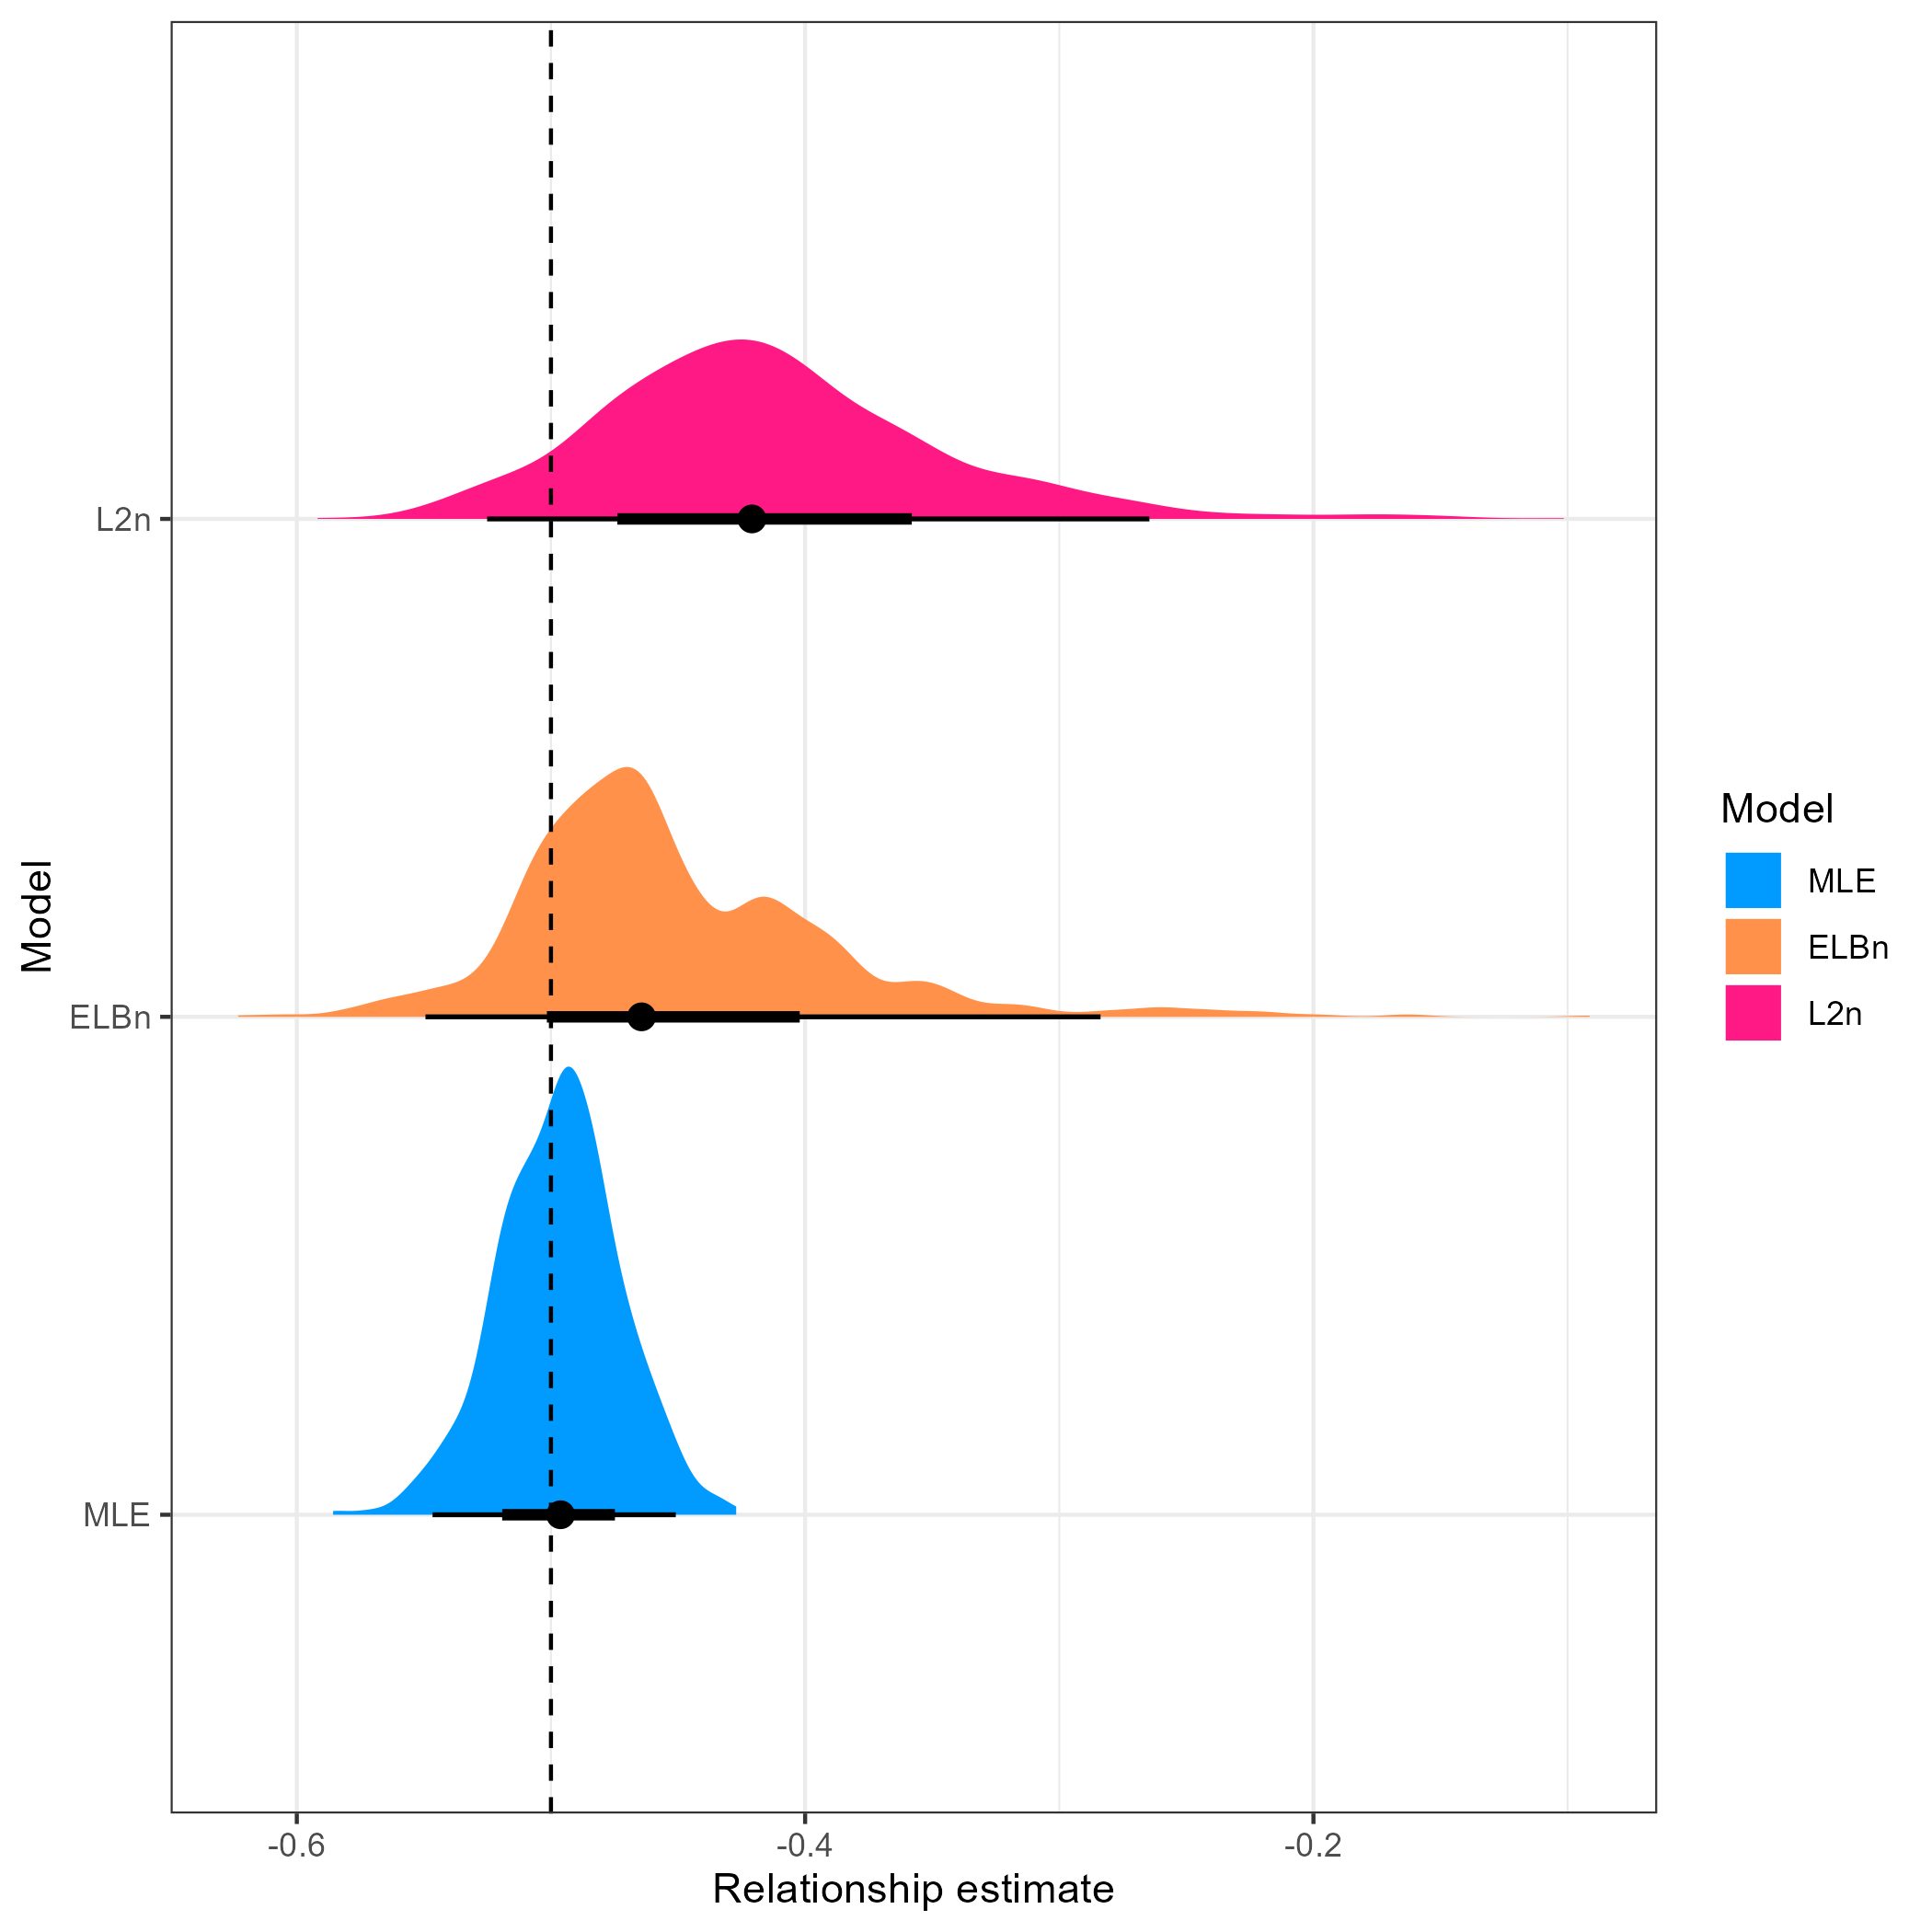
\includegraphics{figures/PLB_3_sites_relationship_density.png}
\caption{Relationship estimate}
\end{figure}

\newpage

\hypertarget{number-of-sites-10}{%
\subsubsection{Number of sites = 10}\label{number-of-sites-10}}

\begin{figure}
\centering
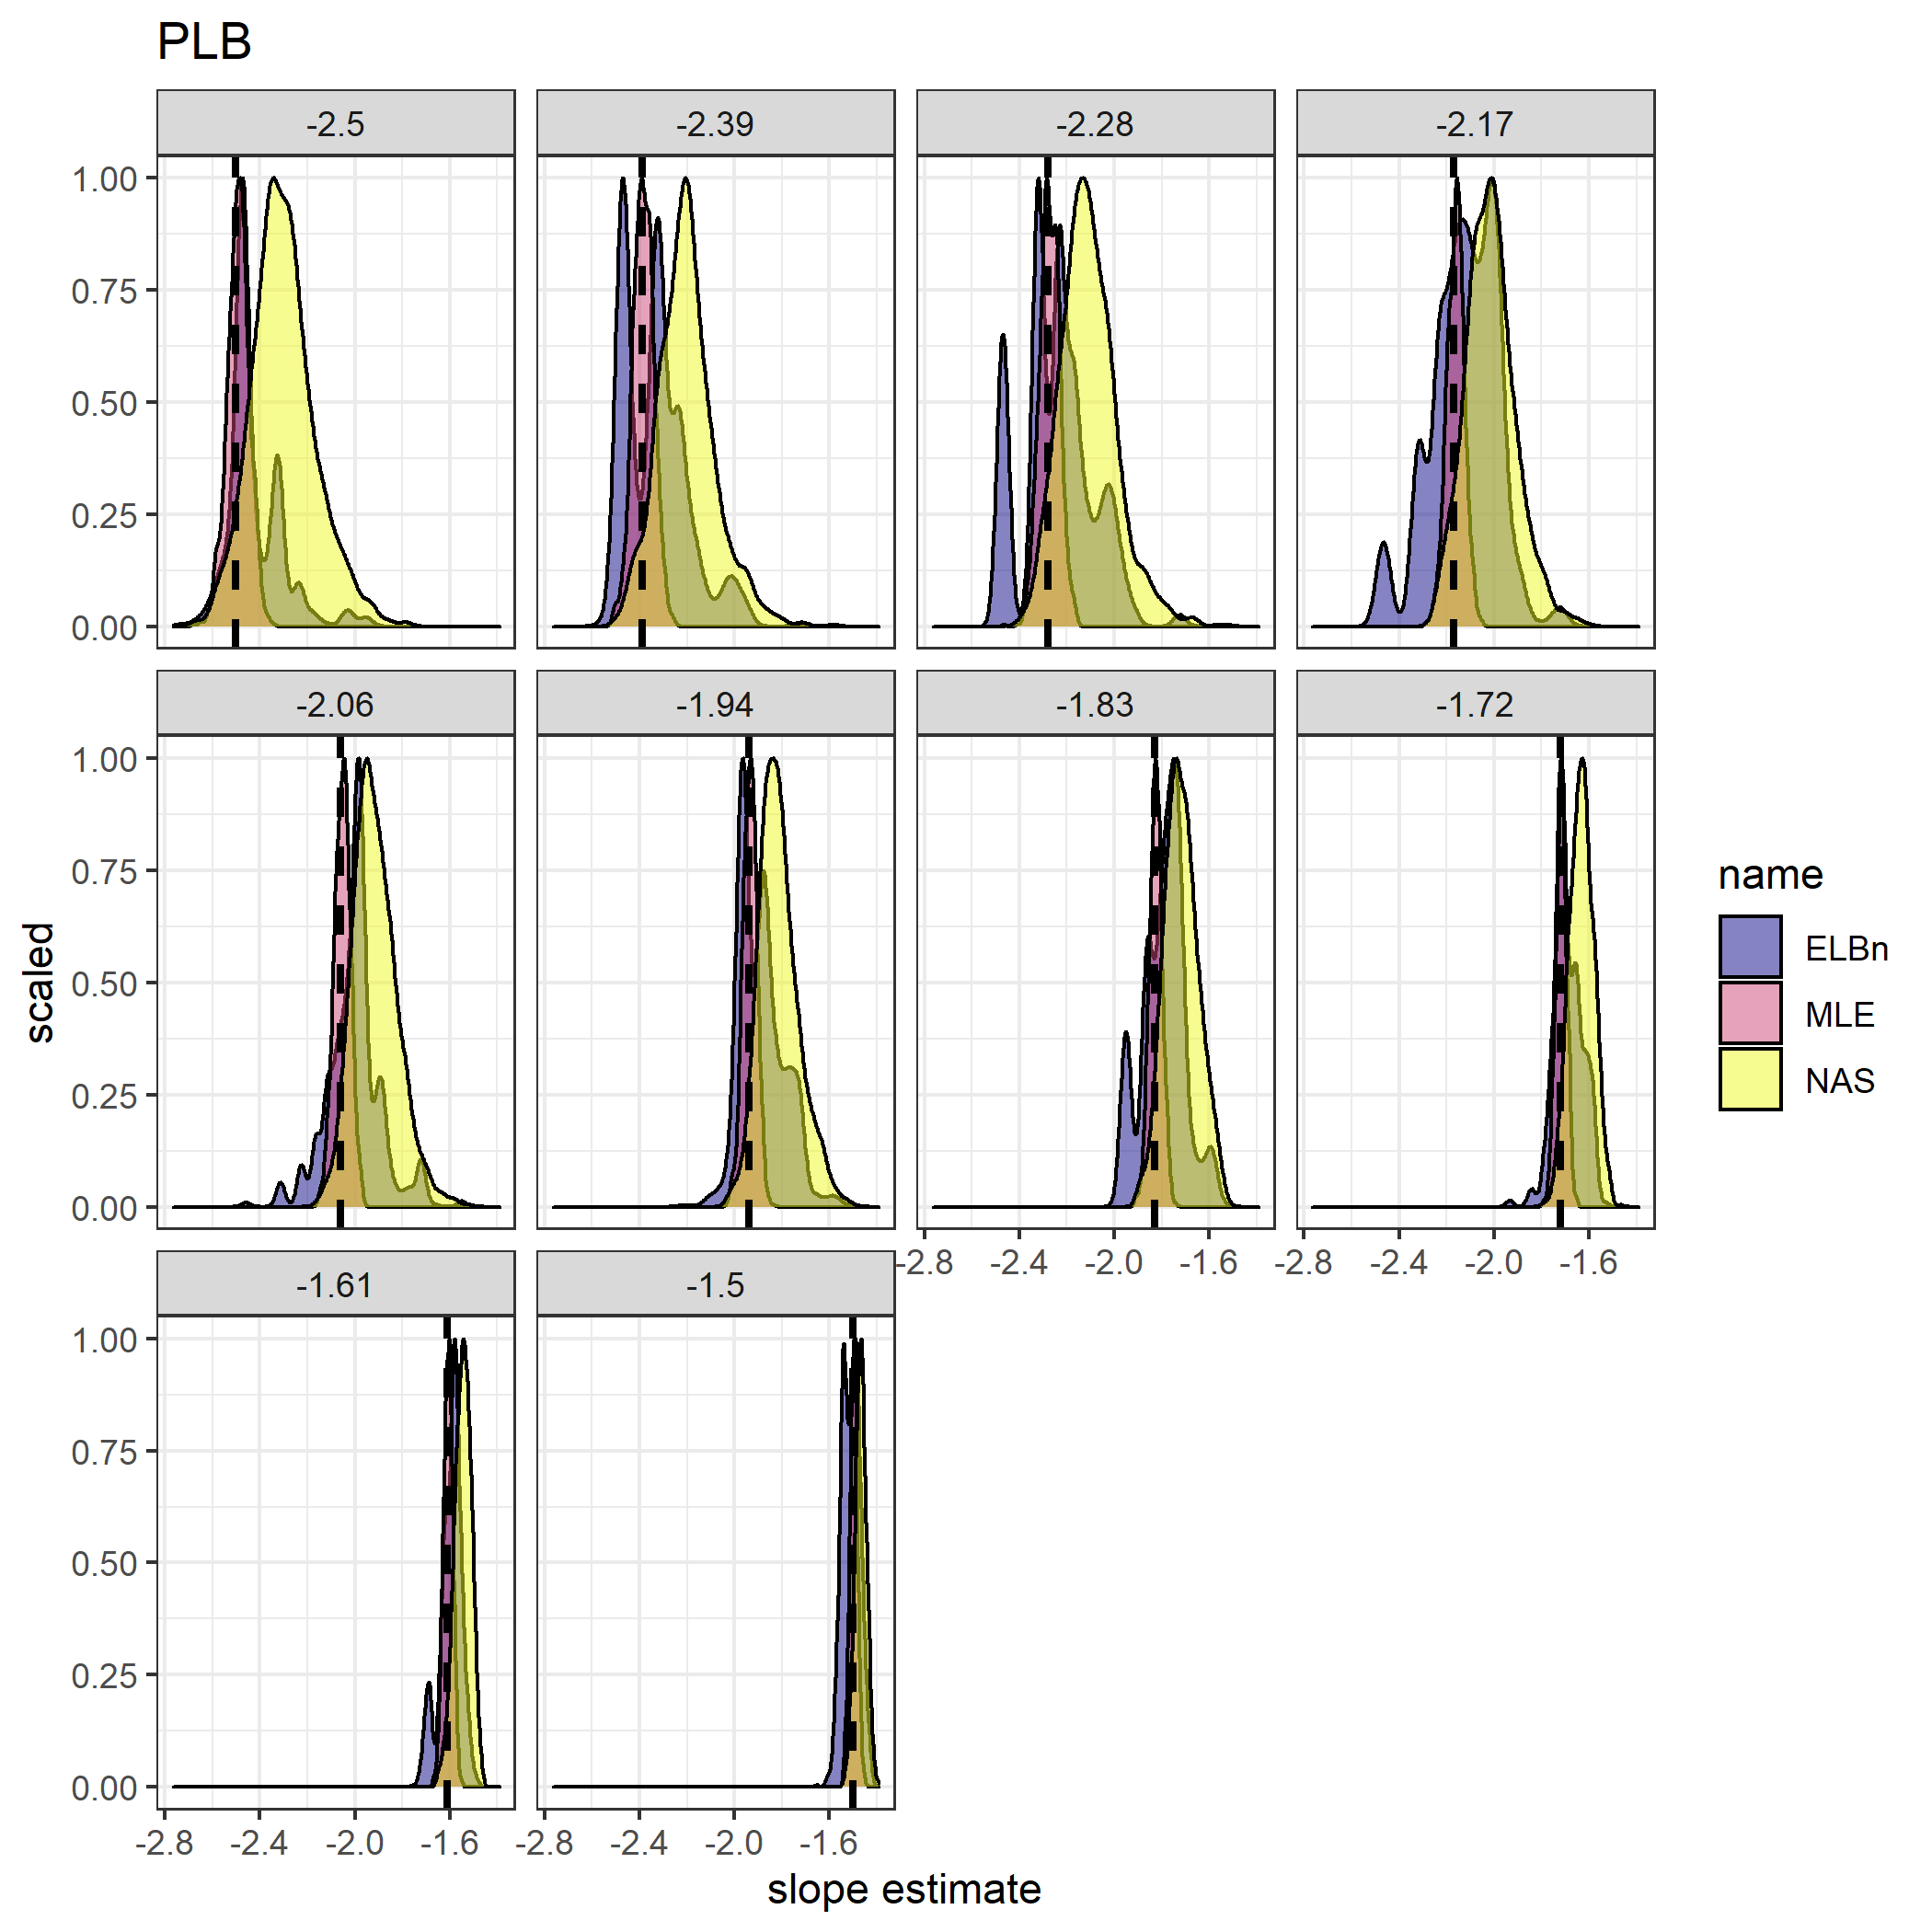
\includegraphics{figures/PLB_10_sites_est_b_density.png}
\caption{Distribution of estimated \(\lambda\) coefficient across a
hypothetical gradient with known values(dashed line). The number of
sites is increased to 10, compared with 5 sites presented in the main
anaysis.}
\end{figure}

\newpage

\begin{figure}
\centering
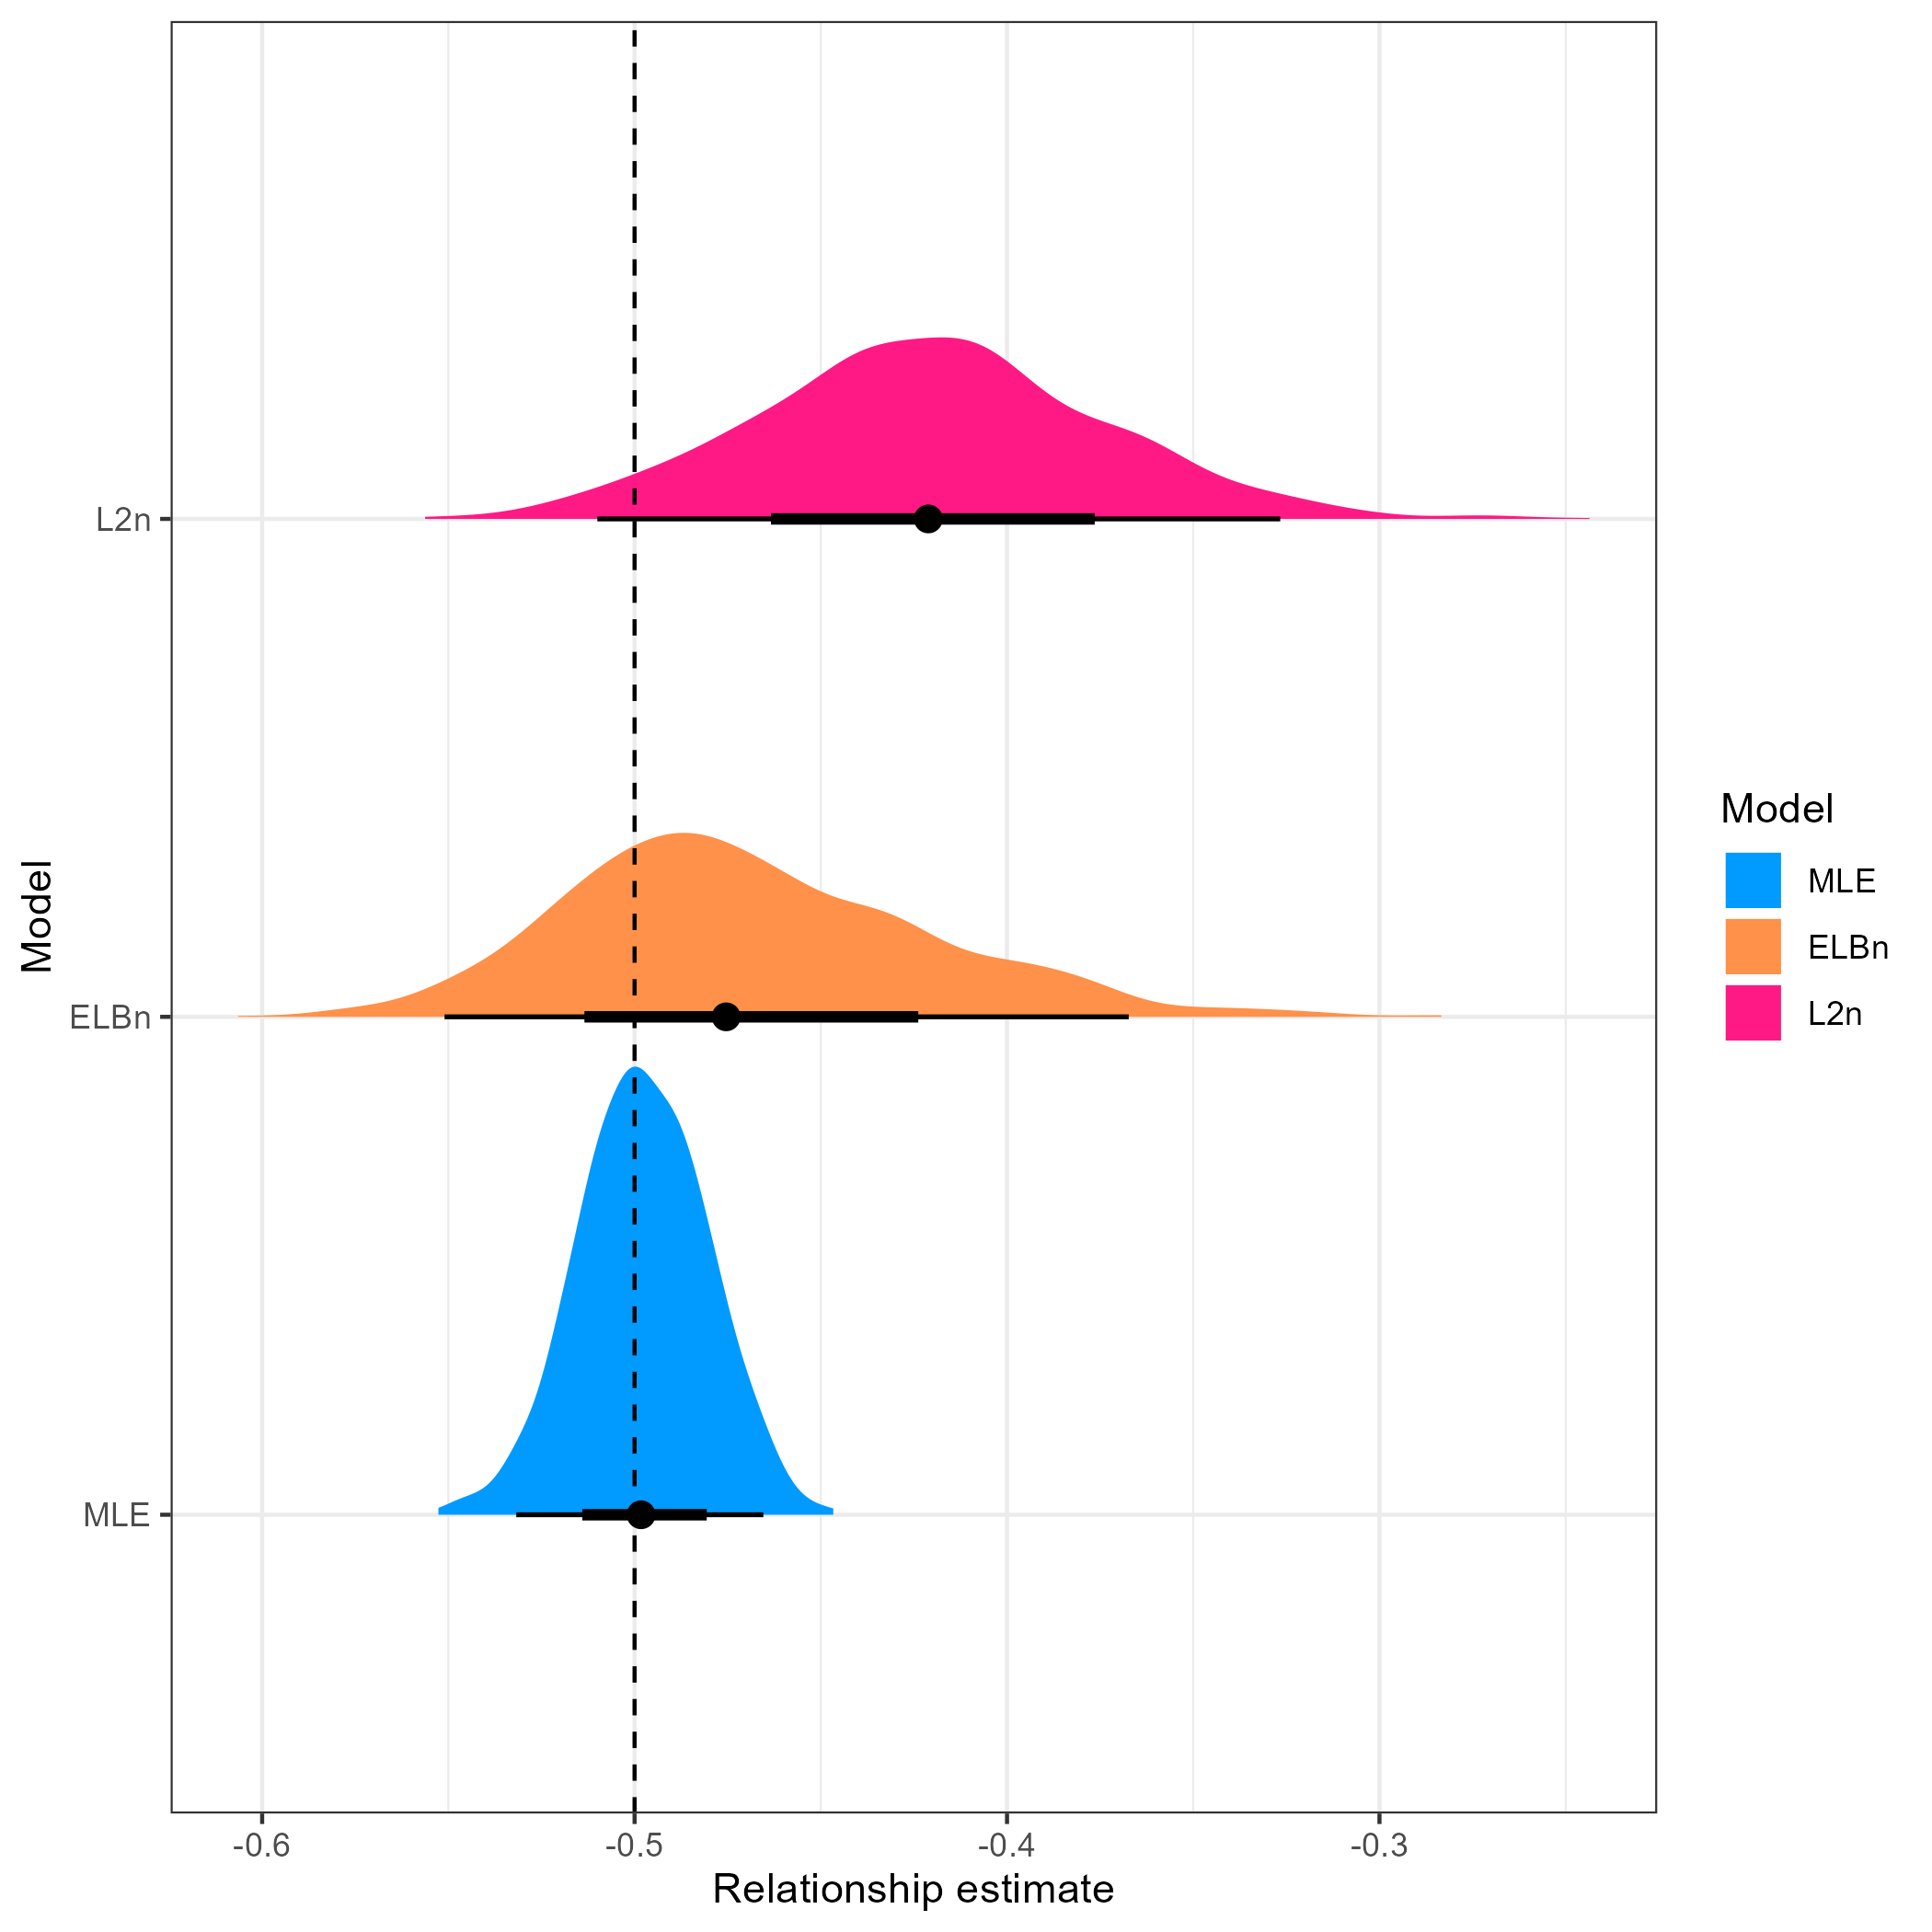
\includegraphics{figures/PLB_10_sites_relationship_density.png}
\caption{Relationship estimate}
\end{figure}

\newpage

\hypertarget{environmental-gradient}{%
\subsubsection{Environmental Gradient}\label{environmental-gradient}}

\begin{figure}
\centering
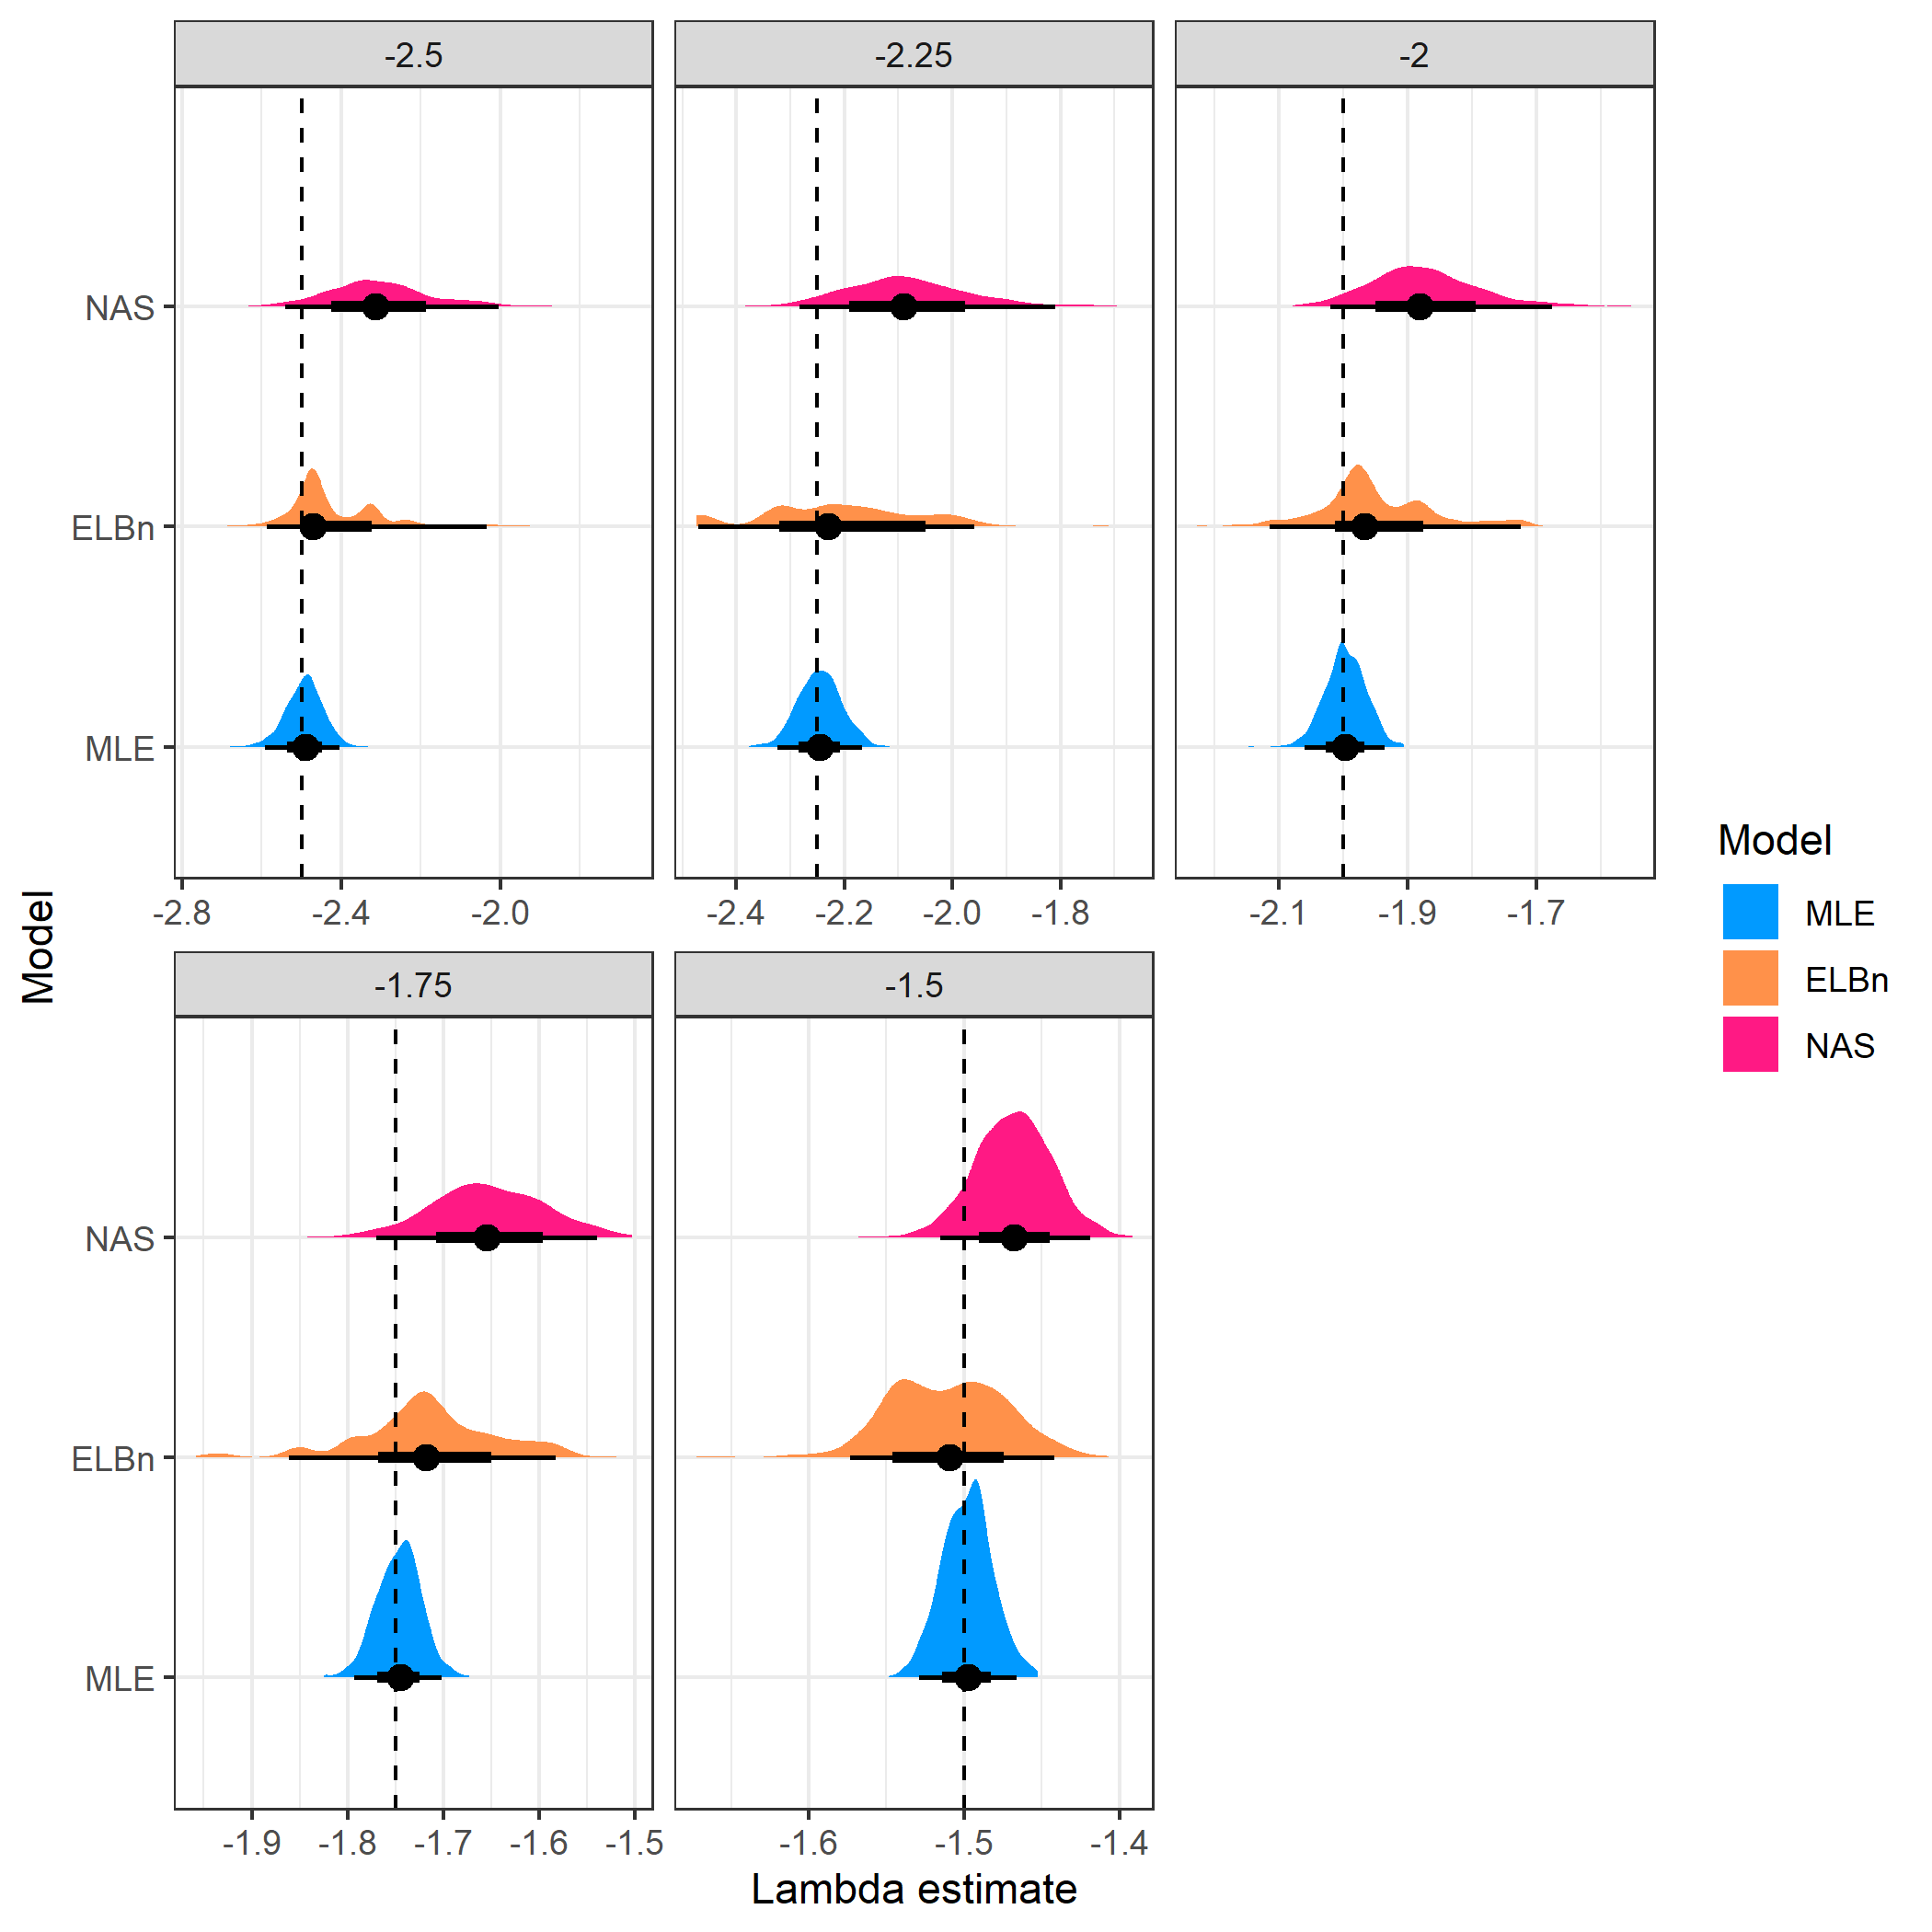
\includegraphics{figures/PLB_large_x_est_b_density.png}
\caption{Distribution of estimated \(\lambda\) coefficient for five
sites across a hypothetical gradient with known values (dashed line).
The range of the environmental gradient was increased (-100 to 100).}
\end{figure}

\newpage

\begin{figure}
\centering
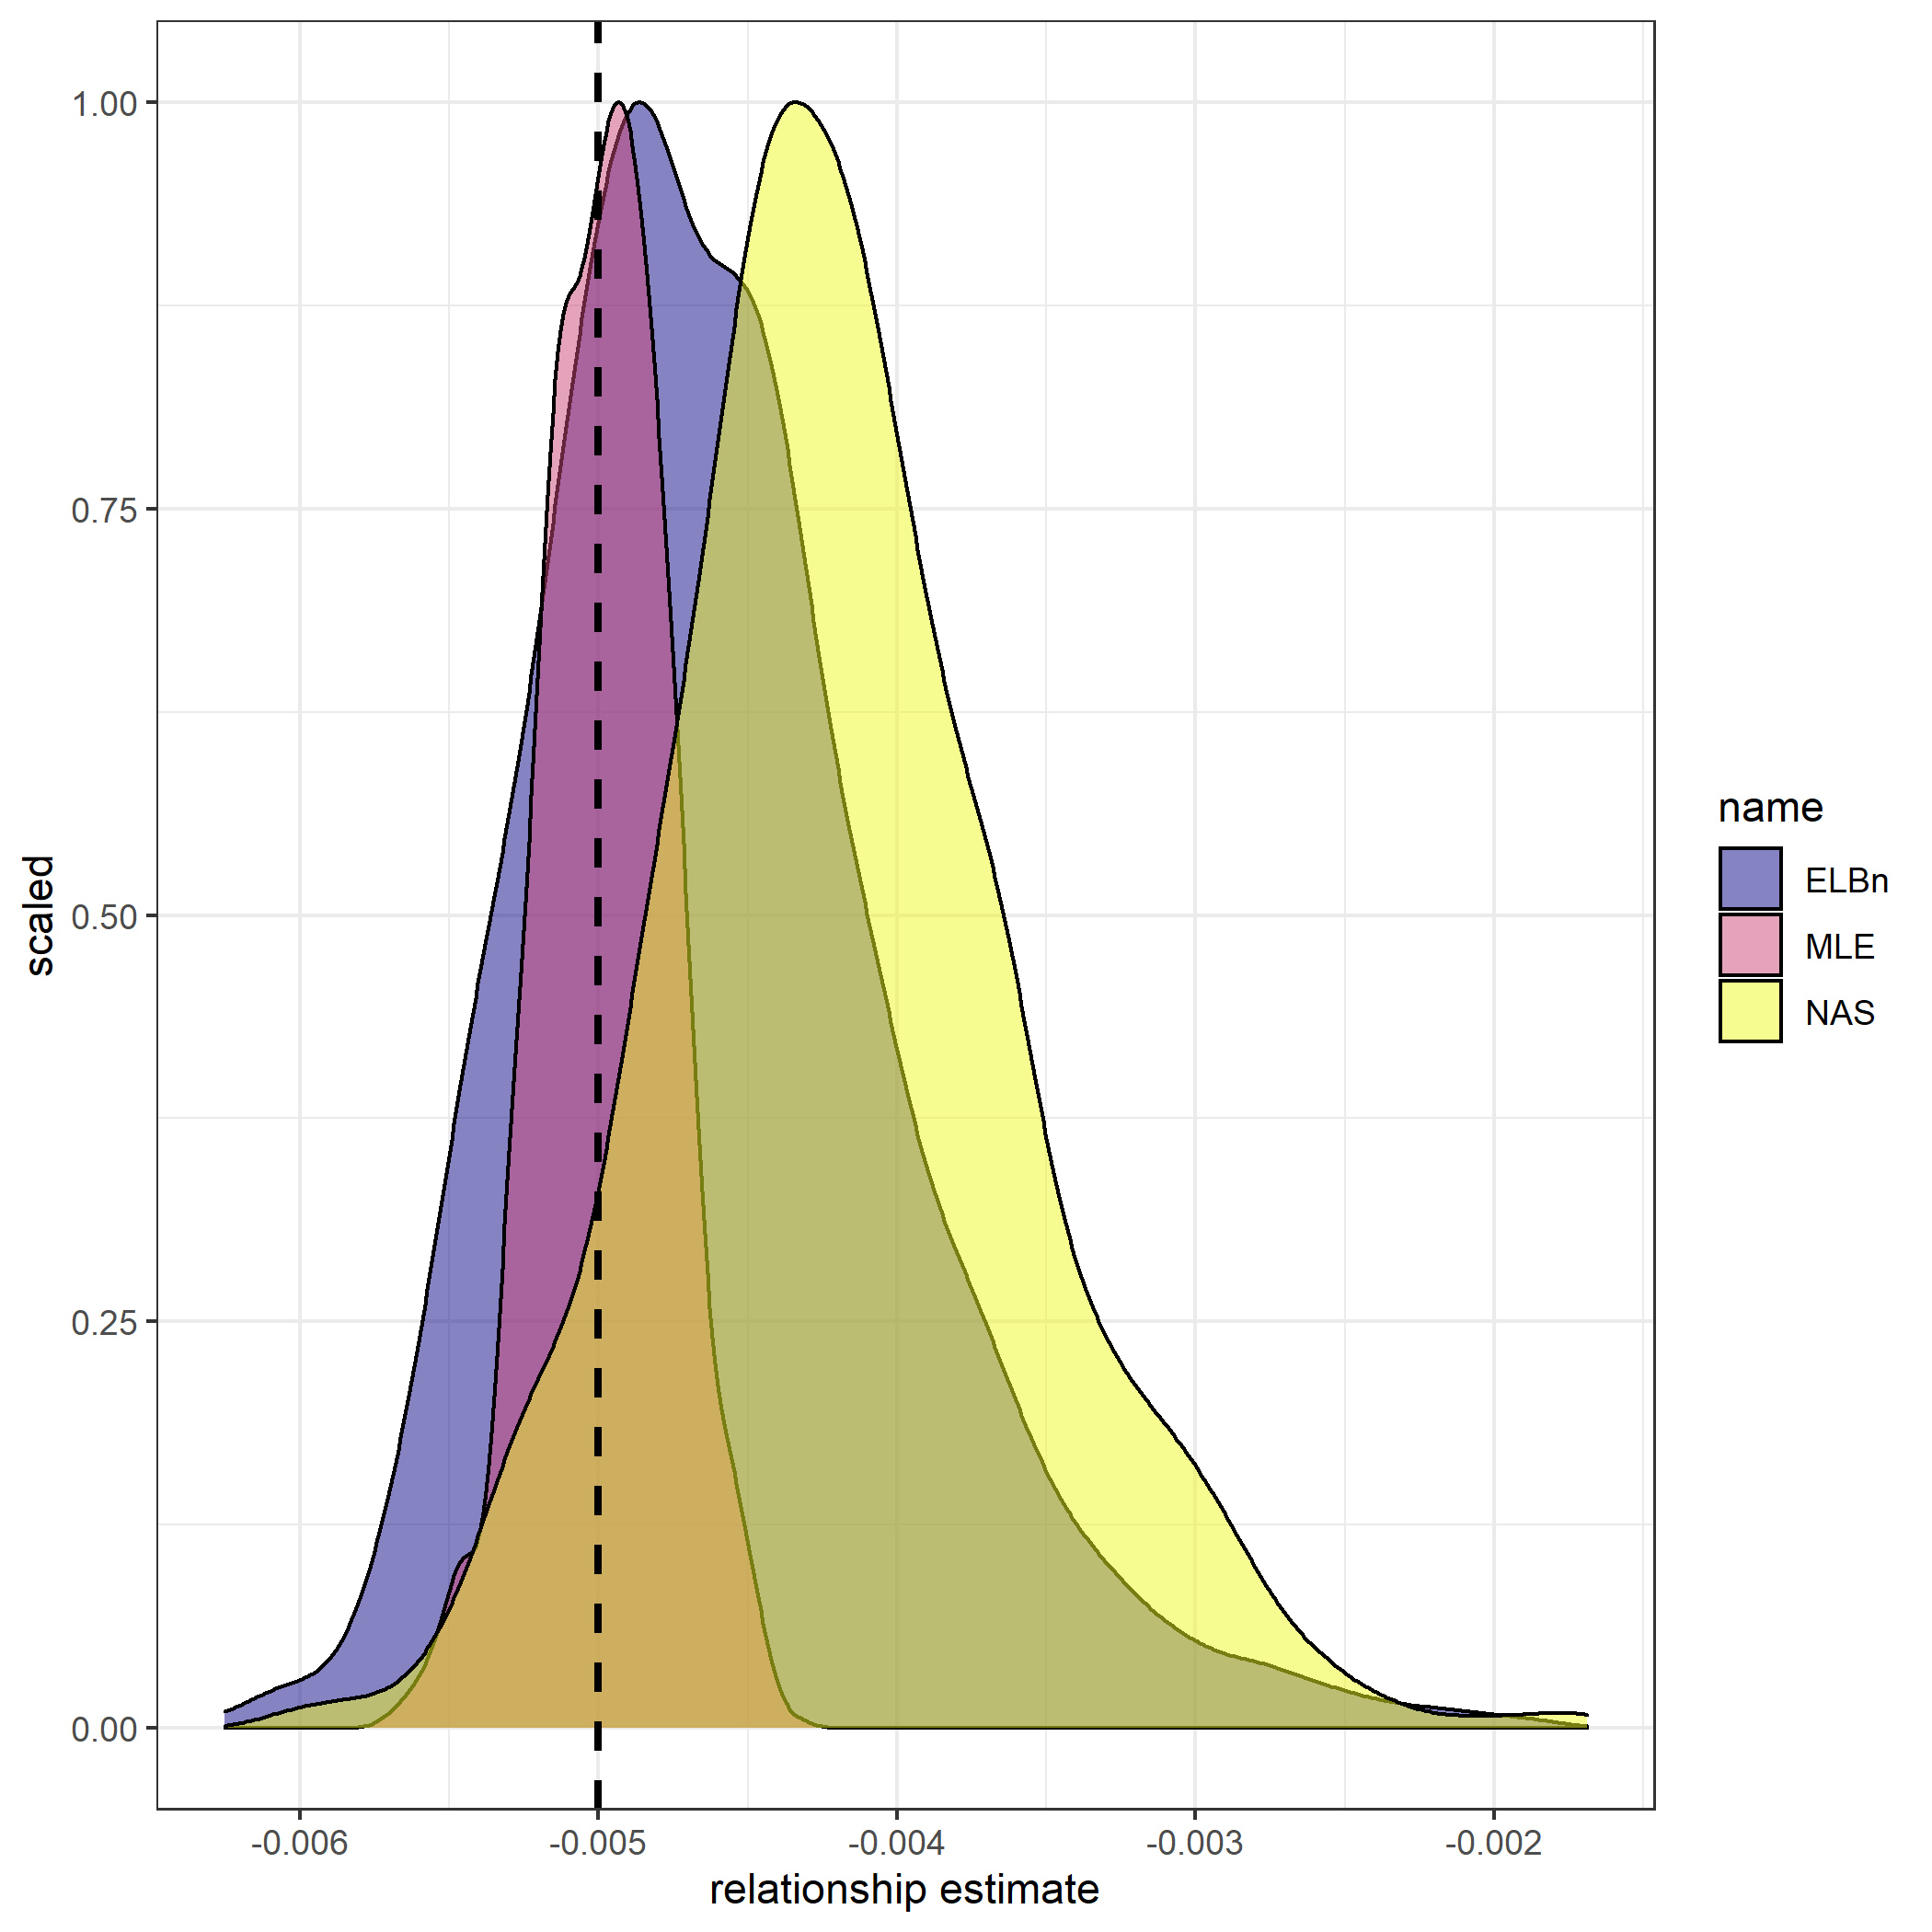
\includegraphics{figures/PLB_large_x_relationship_density.png}
\caption{Relationship estimate}
\end{figure}

\newpage

\hypertarget{range-of-body-sizes-1-to-100}{%
\subsubsection{Range of body sizes = 1 to
100}\label{range-of-body-sizes-1-to-100}}

\begin{figure}
\centering
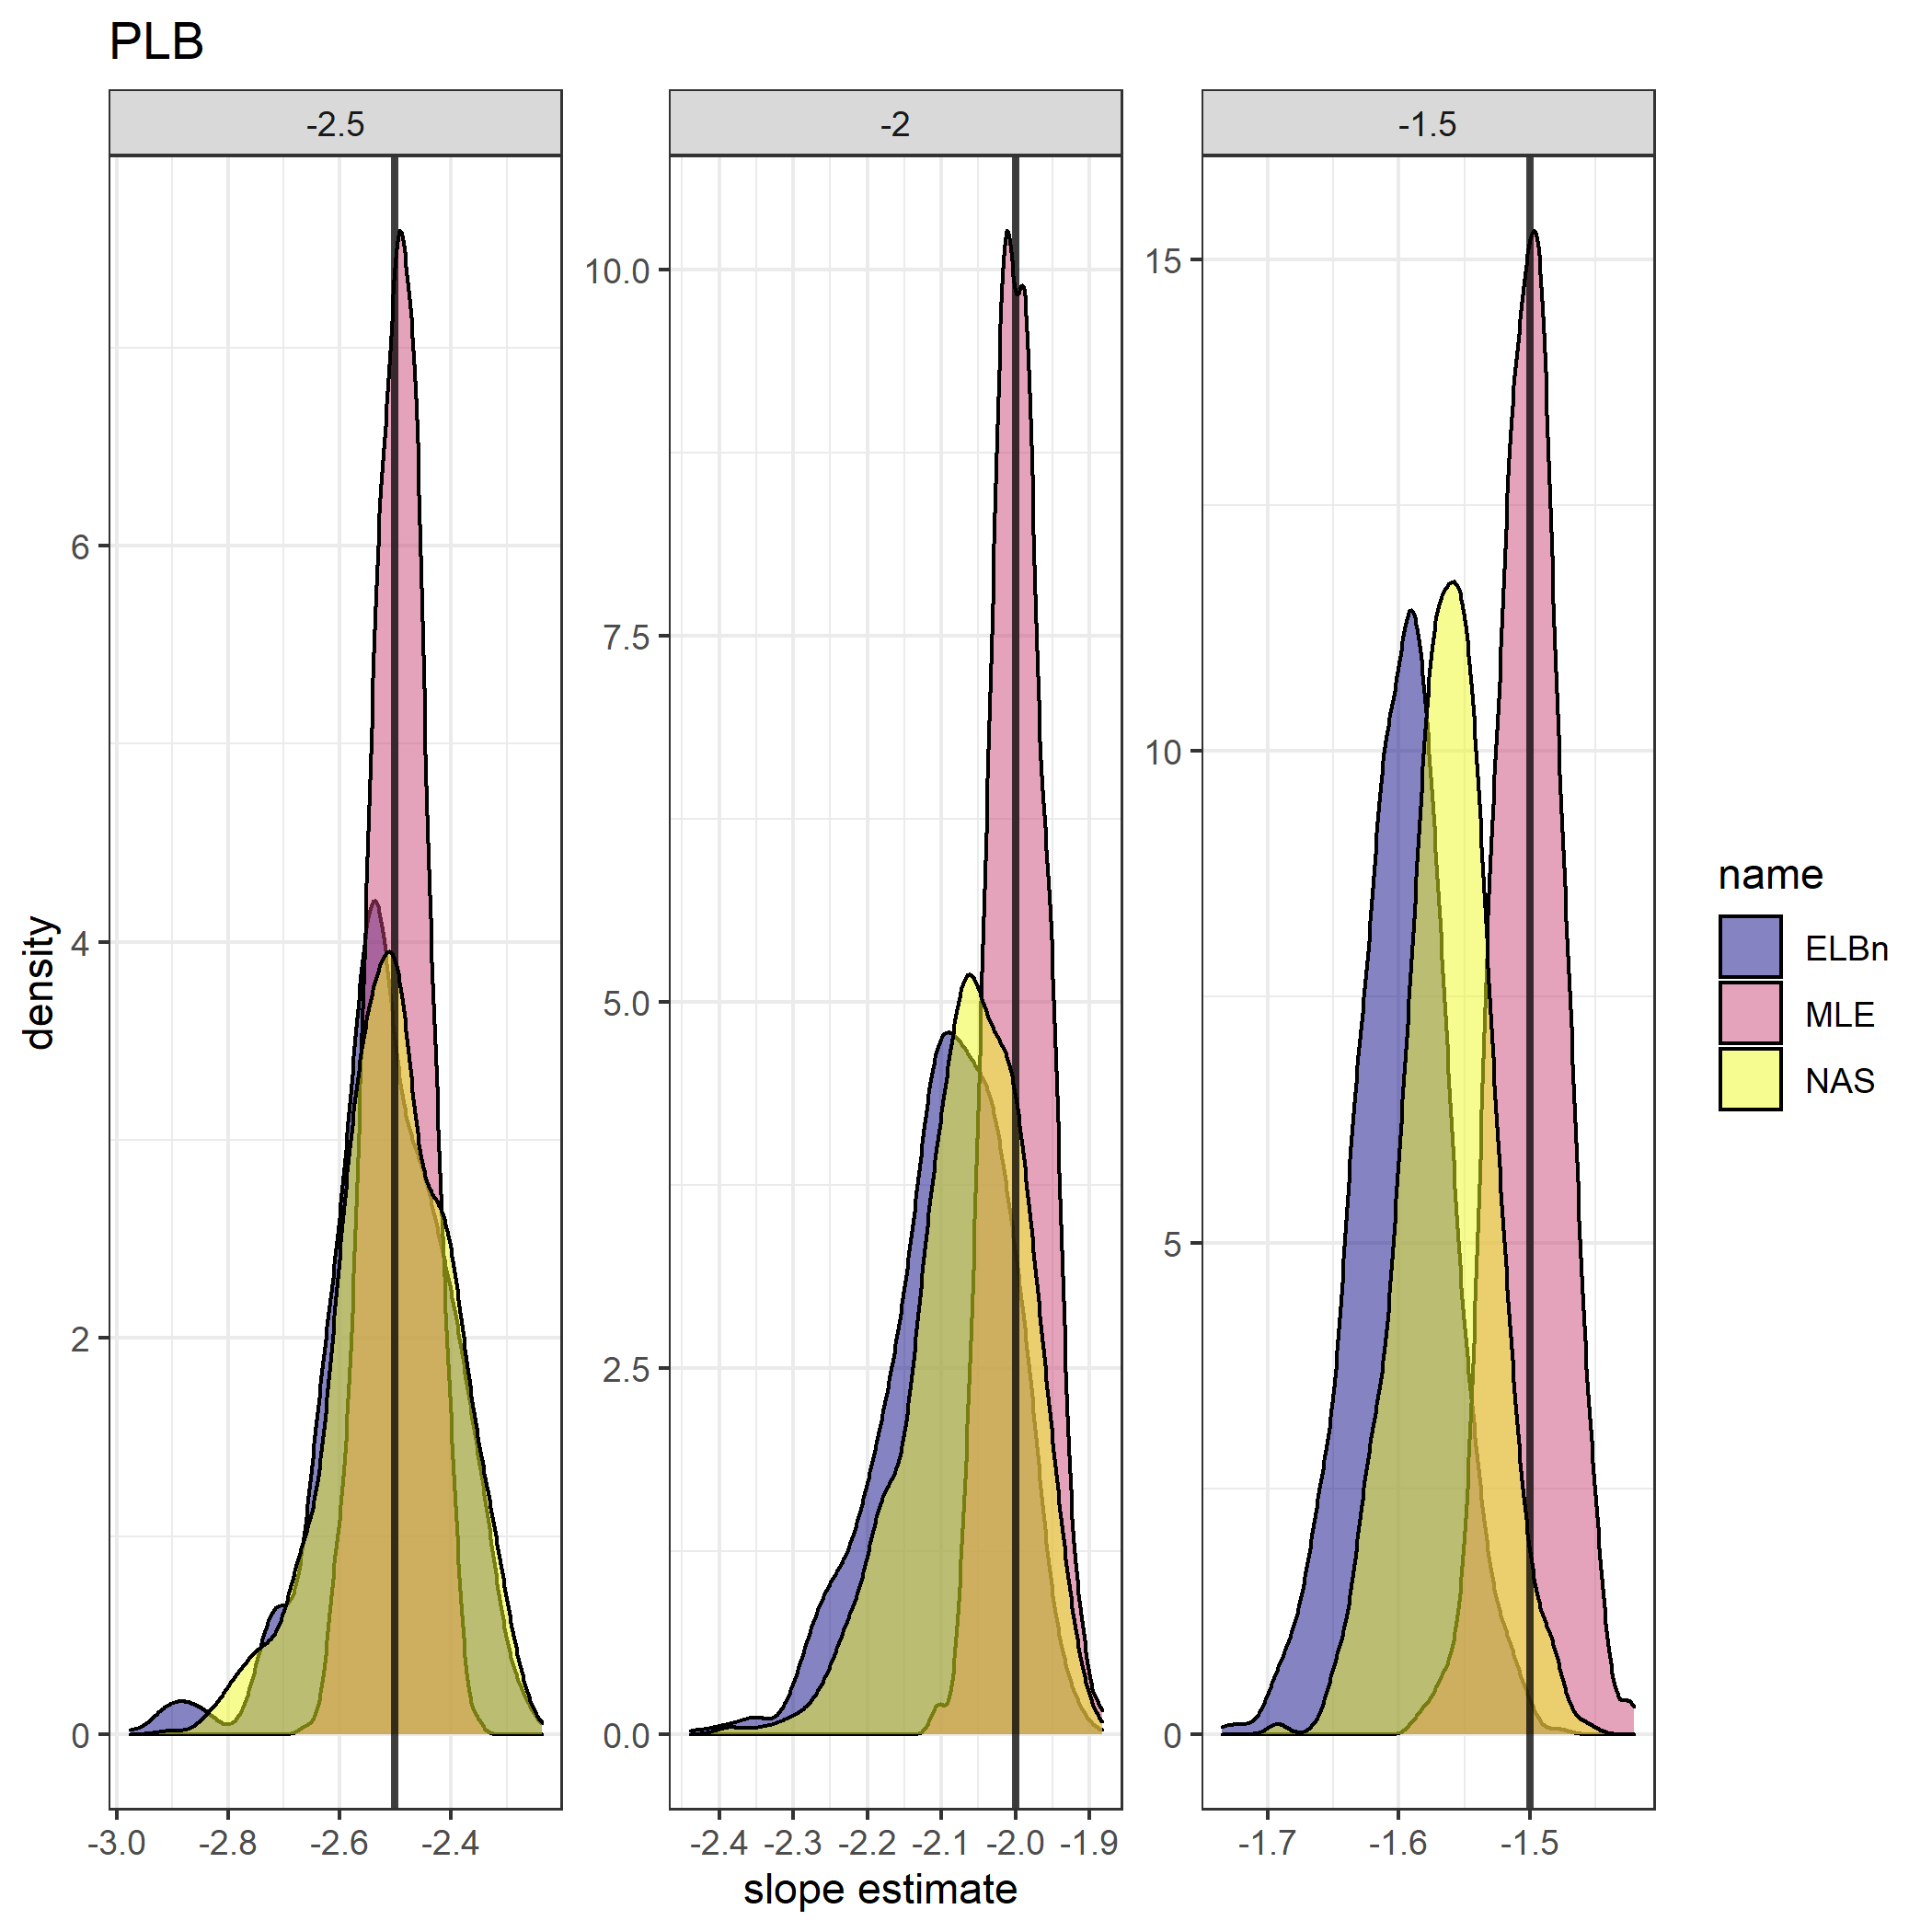
\includegraphics{figures/PLB_small_m_est_b_density.png}
\caption{Distribution of estimated \$\textbackslash lambda\$ coefficient
for five sites across a hypothetical gradient with known values(dashed
line). Range of body sizes is smaller than main anaysis and ranges from
1, to 100.}
\end{figure}

\newpage

\begin{figure}
\centering
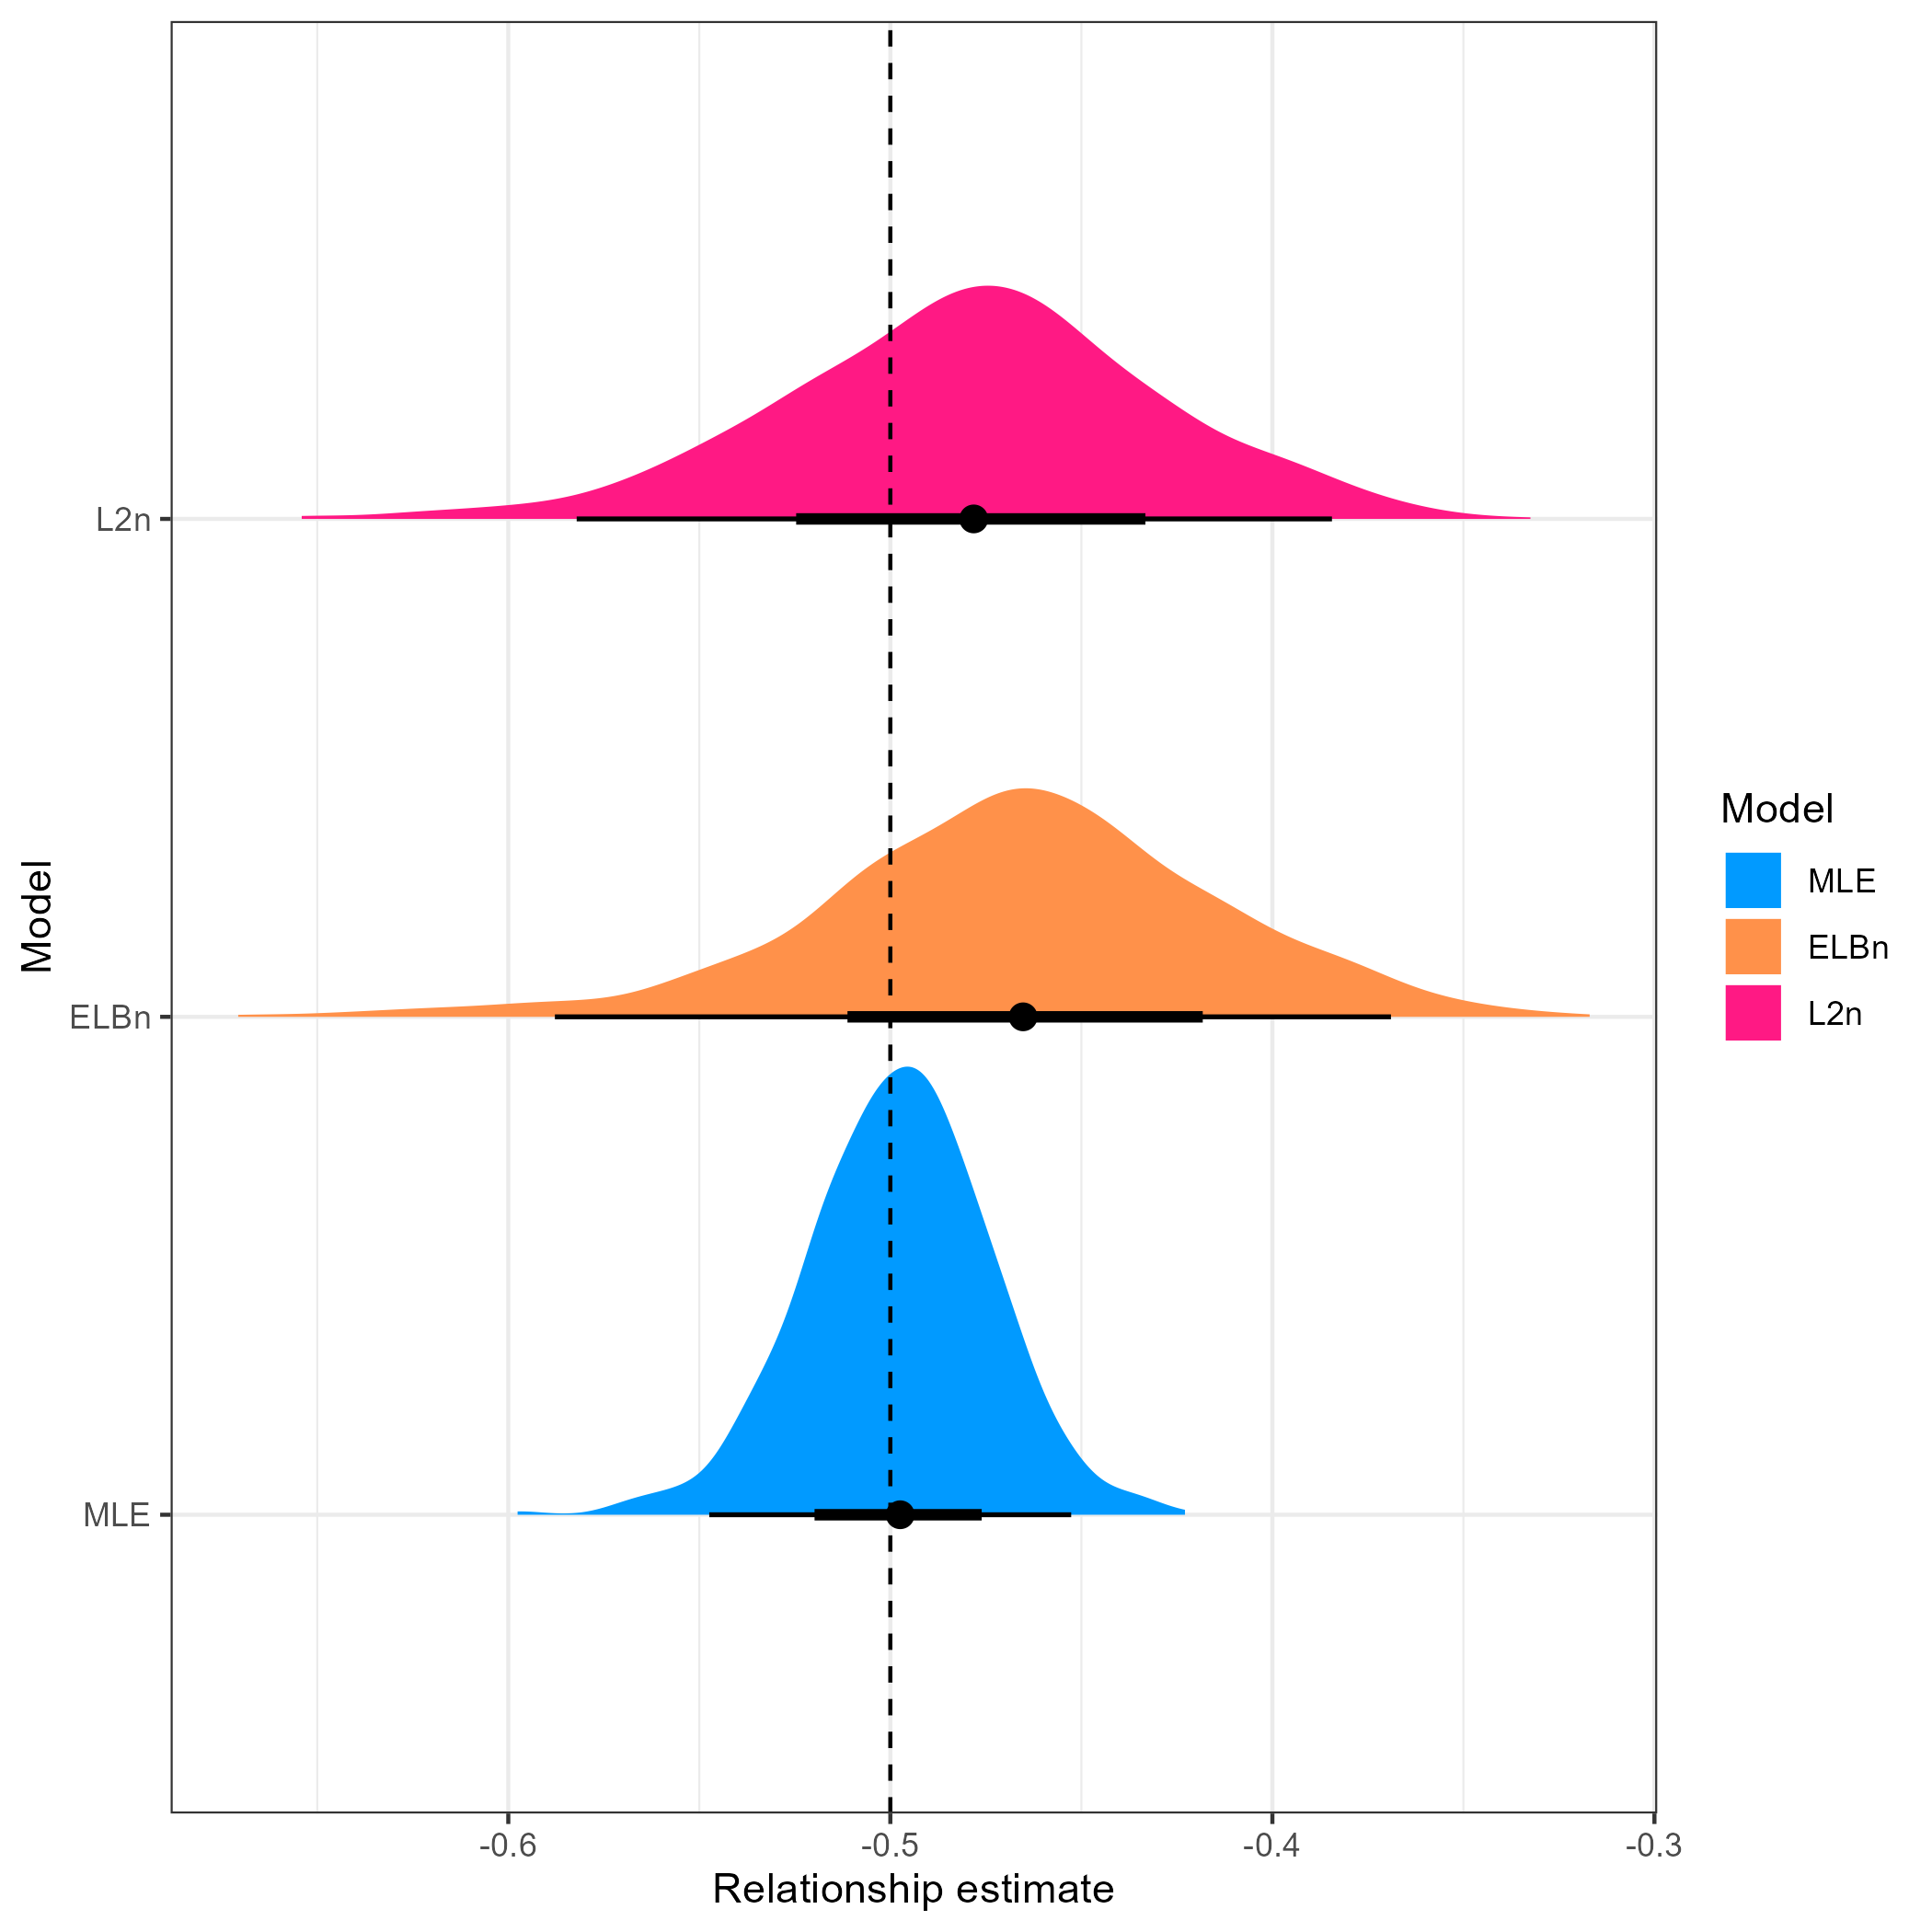
\includegraphics{figures/PLB_small_m_relationship_density.png}
\caption{Relationship estimate}
\end{figure}

\hypertarget{comparison-with-other-published-estimates}{%
\section{Comparison with other published
estimates}\label{comparison-with-other-published-estimates}}

SI Table. This table shows published estimates of the variation in size
spectra slopes (or exponents) in empirical studies. It is unclear how to
directly compare estimates of the slope with different methods.However,
the published estimates here range from \textasciitilde0.1 to 0.2 across
the gradients studied. For comparison, the 2.5-95\% quantiles around the
relationship estimate for the MLE method were \textasciitilde0.1,
whereas for the ELBn and NAS method they were \textasciitilde0.25 and
\textasciitilde0.2, respectively. b\_diff is the change in estimate
(b-low - b-min). System refers to stream communities or mesocosm
experiments. Method: MLE = maximum likelihod estimate, ELB = equal
logarthmic binning, the number before indicates the number of bins used.
The normalization process shifts the estimates by an absolute value of
1.0. Hence, direct comparison the relative change in normalized and
non-normalized studies should not introduce any bias. The O'Gorman et
al.~2017 study used average species size and abundance (Local Size
Density Relationship, \emph{sensu} White et al.~2007) as opposed to
individual size distribution. These methods are related, but it is
unclear how to directly compare estimates from each method.

\begin{Shaded}
\begin{Highlighting}[]
\FunctionTok{read.csv}\NormalTok{(}\StringTok{"lit comparison.csv"}\NormalTok{)}
\end{Highlighting}
\end{Shaded}

\begin{verbatim}
##                                      Author b_diff error error_type b_low
## 1                      Pomeranz et al. 2021   0.12    NA            -1.37
## 2     Yvon Durocher et al. 2011 (Community)   0.13    NA            -0.79
## 3             Dossena et al. 2012 (October)   0.14 0.070         se    NA
## 4                      O'Gorman et al. 2017   0.15    NA            -0.85
## 5                      Martinez et al. 2016   0.15    NA            -1.11
## 6 Yvon Durocher et al. 2011 (Phytoplankton)   0.19    NA            -0.46
## 7                    McGarvey and Kirk 2018   0.19    NA            -1.81
## 8               Dossena et al. 2012 (April)   0.21 0.064         se    NA
##   b_high       System      Driver
## 1  -1.25      Streams Temperature
## 2  -0.92 FW mesocosms Temperature
## 3     NA FW mesocosms Temperature
## 4  -0.70      Streams Temperature
## 5  -0.96      Streams    Land Use
## 6  -0.65 FW mesocosms Temperature
## 7  -1.62      Streams Seasonality
## 8     NA FW mesocosms Temperature
##                                                Method
## 1                                                 MLE
## 2                              10 ELB, not normalized
## 3                               6 ELB, not normalized
## 4 ln (mean species abundance) ~ ln(mean species mass)
## 5                               6 ELB, not normalized
## 6                              10 ELB, not normalized
## 7                                      NAS, Log2 bins
## 8                               6 ELB, not normalized
\end{verbatim}

\end{document}
